% https://github.com/paperswithcode/releasing-research-code
%
% The point of the chapter introduction is to set the scence and explain what you are doing and why.
% Problems that i am tackling here are: Explaining someone might get different results while using the same method with the same configuration this is for the deep learning method.
% If you are going to do a comparison with another method on a different dataset what parameters should you consider changing and apadting and which are less important.
% This is the first time that such a large scale evaluation has been performed in Target Dependent Sentiment analysis and is the first to do it over different domain, type and medium.
%
% The normal question of why did we choose these three different methods:
% 1. Is a deep learning that has been cited many times and reprduced and repeated with different result thus it would be interesting to be able to give a reason why the results are different.
% 2. The linear model allow comparison of more traditional features like the importance of sentiment lexicons and dependency parsers. As we are comparing to models that are the same apart from a dependency parser weather the difference is statitsically signifcant as this was never shown in the original paper.
%
% How can lesson learned from reproducing a method improve evaluative rigour within TDSA? This is relation to random seeds I think that is why I put that here.
% How generalisable are methods within TDSA?
%
%%%%% Need to explain somewhere the reason why it is still important to replicate a method when the code has already been released. I put this as the following within the presentation as COLING: Reproducing methods that have released their code is still a worth while pursuit as reproducing the method from the paper allows us as a community to find out what is missing in our papers that is vital for reproducing our work.

\section[Introduction]{Introduction\footnote{All code that creates the evidence for this chapter can be found in this codebase: \url{https://github.com/apmoore1/thesis-chapter-5-linear-models}. The evidence for table \ref{table:repro_papers_stats} can be found in this codebase: \url{https://github.com/apmoore1/tdsa-paper-details}.}\footnote{A lot of this chapter is based on, extends, and in some places contains complete or paraphrased extracts from \citet{moore-rayson-2018-bringing}.}}
\label{section:repro_intro}

Within this chapter the terms reproduce and replicate will be used frequently. Thus replicate will be defined as ``running the exact same system under the same conditions in order to get the exact same results as output'' \citep{fokkens-etal-2013-offspring}, essentially running the published code from the paper. Reproducing the results requires re-creating a system through different means which should ``lead to the same overall conclusions rather than producing the exact same numbers'' \citep{fokkens-etal-2013-offspring}. 

As highlighted within the literature review (chapter \ref{chapter:lit_review}) there has not been a reproducibility study within the TDSA literature. To many this might not be a problem as most works publish their code alongside the paper as shown by table \ref{table:repro_papers_stats}. However, many of these codebases lack detailed documentation and mainly only provide a script to re-run the experiment, which is perfectly fine, but does mean many of the details of the method are hidden within the codebase. These finer details could well be reported in the paper which overcomes this issue. 

In this chapter, three papers are reproduced: two Neural Pooling (NP) methods\footnote{A Neural Pooling method is a method that aggregates vector values dimension wise. An example use case for NLP is where all \textit{N} words in a text are represented as dense word vectors of dimension size \textit{m}, applying a Neural Pooling method aggregating using the maximum value would return a single word vector of size \textit{m} with the maximum value for each dimension across the \textit{N} words. See \citet{vo2015target} for more information on Neural Pooling.} \citep{vo2015target, wang-etal-2017-tdparse} (which are not based on Neural Networks (NN)), and one LSTM based \citep{tang-etal-2016-effective}. All three have published their code. It is shown for the two NP methods that scaling features, a setting which was not reported in the papers, but for one \citep{wang-etal-2017-tdparse} did mention in part in the documentation of the codebase\footnote{The README which can be found here: \url{https://github.com/bluemonk482/tdparse}.}, can cause significant differences in the results. Further, it is also shown for the NP methods that the C-value within the SVM classifier used in the NP methods can also cause significant differences. This parameter is reported in \citet{vo2015target} but not \citet{wang-etal-2017-tdparse}. Additionally, for the LSTM based method it is shown that reported results are difficult to reproduce without taking into account random seeds, a factor that is never mentioned in the paper and has only recently been shown to be an issue with Neural Network (NN) based methods within NLP \citep{reimers-gurevych-2017-reporting}. The distribution of results generated from different random seeds suggests a possible reason why some prior works, which have attempted to reproduce \citep{tay2018learning} and replicate \citep{chen-etal-2017-recurrent} this LSTM method, reported different results to each other and the original authors. Lastly, a new investigation into using larger more general word embeddings finds that they are at least as good as the original smaller more task-oriented embeddings, resulting in a trade off between performance, efficiency, and convenience. These reproduction findings contribute to answering \rqref{rq:lessons} `what lessons can be learned from reproducing a method within TDSA?'.


\begin{table}[!h]
    \centering
    \begin{tabular}{|p{0.22\textwidth}|p{0.22\textwidth}|p{0.22\textwidth}|p{0.22\textwidth}|}
    \hline
         Number of papers & Code published (\%) &	Code link in paper (\%) &	Code link not in paper (\%)  \\
         \hline
         31 & 16 (51.61\%) & 13 (41.94\%) &	3 (9.68\%) \\
    \hline
    \end{tabular}
    \caption{Out of the 31 papers published between 2013 and 2019 from the relevant NLP conferences (ACL, EACL, NAACL, EMNLP, CONLL, COLING, AAAI, TACL, and IJCAI) and WASSA workshops, this shows how many of them publish their code. Out of those that release their code the number that put a link to their code in the paper compared to those that do not and have to be found through an internet search. Note the author's paper \citep{moore-rayson-2018-bringing} is not included in the statistics.}
    \label{table:repro_papers_stats}
\end{table}

The second half of the chapter explores \rqref{rq:generalisable} `how generalisable are existing methods within TDSA?'. This research question was motivated in part by the fact that many methods do not make use of the datasets that exist\footnote{Or existed at the time.} as shown by table \ref{table:repro_methods_datasets_used}. Additionally these existing datasets often vary by type (e.g. review, social media, or news), domain (e.g. products), medium (e.g. written or spoken), dataset size, language, and many other factors. Thus, evaluating a method only on a subset of existing datasets limits the conclusions that can be drawn from those evaluated methods as they might perform well on those evaluated datasets, but it is unknown if they perform well on datasets from a different medium, domain, etc. Therefore to answer the research question, the reproduced TDSA methods from the first half of the chapter, which were selected due to their methodological differences, are applied to six English TDSA datasets. These six datasets vary by the following classes: domain, type, and medium as shown by table \ref{table:repro_dataset_stats} (see the experimental setup section \ref{section:repro_experimental_setup} for more details on the datasets used). This is the first large scale TDSA experiment that has evaluated a range of methods across all three classes. Doing so allows the methods to be tested for generalisation as none of them were originally developed for all six datasets. This research finds that methods are more affected by dataset size and sentiment class distributions than type, domain, and medium. Further, when controlling the dataset size the LSTM methods are greatly affected in comparison to the NP methods. These findings have important consequences as they bring to light to some extent when to use which method.  


%methods that were state of the art at the time on the selected dataset(s) is not the case on all. Additionally it shows that no one method is best on all datasets, showing that no method is state of the art, but rather state of the art on a particular subset of datasets. Lastly it is found that methods from the same paper do not keep their performance ranking when trained and tested on new unseen datasets. These findings have important consequences as they bring to light to some extent when to use which method.  

%This therefore requires several different TDSA methods thus we use those that have been reproduced, two NP and one LSTM, as all three are different. Furthermore the methods are evaluated on seven different TDSA dataset that vary by domain (e.g. product), type (e.g. review, social media), and medium (e.g. written, speech). This is the first TDSA evaluation that has been performed where methods have been evaluated across three different dataset classes (domain, type, and medium). In doing so allowing the methods to be tested for generalisation as none of them were originally developed for all seven datasets. This study finds that methods that were SOTA at the time on one dataset is not the case on all. Additionally it shows that no one method is best on all datasets, showing that no method is state of the art but rather state of the art on a particular subset of datasets. Lastly it is found that methods from the same paper do not keep their performance ranking when trained and tested on new unseen datasets. 

\begin{table}[!h]
    \centering
    \begin{tabular}{|p{6cm}|k|g|k|y|d|d|d|}
\hline
 &  \multicolumn{7}{c|}{Datasets}  \\
\hline
Methods & \textbf{1} & 2 & \textbf{3} & \textbf{4} & \cellcolor{green}{5} & \cellcolor{pink}{\textbf{6}} & \cellcolor{pink}{\textbf{7}}\\
 \hline
 \citet{mitchell-etal-2013-open} & \cellcolor{gray} &  & \cmark   & \cellcolor{gray} & & &\\
 \hline
 \citet{kiritchenko-etal-2014-nrc} & \cellcolor{gray} &  &  & \cmark &  &  &\\
 \hline
 \citet{dong-etal-2014-adaptive} & \cmark &  & & \cellcolor{gray} & & &\\
 \hline
 \textbf{\citet{vo2015target}} & \cmark &  &   & & & & \\
 \hline
 \citet{zhang-etal-2015-neural} & &  & \cmark  & & & &\\
 \hline
 \citet{zhang2016gated} & \cmark & \cmark & \cmark  & & & & \\
 \hline
 \textbf{\citet{tang-etal-2016-effective}} & \cmark &   &  &  & & &\\
 \hline
 \citet{tang-etal-2016-aspect}& & &   & \cmark & & &\\
 \hline
 \citet{wang-etal-2016-attention} & &  & & \cmark & & &\\
 \hline
 \citet{chen-etal-2017-recurrent} & \cmark &  &   & \cmark & \cellcolor{green}{\cmark} & &\\
 \hline
 \citet{liu-zhang-2017-attention} & \cmark & \cmark & \cmark  &  & &  & \\
 \hline
 \textbf{\citet{wang-etal-2017-tdparse}} & \cmark & &   &  &  & \cellcolor{pink}{\cmark} &\\
 \hline
 \citet{marrese-taylor-etal-2017-mining} & &  & &   \cmark & &  & \cellcolor{pink}{\cmark}\\
 \hline
\multicolumn{8}{|p{11.5cm}|}{\textbf{1}=\citet{dong-etal-2014-adaptive}, 2=\citet{wilson2008fine}, \textbf{3}=\citet{mitchell-etal-2013-open}, \textbf{4}=\citet{pontiki-etal-2014-semeval}, 5=\citet{chen-etal-2017-recurrent}, \textbf{6}=\citet{wang-etal-2017-tdparse}, \textbf{7}=\citet{marrese-taylor-etal-2017-mining}}\\
\hline
\multicolumn{8}{|p{11.5cm}|}{\centering \cbox{pink} Social Media \quad \cbox{yellow} Reviews \quad \cbox{green} News \quad \cbox{gray} Not Applicable}\\
\hline
\end{tabular}
    \caption{A tick denotes that the method in the row has been applied to the dataset in the column, from the method's original paper and not a replication/reproduction of the method. Methods in \textbf{bold} are those that are being reproduced in this chapter. The dataset numbers in \textbf{bold} are the datasets that the reproduced methods will be evaluated on in this chapter. The colours represent the type of the dataset, apart from not applicable which indicates the dataset did not exist when the method was created.}
    \label{table:repro_methods_datasets_used}
\end{table}

%The evaluation of different methods has become more problematic over the years as more ever increasingly complex methods have come about. Therefore the importance of comparative evaluation becomes ever more important. Comparative evaluation can become more challenging when the evaluation is across multiple datasets with different properties for example different domain (politics, electronics), medium (spoken text, written), and type (social media, review). Each one these properties may cause adjustments in the methods to get a fair comparison, for example a method that uses a dependency parser may perform significantly better when the parser being used has been created for the data that it is being applied too rather than a different data type\slash domain\slash medium. Therefore knowing what changes to a method that are significant to its performance given the dataset properties is important for fair comparison. This is crucial with respect to comparing previous state of the art results that have a different evaluation setup e.g. use a different word embedding, dependency parser, tokeniser etc. Thus one major contribution of this section is quantifying the importance of evaluation setup, by evaluating methods across numerous different parameters/settings of the methods across different datasets that contain different properties. This is of great importance as some methods have used domain specific settings e.g. word embeddings \citep{vo2015target,zhang2016gated,wang-etal-2017-tdparse} and are therefore not comparable to methods that do not \citep{chen-etal-2017-recurrent,li-etal-2018-transformation} unless they are re-run or reproduced. Therefore quantifying the difference in methods between these domain specific settings could allow comparability without the need for re-running or reproducing.
%Furthermore knowing which parameters/settings affects the methods can help guide future researchers and practitioners choose sensible default parameters/settings before adapting the methods to their own needs.
%\todo[inline]{A potential research questions is What properties within a method are significantly important to the performance of the method and how they relate to different dataset properties?}
%\\


% This paper: Target-Sensitive Memory Networks for Aspect Sentiment Classification
% Must have reproduced the work from Wang et al 2016 which is the ATAE method as they show macro F1 scores but the original only looked at accuracy.
%Another equally important and related problem is that of reproducability. Some work within Target Dependent Sentiment Analysis (TDSA) reproduce or re-use the code of previous works to circumnavigate\comment{is avoid a better word?} the evaluation setup problem stated above \citep{chen-etal-2017-recurrent,tay2018learning}. However this can be shown to be difficult through a couple of works \citep{chen-etal-2017-recurrent,tay2018learning} that could not re-run or replicate respectively successfully one particular deep learning method \citet{tang-etal-2016-effective} when using the same datasets and evaluation setup. In this chapter we show a potential reason why this maybe the case, as well as highlighting other important parameters/settings that are missing from the original papers that are critical to replicating the three chosen methods. This chapter also shows the (obvious?) relation between significantly important parameters/settings and the parameters that are stated within the paper to allow others to successfully replicate the method.\\
%\\

% Need to add into this paragraph something to do with generalisability I think with regards to the evaluation across numerous datasets and the results from that.


%The chapter concludes with a mass evaluation across multiple datasets on the methods that have been replicated within the chapter using the optimal parameters found for each method on each dataset. This mass evaluation will be a first within TDSA as the English datasets will come from three different dataset properties; 1. domain, 2. type, and 3. medium. From this the community can have a strong baseline of methods to compare to across all of these datasets. This will also be the first time the community will know the true general State Of The Art (SOTA) within TDSA as previous results only state their results for a limited number of datasets and therefore are not general enough to compare to.\\
%\\
%In summary this chapter demonstrates the importance of parameters within TDSA methods and how these relate to the replicability of the method from the paper. Lastly it highlights the under utilisation of English datasets within TDSA and the importance of them with regards to generalisability of methods within TDSA. The chapter is structured as follows; first explain the three different methods that are being replicated. The second section shows how they were successfully replicated. The third section reveals the importance of different parameters within a method and the importance of these parameters in replicating the original work. The last section presents the mass evaluation results.

\section{Related Work}
Reproducibility and replicability have long been key elements of the scientific method, but have been gaining renewed prominence recently across a number of disciplines with attention being given to a `reproducibility crisis'. For example, in pharmaceutical research, as little as 20-25\% of papers were found to be replicable \citep{prinz2011believe}. The problem has also been recognised in computer science in general \citep{collberg2016repeatability}. Reproducibility and replicability have been researched for sometime in  Information Retrieval (IR) since the Grid@CLEF pilot track \citep{ferro2009clef}. The aim was to create a `grid of points' where a point defined the performance of a particular IR system using certain pre-processing techniques on a defined dataset.
\citet{louridas2012note} looked at reproducibility in Software Engineering after trying to replicate another author's results and concluded with a list of requirements for papers to be reproducible: (a) All data related to the paper, (b) All code required to reproduce the paper, and (c) Documentation for the code and data. \citet{fokkens-etal-2013-offspring} looked at reproducibility in WordNet similarity and Named Entity Recognition, finding five key aspects that cause experimental variation and therefore need to be clearly stated: (a) pre-processing, (b) experimental setup, (c) versioning, (d) system output, and (e) system variation. In Twitter sentiment analysis, \citet{sygkounas2016replication} stated the need for using the same software library versions and datasets when replicating work.

Different methods of releasing datasets and code have been suggested. \citet{ferro2009clef} defined a framework (CIRCO) that enforces a pre-processing pipeline where data can be extracted at each stage therefore facilitating a validation step. They stated a mechanism for storing results, dataset and pre-processed data\footnote{\url{http://direct.dei.unipd.it/}}. \citet{louridas2012note} suggested the use of a virtual machine alongside papers to bundle the data and code together, while most state the advantages of releasing source code \citep{fokkens-etal-2013-offspring, potthast2016wrote, sygkounas2016replication}. 

Within the the research community, conferences have added reproducible research as a research track, and this started within IR in 2015\footnote{\url{http://ecir2015.ifs.tuwien.ac.at/wp/?page_id=227}}. These tracks have now progressed into NLP with COLING 2018\footnote{\url{https://coling2018.org/index.html\%3Fp=491.html}}, LREC 2018\footnote{\url{http://lrec2018.lrec-conf.org/en/calls-papers/1st-call-papers/}}, LREC 2020\footnote{\url{https://lrec2020.lrec-conf.org/en/calls-papers/1st-call-papers/}}, and COLING 2020\footnote{\url{https://coling2020.org/pages/call_for_papers}}. Furthermore, LREC 2020 also had the first shared task on reproducing a set of NLP papers \citep{branco-etal-2020-shared}. Predating these reproducible research tracks at NLP conferences was the 4REAL workshop\footnote{\url{http://4real.di.fc.ul.pt/}} which encouraged researchers to present and generate reproducible NLP research.


More recently within the NLP and ML fields there has been a growing consensus around what is required to make a paper reproducbilble, with the EMNLP 2020 conference using a checklist derived from \citet{dodge-etal-2019-show} and the NeurIPS 2020 conference checklist by Joelle Pineau\footnote{\url{https://www.cs.mcgill.ca/~jpineau/ReproducibilityChecklist.pdf}}. There has also been a push for better reporting of methods, which relates to the concept of generalisation as well as reproducibility within this thesis. A model card \citep{mitchell2019model} is one form of reporting a method whereby the creator(s) of the method would state various details of the method including ethical information, method details, and evaluative results. Companies have also created tools to make machine learning more reproducible such as Weights \& Biases\footnote{\url{https://www.wandb.com/}} `Artifacts'\footnote{\url{https://www.wandb.com/articles/announcing-artifacts}} that allows users to track the data and code that created a specific model.







%More recently within reproducibility \citet{yang-etal-2018-design} methodically explored different configurations of a neural sequence labelling system, these configuration changes included different layers the network, optimiser, tagging scheme, embeddings, and runtime environment.   

% Maybe put something here on the data, model cards etc. Then after that mention the dodge work. Within the paragraph after that mention the work within NER and Mass eval at COLING 2018 or this might be better above.

More closely related to TDSA, \citet{marrese-taylor-matsuo-2017-replication} attempted to reproduce three different syntactic target extraction methods. They found that parameter tuning was very important, however using different pre-processing pipelines such as Stanford's CoreNLP did not have a consistent effect on the results. They found that the methods stated in the original papers are not detailed enough to reproduce the study as evidenced by their large results differential. Within sentiment classification at the document level \citet{dashtipour2016multilingual} reproduced numerous non Neural Network (NN) multilingual methods and applied them all to the same two datasets so that the methods can be easily compared. At the sentence level \citet{barnes-etal-2017-assessing} compares seven NN and non-NN approaches on six datasets, where many of these datasets have only been benchmarked against one approach. They found a bi-directional LSTM to be on average the most effective approach, and further found that using pre-trained sentiment embeddings from lexically similar data as the training data greatly improves results. Lastly within TDSA, \citet{chen-etal-2017-recurrent} reproduced multiple methods and created their own methods, which they then applied to four datasets, which contain two different languages, different domains, and types, but all come from the same medium, written text. Thus, this chapter presents the first reproduction study within TDSA. Also using the methods reproduced that are known to reflect the original paper's implementation, the largest to date study of generalisation within TDSA within the English language that spans six datasets with different types, domains, and mediums.

\section{Methods}
\label{section:repro_methods}
% In this section I need to introduce the three methods that I am going to replicate, the reason these were chosen other than they are popular within the literature. Then go throught each method explaining the method and showing a diagram of the method.

In this chapter, three popular TDSA methods are reproduced, two NP; \citet{vo2015target} and \citet{wang-etal-2017-tdparse}, and one LSTM \citet{tang-etal-2016-effective}. The LSTM based method was chosen due to the disagreement within the literature, where different prior works have reported different results to the original. The other two methods were chosen as they are fairly different to the LSTM whereby they use word embeddings, but those word embeddings are only input into an SVM compared to a large parameterised LSTM. Secondly within the two NP methods \citet{wang-etal-2017-tdparse} is a direct extension of \citet{vo2015target} whereby they include syntactic information directly into the model thus requiring a dependency parser. Therefore all three methods are fairly different. These differences are important in evaluating how generalisable the methods are across varying datasets as stated in the introduction \ref{section:repro_intro}, as these differences could explain why one method is better than another on certain datasets. Furthermore, even though all three have been compared within \citet{wang-etal-2017-tdparse}, they have only been compared on Twitter based datasets and not a range of non-Twitter datasets. In this subsection the three methods will be explained in detail, in the following order: \citet{vo2015target} NP method, \citet{wang-etal-2017-tdparse} NP with dependency parsing, and \citet{tang-etal-2016-effective} LSTM. 


%of which the first two use linear Support Vector Machines (SVM) while the last is a non-linear Long Short Term Memory (LSTM) Neural Network (NN) model. These three methods were chosen due to the difference in approach; NN compared to SVM, the use of 

%We first explain each method we replicated, and show how we have successfully replicated the methods on the datasets they were originally evaluated on. We then 

%We then expand the evaluation setup to include more datasets to increase the coverage and generalisability of the results from these methods. Using this expanded evaluation setup we explore the importance of different parts of these methods and outline which are the most volatile to change with respect to the results. Furthermore due to the increase in the expanded datasets we can find out whether different parameter are more sensitive to different domains, mediums, and/or types.  

\subsection{Neural Pooling}
%  They take the word vectors of the left and right side of the target word, as well as the target word and full text.
The \citet{vo2015target} NP method is the simplest of the three methods being presented within the chapter. As shown in figure \ref{fig:repro_np_architecture} it treats each word in the sentence as a word vector that has come from a pre-trained word embedding model, e.g. GloVe \citep{pennington-etal-2014-glove}. From this the method splits the sentence into four different contexts based on the target word(s) position:

\begin{enumerate}
    \item The whole context -- the whole sentence.
    \item The left context -- all words left of the target word but not including the target word.
    \item The target context -- the target word(s) (can be more than word e.g. camera lens).
    \item The right context -- all words right of the target word but not including the target word.
\end{enumerate}

From these variable length contexts, numerous NP methods are applied to these contexts, to create fixed length feature vectors from a variable length sentence. An NP method as stated takes a variable number of word vectors e.g. $W \in \mathbb{R}^{d\times n}$ where $n$ is the number of words and $d$ is the dimension of the word vector which represent features of the word. The NP then applies a pooling method e.g. maximum value across all the $d$ dimensions of the $n$ words to output a feature vector of $w \in \mathbb{R}^{d}$ in the example. For each context and NP method a feature vector is created, all feature vectors are then concatenated and are inputted into the linear SVM to classify the sentiment of the target.

The method described above is the general approach \citet{vo2015target} took. More specifically they created four different methods which all used the same NP method but different contexts and one also incorporated sentiment lexicons in a novel way, these are described below:

\begin{enumerate}
    \item Target-Independent (TI) -- Only used the whole context.
    \item Target-Dependent Minus (TDM) -- Left, right, and target contexts.
    \item Target-Dependent (TD) -- Left, right, target, and whole contexts (Union of the first two methods).
    \item Target-Dependent Plus (TDP) -- This incorporated sentiment lexicons by filtering all words that are not in the sentiment lexicon from a given context. This sentiment filtering was applied to the left and right contexts denoted as \textit{LS} and \textit{RS} respectively. In total this method used the left, right, target, whole, \textit{LS}, and \textit{RS} contexts.
\end{enumerate}

As can be seen above each method from the top of the list incorporates more context or external information as you move down the list of methods. Furthermore from the methods above only the first method will always produce the same sentiment no matter the target word if all targets come from the same sentence, as it does not incorporate any target information.

This method had several important contributions; first is the splitting up of the sentences into different contexts to model simple interaction between the different contexts. Second the use of sentiment lexicons to filter words when the words are represented as word vectors within sentiment analysis. Lastly the extension of NP methods from \citet{tang-etal-2014-learning} original \textit{max}, \textit{min}, and \textit{avg} functions to those listed below with the contribution of also explaining what the functions capture with regards to sentiment:
\begin{enumerate}
    \item \textit{max} - Maximum value represents positive sentiment.
    \item \textit{min} - Minimum value represents negative sentiment.
    \item \textit{avg} - Average value represents the average sentiment.
    \item \textit{std} - Standard deviation represents the sentiment variation.
    \item \textit{pro} - Product represents the average sentiment but with larger differences between positive and negative sentiment.
\end{enumerate}
Overall the general architecture of \citet{vo2015target} can then be summarised through figure \ref{fig:repro_np_architecture}. 

%This is the first and most simple of the Neural Pooling (NP) methods that has been applied to TDSA. They create different contexts from the text and for each of these contexts they perform maximum, minimum, average, standard deviation, and product pooling over the word embeddings. These pooling features are then inputted into a Support Vector Machine (SVM) to classify the text.

%They created four main contexts that made up four different methods they tested to show the importance of these different contexts. The four main methods and their contexts are explained below:
%\begin{enumerate}
%    \item \textbf{Target-Ind} -- Only the full text contexts.
%    \item \textbf{Target-Dep}- -- Left and right context of the target word and the target word context.
%    \item \textbf{Target-Dep} -- The full text contexts as well as the contexts of \textbf{Target-Dep-}
%    \item \textbf{Target-Dep+} -- All the contexts of \textbf{Target-Dep} as well as additional left and right context where the embeddings are only of the words that appear in the given sentiment lexicon (LS and RS contexts).
%\end{enumerate}
%As might be obvious each method tends to improve upon the other be including more contexts. Furthermore the \textbf{Target-Ind} method is the only method above that will not produce a different sentiment score if two targets are in the same sentence, as it only contains sentence level features and no target specific features. These different contexts are also explained through figure \ref{fig:repro_vo_method}.
\begin{figure}[!h]
    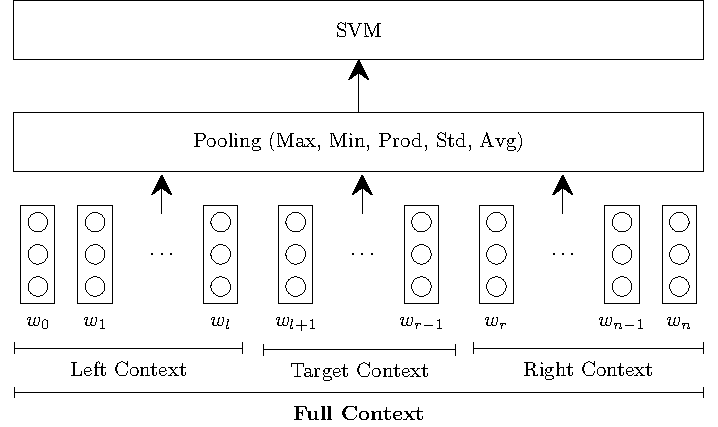
\includegraphics{Diagrams/Reproducibility/vo_method.pdf}
    \caption{General architecture of \citet{vo2015target} and \citet{wang-etal-2017-tdparse}.}
    \label{fig:repro_np_architecture}
\end{figure}
\newpage


\subsection{Neural Pooling with Dependency Parsing}
The \citet{wang-etal-2017-tdparse} method is a direct extension of \citet{vo2015target} where they keep the same NP methods and general architecture but change the contexts. The main motivation of \citet{wang-etal-2017-tdparse} is to improve the simple interaction of the different contexts by incorporating the syntactic structure of the target word using a dependency parser. In more detail this dependency context contains the target word and all connected words within the same root. This makes the assumption that the dependency parser that is used can create multiple roots from one text as it assumes the text is made of more than one sentence. If the dependency parser does not create more than one root in a text then the dependency context will be the same as the whole context\footnote{More precisely it will be the same as the whole context with the target word(s) removed, so very similar to the whole context. A python notebook demonstrating the fact that the authors used the dependency parser (TweeboParser) like this and if another parser is used e.g. Stanford the dependency context will be similar to the whole context can be found here: \url{https://github.com/apmoore1/Bella/blob/master/notebooks/tdparse\_parser.ipynb}.} from \citet{vo2015target} method. The dependency parser they therefore used was the TweeboParser \citep{kong-etal-2014-dependency}\footnote{To the author's knowledge it is believed TweeboParser is the only dependency parser that creates multiple roots for a given text. However the author is not an expert within the field of dependency parsing.} which was created for noisy text such as Tweets and hence why multiple roots can occur in one text. This parser was also used because it was especially created for noisy text and the datasets that \citet{wang-etal-2017-tdparse} applied this method to were Twitter datasets. Thus one expects that this method will work best on social media type of texts as this method has been developed with this bias.

As with \citet{vo2015target}, \citet{wang-etal-2017-tdparse} had three different models each containing either more contexts or external information, these are described in more detail below:

\begin{enumerate}
    \item TDParse Minus -- Only used the dependency context.
    \item TDParse -- Left, right, target, and dependency contexts.
    \item TDParse Plus -- Left, right, target, dependency, \textit{LS}, and \textit{RS} contexts.
\end{enumerate}

Overall the general architecture of \citet{wang-etal-2017-tdparse} is in essence the same as that of \citet{vo2015target}, thus can then be summarised through figure \ref{fig:repro_np_architecture}. 

\subsection{LSTM}
\label{section:repro_lstm_description}

Unlike the previous two methods this is a NN method, and it was the first for TDSA to use an LSTM. \citet{tang-etal-2016-effective} created three different methods: 

\begin{enumerate}
    \item Standard LSTM (LSTM).
    \item Target Dependent LSTM (TDLSTM).
    \item Target Connected LSTM (TCLSTM).
\end{enumerate}

The LSTM method is the most basic approach and can be seen in full in figure \ref{fig:repro_lstm_method}. It treats each word within the text as a word vector where the word vector can be either randomly initialised or initialised from a pre-trained word embedding like GloVe. The word vectors are then inputted into the LSTM NN which takes the word vectors from the left most word first to the last word in the sentence. The output from the LSTM at the last word in the sentence ($h_n$) is fed into a linear layer with a softmax activation function to generate the probability of the sentiment of the text. This approach takes no target context into account, therefore it represents a sentence level sentiment classifier, and was used as the baseline method.

\begin{figure}[!h]
    \centering
    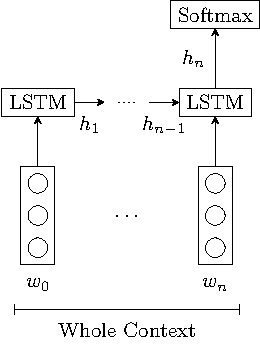
\includegraphics{Diagrams/Reproducibility/tang_lstm.pdf}
    \caption{Architecture of the LSTM method.}
    \label{fig:repro_lstm_method}
\end{figure}

The TDLSTM which can be seen in figure \ref{fig:repro_tdlstm_method}, is a target specific model, it splits the sentence into two contexts:
\begin{enumerate}
    \item Left context -- The words left of the target word, including the target itself.
    \item Right context -- The words right of the target word, including the target itself.
\end{enumerate}
Each context has its own LSTM, the left has an LSTM that takes words vectors from left to right, and the right LSTM takes words vectors from right to left. The last word vector(s) that are input into both LSTMs are the target words, this was so that the LSTM could better model the sentiment of the sentence with regard to the target word(s). The final output of both LSTMs ($h_{r-1}$, $h_{l+1}$) are concatenated together, which is fed into a linear layer with a softmax activation function to generate the probability of the sentiment of the text.

\begin{figure}[!h]
    \centering
    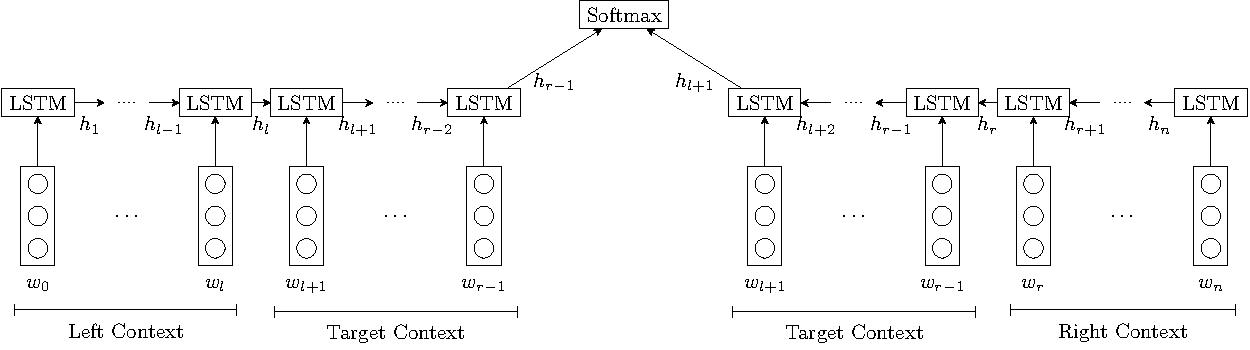
\includegraphics[scale=0.55]{Diagrams/Reproducibility/tang_tdlstm.pdf}
    \caption{Architecture of the TDLSTM method.}
    \label{fig:repro_tdlstm_method}
\end{figure}

Finally the TCLSTM method which can be seen in figure \ref{fig:repro_tclstm_method} is a direct extension of TDLSTM with only one minor difference. The difference is the concatenation of the target word vector ($t$) to each word vector within the text. The target word vector is represented as the average of all the target word vectors when the target word is made up of more than one word.

\begin{figure}[!h]
    \centering
    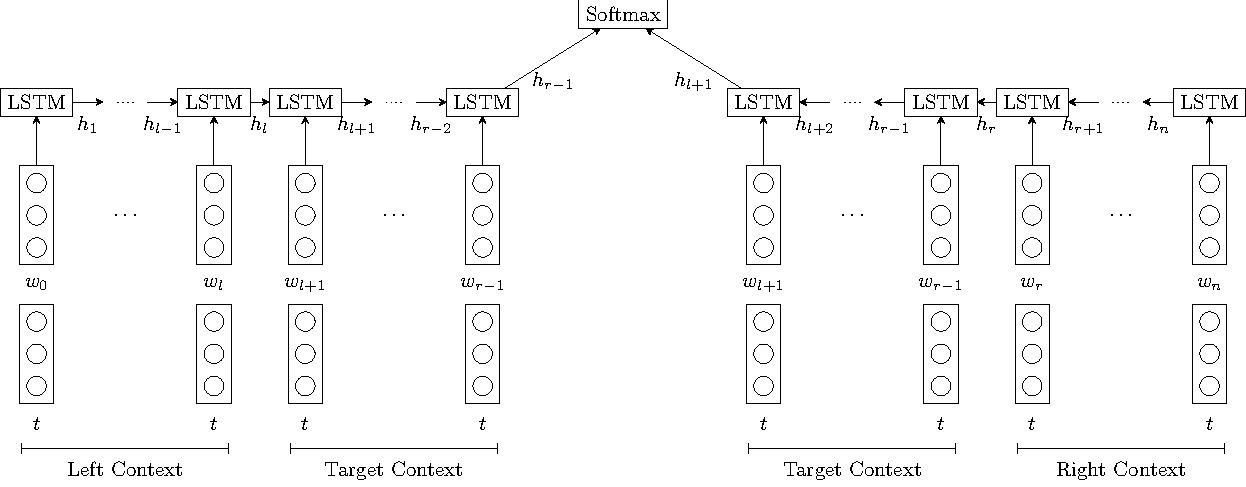
\includegraphics[scale=0.55]{Diagrams/Reproducibility/tang_tclstm.pdf}
    \caption{Architecture of the TCLSTM method.}
    \label{fig:repro_tclstm_method}
\end{figure}

%\subsection{Review of the three methods}
%The reason these three methods were chosen is two fold; first they can be split by the classifier the method uses, either a linear SVM or non linear NN, of which even though they have been compared before \cite{tang-etal-2016-effective, wang-etal-2017-tdparse} they have not been compared on datasets that are not Twitter based. Secondly \citet{vo2015target} and \citet{wang-etal-2017-tdparse} are very similar with the only difference being the whole and dependency contexts therefore it would be interesting to see if the dependency context is of importance generally across datasets that are not Twitter based.


\section{TDSA Reproduction Studies}
\label{section:repro_replication}

These studies will explore how the results from the original methods differ with those reproduced. Each paper will have its own subsection detailing the differences and if the differences are statistically significant. Furthermore, at the end of the section based on the results, suggestions are offered to make papers more reproducible. Lastly based on the reproduction results of \citet{tang-etal-2016-effective} additional suggestions are made for NN based methods to improve reporting of results, which in itself helps with both evaluation and reproducibility. A paper is defined as being reproduced if the main result is not statistically significantly different on at least one metric and if the results have the same rank order e.g. model A is better than model B for at least one metric. In the thesis, this is how the definition for reproducibility from the introduction \ref{section:repro_intro} has been empirically interpreted. Before conducting the reproducibility studies, the experimental setup for all of these studies will be stated defining the metrics, datasets, pre-processing steps, and how the statistical significance tests will be performed.

%The replication cases here will show that the methods recreated within this thesis can successfully replicate the experiments conducted within the papers of the three methods stated in section \ref{section:repro_methods}. The success is shown through the replicated methods to be not statistically different to the original methods on at least one of the metrics used. The importance of having accurately replicated methods is to allow the findings within the mass evaluation \ref{section:repro_mass_eval} and effects of parameter and experimental settings \ref{section:repro_effect_param_settings} sections to be valid and representative of the original method. This section will first explain how the experiments are setup and iteratively go through each of the three methods demonstrating that each has been successfully replicated.

%This section will demonstrate that the three methods stated above in the methods section \ref{section:repro_methods} are successfully replicated using significance testing. The section will start with a description of the significance test used in all the experiments, followed by a experiment(s) for each of the three methods to show that the methods have been successfully replicated.

%We now demonstrate through replicating the experiments in each paper and using statistical test that we have successfully replicated all of the methods.\\

% This might be better placed in the generlisation section/ dataset explaination section.
%
% This in itself is a bad dataset to be used for TDSA as there is only one unique target per sentence which can be seen in table \ref{table:repro_datasets_stats}. Even though the sentiment is with respect to the target and not the sentence you would not get issues such as conflicting sentiments within the sentence due to different targets having different sentiment. For example `The camera is very good but the lens is awful' would have two targets with conflicting sentiments.\\
% Type I error refers to the case where the null hypothesis is rejected when it is actually true. Type II error refers to the case where the null hypothesis is not rejected although it should be. A

%The methods within this subsection all use the general domain Twitter dataset from \cite{dong-etal-2014-adaptive}, \cite{wang-etal-2017-tdparse} also used their own political Twitter dataset. The pre-processing across all of the experiments is the same. We follow \cite{vo2015target} which is to lower case all text and tokenise using Twokenizer \cite{gimpel-etal-2011-part}. This process was used as the other papers do not explicitly state their pre-processing method. Furthermore the word embeddings used in all of the tests only contain lower cased words and the Twokenizer tokeniser is Twitter specific, thus justifying this pre-processing method.
\subsection{Experimental Setup}
\label{section:repro_experimental_setup}

Within the reproduction and mass evaluation experiments the following datasets will be used: 

\begin{enumerate}
    \item Laptop -- SemEval 2014 laptop dataset \citep{pontiki-etal-2014-semeval}.
    \item Restaurant -- SemEval 2014 restaurant dataset \citep{pontiki-etal-2014-semeval}.
    \item Mitchell -- English Twitter dataset \citep{mitchell-etal-2013-open}\footnote{The reason for specifying English is due to \citet{mitchell-etal-2013-open} also releasing a Spanish Twitter dataset within the same paper.}.
    \item Dong -- Twitter dataset \citep{dong-etal-2014-adaptive}.
    \item Election -- Election Twitter dataset \citep{wang-etal-2017-tdparse}.
    \item YouTuBean -- Captions from YouTube review videos \citep{marrese-taylor-etal-2017-mining}.
\end{enumerate}

Table \ref{table:repro_dataset_stats} provides a description of the datasets, of which the YouTuBean is by far the smallest dataset. The sentiment class and Distinct Sentiment (\textit{DS}) distributions can be seen in table \ref{table:repro_dataset_sent_dist}. The \textit{DS} \citep{wang-etal-2017-tdparse} is based around the number of unique sentiments per text: $DS_1$, $DS_2$, and $DS_3$ would be all the samples that contain only one, two, and three sentiments in the text, respectively. The idea behind showing the \textit{DS} is a way of judging potentially how difficult a dataset is going to be where the larger $i$ in $DS_i$ the more difficult the dataset might be\footnote{In chapter \ref{chapter:methodology} it is shown empirically that the large $i$ is within $DS_i$ the more difficult it will be to classify the samples within that distribution.}. Thus from both tables it is clear to see that the datasets are all very different with some being heavily unbalanced with respect to sentiment class distribution, like the Mitchell dataset.

\begin{table}[!h]
    \centering
    \begin{tabular}{|c|c|c|c|c|c|c|c|}
\hline
Dataset & DO & T & M & No. Targets & ATS & Uniq & AVG Len \\
 \hline
Laptop & L & RE & W & 2951 & 1.58 & 1295 & 18.57  \\
\hline
Restaurant & R & RE & W & 4722 & 1.83 & 1630 & 17.25  \\
\hline
Mitchell & G & S & W & 3288 & 1.22 & 2507 & 18.02 \\
\hline
Dong & G & S & W & 6940 & 1.00 & 145 & 17.37 \\
\hline
Election & P & S & W & 11899 & 2.94 & 2190 & 21.68 \\
\hline
YouTuBean & MP & RE\slash S & SP & 798 & 2.07 & 522 & 22.53 \\
\hline
\multicolumn{8}{|p{0.95\linewidth}|}{L=Laptop, R=Restaurant, P=Politics, MP=Mobile Phones, G=General, T=Type, RE=Review, S=Social Media, ATS=Average targets per sentence, Uniq=No. unique targets, AVG len=Average sentence length per target, DO=Domain, M=Medium, W=Written, SP=Spoken}\\
\hline
\end{tabular}
    \caption{Dataset descriptions and size statistics.}
    \label{table:repro_dataset_stats}
\end{table}

\begin{table}[!h]
    \centering
    \begin{tabular}{|c|c|c|c|c|c|c|}
        \hline
        Dataset & Pos \sd{(\%)} & Neu \sd{(\%)} & Neg \sd{(\%)} & $DS_1$ & $DS_2$ & $DS_3$ \\
        \hline
        Laptop & 1328 \sd{(45)} & 629 \sd{(21.3)} & 994 \sd{(33.7)} & 81\% & 18\% & 1\% \\
        \hline
        Restaurant & 2892 \sd{(61.3)} & 829 \sd{(17.6)} & 1001 \sd{(21.2)} & 75\% & 23\% & 2\% \\
        \hline
        Mitchell & 707 \sd{(21.5)} & 2306 \sd{(70.1)} & 275 \sd{(8.4)} & 91\% & 9\% & 0\% \\
        \hline
        Dong & 1734 \sd{(25)} & 3473 \sd{(50)} & 1733 \sd{(25)} & 100\% & 0\% & 0\% \\
        \hline 
        Election & 1744 \sd{(14.7)} & 4572 \sd{(38.4)} & 5583 \sd{(46.9)} & 44\% & 47\% & 9\% \\
        \hline 
        YouTuBean & 224 \sd{(28.1)} & 504 \sd{(63.2)} & 70 \sd{(8.8)} & 82\% & 18\% & 0\% \\
        \hline
        \multicolumn{7}{|p{0.85\linewidth}|}{Pos=Number of positive targets, Neu=Number of neutral targets, Neg=Number of negative targets, $DS_1$=1 Distinct Sentiment per sentence, $DS_2$=2 Distinct Sentiments per sentence, $DS_3$=3 Distinct Sentiments per sentence}\\
        \hline
\end{tabular}
    \caption{Dataset sentiment class and distinct sentiment distributions.}
    \label{table:repro_dataset_sent_dist}
\end{table}

The Dong dataset\footnote{This dataset can be downloaded from \url{http://goo.gl/5Enpu7}.} is a special case out of all of the datasets, as even though it has been used in previous research as shown in table \ref{table:repro_methods_datasets_used}, it is not a true TDSA dataset. The dataset is more of an Aspect Based Sentiment Analysis dataset as the annotation gives the target and all of its occurrences in the text, rather than just the relevant target occurrence. Example \ref{example:repro_dong_data_example} is from the training dataset, where \$T\$ represents all of the places the target occurs in the text, and here it is clear that the first target (\$T\$) is not the target that is negatively affected rather it is the second target (\$T\$). This issue of not knowing which is the relevant target was denoted as ``same target multiple appearances'' by \citet{wang-etal-2017-tdparse}. Thus when using the Dong dataset for the \citet{tang-etal-2016-effective} methods the first target (\$T\$) is assumed to be the relevant target in all cases, and when using the NP approaches the feature vector of all target occurrences are median pooled which is the approach used by \citet{wang-etal-2017-tdparse}. It is not clear how either \citet{vo2015target} or \citet{tang-etal-2016-effective} handled the `same target multiple appearance' issue.

\begin{example}
\textit{\$T\$ has brought back the female rapper . - really ? \$T\$ is the biggest parody in popular music since the Lonely Island .}
\caption{An example from the training dataset of Dong \citep{dong-etal-2014-adaptive}, where \$T\$ is a placeholder for the target `nicki minaj'. The sentiment towards the target is negative.}
\label{example:repro_dong_data_example}
\end{example}

As stated earlier, to test if the method has been successfully reproduced the results from the reproduced method will not be statistically significantly different to the original method's results. To choose an appropriate statistical test, the guide from \citet{dror-etal-2018-hitchhikers} has been followed, from which the non-parametric paired bootstrap test \citep{efron_1993} has been selected. This was chosen as the distribution of results cannot always be assumed to come from a normal distribution, due to the macro F1 metric \citep{dror-etal-2018-hitchhikers} which is one of the metrics used within the experiments. Thus this breaks the assumptions of the more powerful parametric tests (student's t-test). Furthermore, out of the two families of non-parametric tests the sampling-based tests are more powerful \citep{dror-etal-2018-hitchhikers, sogaard-etal-2014-whats} (fewer type 2 errors\footnote{Type 2 error: `refers to the case where the null hypothesis is not rejected although it should be.'\citep{dror-etal-2018-hitchhikers}}), from this either Pitman's permutation test or the paired bootstrap can be used, thus we follow \citet{sogaard-etal-2014-whats} in using the paired bootstrap test. The one assumption that has to be made with the paired bootstrap is that the test data is representative of the overall population by having a large enough test set size. Therefore we take the suggestion from \citet{sogaard-etal-2014-whats} and assume that a test set of size greater than 200 is enough to ensure the type 1 errors\footnote{Type 1 error: `refers to the case where the null hypothesis is rejected when it is actually true.'\citep{dror-etal-2018-hitchhikers}} are minimised. The only experiments that cannot assume the test size is greater than 200 are those that apply five-fold cross validation on the YouTuBean dataset.

%For one of the metrics (accuracy) it can be assumed that the results have come from a normal distribution \citep{dror-etal-2018-hitchhikers}. However as the number of results created from the NP methods when evaluated purely on the test sets will be one, one result is not a distribution of results. Thus for any of the parametric tests to work a large enough sample of results is needed, which is at least greater than one. Hence another reason why the parametric tests cannot be used even for results that come from a metric that can be assumed to come from a normal distribution, like in this case accuracy.

%To further explain why our results will not follow a normal distribution, this is due to the two metrics that are used through out most of the experiments. The two metrics are the macro F1 score and accuracy, results from the accuracy metric can be assumed to be normal if the number of predictions is large enough \citep{dror-etal-2018-hitchhikers}. However considering the minimum number of scores produced for each experiment will be 1 this would not be considered `large enough' thus a normal distribution cannot be assumed for the accuracy metric. %Also within the reproduction case of \citet{tang-etal-2016-effective} it is shown by using the Shapiro-Wilk test \citep{shapiro1965analysis} for normality (which is the recommended test within \citet{dror-etal-2018-hitchhikers}) that not all accuracy metric scores come from a normal distribution. Thus as it cannot be assumed that all accuracy scores come from a normal distribution and F1 scores have not be shown too either, we assume the results will not follow a normal distribution.

The metrics used in all the experiments will be both the accuracy and macro F1 scores as these are the most frequently used metrics within TDSA \citep{dong-etal-2014-adaptive,wang-etal-2017-tdparse,he-etal-2018-exploiting}. The accuracy score can be calculated using equation \ref{eq:repro_accuracy} where $TP$ refers to the number of correctly labelled samples and $N$ are the number of samples in the dataset. The macro F1 score can be calculated using equation \ref{eq:repro_macro_f1} where the $F1(pos)$, $F1(neu)$, and $F1(neg)$ is the F1 score for the positive, neutral, and negative classes respectively. One of the differences between the two is that the accuracy score is performed globally and thus does not discriminate based on the class label, whereas the macro F1 does as it has to calculate the F1 score for each class and then perform an un-weighted average across all three classes. Due to the un-balanced nature of class labels within all of the TDSA datasets, as shown in table \ref{table:repro_dataset_sent_dist}, the macro F1 score is more biased towards methods that perform well across all sentiments rather than just the dominant sentiment. In comparison, the accuracy score can still be very high with just predicting the most dominant sentiment all of the time. Finally, the majority baseline for accuracy will always be greater than that of the macro F1 due to the un-weighted averaging over the sentiment classes. Thus in general the macro F1 score is a harder metric. The two metrics allow for fair comparison with other works in the community.

\begin{equation}
    Accuracy = \frac{TP}{N}
    \label{eq:repro_accuracy}
\end{equation}
\begin{equation}
    F1 = 2 * \frac{Recall * Precision}{Recall + Precision}
\end{equation}
\begin{equation}
    Macro\, F1 = \frac{F1(pos)\, +\, F1(neu)\, + \, F1(neg)}{3}
    \label{eq:repro_macro_f1}
\end{equation}

The null hypothesis that is being tested within this reproduction section is the following: 
\begin{hyp}
The reproduced method (R) is no better or worse than the original method (O) on a given population x\footnote{x is defined later on in this section.}. 
\label{hyp:repro_replication_null}
\end{hyp}
While the alternative is:
\begin{hyp}
The reproduced method (R) is better or worse than the original method (O) on a given population x. 
\label{hyp:repro_replication_alt}
\end{hyp}
The null hypothesis \ref{hyp:repro_replication_null} will be tested using a two tailed test as it is to be seen if the reproduced method is better or worse rather than just one of those options otherwise a one tailed test would be used. This null hypothesis can be expressed through equations \ref{eq:repro_null_hypo_better}\footnote{X is defined later on in this section.} and \ref{eq:repro_null_hypo_worse}, where $\delta(x)$ is expressed in equation \ref{eq:repro_score_diff} and $M$ represents an evaluation metric of which this would be either accuracy or macro F1.

\begin{equation}
    p(\delta(X\footnote{X is defined later on in this section.}) \leq 0)
\label{eq:repro_null_hypo_better}
\end{equation}

\begin{equation}
    p(\delta(X) \geq 0)
\label{eq:repro_null_hypo_worse}
\end{equation}

\begin{equation}
    \delta(x) = M(R(x)) - M(O(x))
\label{eq:repro_score_diff}
\end{equation}

To reject the null hypothesis \ref{hyp:repro_replication_null} and accept the alternative hypothesis \ref{hyp:repro_replication_alt} equation \ref{eq:repro_null_diff_better} or \ref{eq:repro_null_diff_worse} has to be true for some given $\alpha$.
\begin{equation}
    p(\delta(X) \leq 0) \le \frac{\alpha}{2}
\label{eq:repro_null_diff_better}
\end{equation}
\begin{equation}
    p(\delta(X) \geq 0) \le \frac{\alpha}{2}
\label{eq:repro_null_diff_worse}
\end{equation}
The $\alpha$ value\footnote{It is suggested in \citet{sogaard-etal-2014-whats} that an $\alpha$ of 0.0025 should be used and that p-values are recorded.} determines the upper bound on the number of type 1 errors that can occur \citep{dror-etal-2018-hitchhikers}. Therefore in this thesis an $\alpha$ value of 0.05 is chosen as this is the most popular value used within the field \citep{liu-zhang-2017-attention,he-etal-2018-exploiting}.

The population $x$ is normally our test set when comparing two systems, and we assume that this test has come from a large population $X$. The null hypothesis is used to ensure that our one test score on the given test set $x$ has not come about by chance. Therefore to compute the p-value for equations \ref{eq:repro_null_hypo_better} and \ref{eq:repro_null_hypo_worse} we approximate the larger population $X$ using the bootstrap re-sampling method. This is a method of creating $Z$ test sets of size $n$, which is the same size as the original test set, by sampling from the original test set with replacement. The assumption is that this creates new test sets that are representative but different from the original, which can be used as a proxy of the larger population $X$. The paired bootstrap procedure is presented in algorithm \ref{algo:repro_bootstrap}, which is used to approximate the p-values of which $p_0$ and $p_1$ can be substituted as the p-value in equations \ref{eq:repro_null_diff_better} and \ref{eq:repro_null_diff_worse}. For all experiments $Z$ is at least equal to 1000\footnote{In some cases where it was computationally feasible $Z$ was 10,000.}, which is the same as \citet{koehn-2004-statistical} used and is computationally feasible. 

\begin{algorithm}
    Draw \textit{Z} bootstrap samples of size $n$ by sampling with replacements from $x$\;
    $w = 0$\;
    $b = 0$\;
    \For{each $x^{(i)}$ increment}{
        \uIf{$\delta(x^{(i)}) < 0$}
        {
            $w = w + 1$\;
        }
        \uIf{$\delta(x^{(i)}) > 0$}
        {
            $b = b + 1$\;
        }
    }
    $p_0$ $\approx 1 - \frac{w}{Z}$\;
    $p_1$ $\approx 1 - \frac{b}{Z}$\;
    return $p_0$ and $p_1$\;
    \caption{The paired bootstrap algorithm adapted from figure 1 in \citet{berg-kirkpatrick-etal-2012-empirical}}
    \label{algo:repro_bootstrap}
\end{algorithm}

This bootstrapping approach can therefore be used to create a confidence range for a method whereby using these $Z$ metric scores as a distribution of results. From this distribution removing the top and bottom 2.5\% of scores creates the confidence range for an $\alpha=0.05$\footnote{The percentage to remove is equal to $\frac{\alpha}{2} \times 100$ for the two tailed test.}, for the two tailed test, as shown by \citet{koehn-2004-statistical}. If the reproduced confidence range does not include the original method's score the null hypothesis must be rejected. 

The two tailed test can easily be converted into a one tailed test, to test if a method is better than another, whereby the hypothesis now changes to:
\begin{hyp}
Reproduced method A is no better than the original method B on a given population x. 
\label{hyp:repro_replication_better_null}
\end{hyp}
While the alternative is:
\begin{hyp}
Reproduced method A is better than the original method B on a given population x. 
\label{hyp:repro_replication_better_alt}
\end{hyp}

The null hypothesis \ref{hyp:repro_replication_better_null} can be expressed by equations \ref{eq:repro_null_hypo_worse} and \ref{eq:repro_score_better_diff}.  

\begin{equation}
 \delta(x) = M(A(x)) - M(B(x))
\label{eq:repro_score_better_diff}
\end{equation}

To reject this null hypothesis \ref{hyp:repro_replication_better_null} equation \ref{eq:repro_null_diff_better_worse} has to be true for some $\alpha$, which in this thesis is $0.05$. 
\begin{equation}
    p(\delta(X) \geq 0) \le \alpha
\label{eq:repro_null_diff_better_worse}
\end{equation}

The pre-processing for the two NP approaches will use the Twitter based tokeniser; Twokenizer \citep{gimpel-etal-2011-part} as this was stated within \citet{vo2015target} and is shown to be used within \citet{wang-etal-2017-tdparse} codebase\footnote{\url{https://github.com/bluemonk482/tdparse/blob/master/data/dataprocessing.py}}. For the LSTM approach \citep{tang-etal-2016-effective} the English Spacy tokeniser is used due to its speed and wide use within the NLP field, as well as \citet{tang-etal-2016-effective} not stating the tokeniser used. All text is lower cased after being tokenised.

For the NP methods, scikit-learn's \citep{pedregosa2011scikit} LinearSVC is used as it is a wrapper of LibLinear \citep{fan2008liblinear} which is the library that both NP papers used for their SVMs. For \citet{tang-etal-2016-effective} LSTM based methods the AllenNLP framework \citep{gardner-etal-2018-allennlp} is used which uses PyTorch \citep{NEURIPS2019_9015}. 



\subsection{Neural Pooling}
\label{section:repro_neural_pooling}
To state if the paper \citep{vo2015target} has been reproduced the last experiment in the paper (table 5 \citep{vo2015target}) is performed which evaluates the methods on the test set of \citet{dong-etal-2014-adaptive} Twitter dataset. To be comparable the same SVM C-value parameters are used for all methods and sentiment lexicons for the Target-Dependent Plus method. Also the same word vectors are used which are the concatenation of the unified Sentiment Specific Word Embeddings (SSWE) \citep{tang-etal-2014-learning} and their own Twitter specific continuous skip-gram \citep{mikolov2013efficient} word vectors (w2v) creating SSWE + w2v. Finally MinMax scaling, as shown in equation \ref{eq:repro_min_max_scaling}, is used on all features, whereby this enforces a feature to be in a pre-defined \textit{max} to \textit{min} range for all samples ($X \in \R^{n \times d}$ where $n$ is the number of samples and $d$ is the number of features). This therefore enforces all features to be within the same range and ``avoid attributes (features) in greater numeric ranges dominating those in smaller numeric ranges'' \citep{hsu2003practical}. $X_{min} \in \R^d$ and $X_{max} \in \R^d$ are the smallest and largest value respectively for each feature. Within this thesis the \textit{min} and \textit{max} will be $0$ and $1$ respectively as this is one of the recommended ranges by \citet{hsu2003practical}. Only after the experiments have been conducted within this thesis, after looking through \citet{wang-etal-2017-tdparse} codebase, was it found they used $-1$ and $1$ for \textit{min} and \textit{max}. Thus it will be shown the difference between using these two different \textit{min} and \textit{max} ranges is negligible.

\begin{equation}
    X = \frac{X - X_{min}}{X_{max} - X_{min}} * (max - min) + min
    \label{eq:repro_min_max_scaling}
\end{equation}

The results from this experiment can be seen in table \ref{table:repro_vo_main_results} which compares the reproduced to the original. The original did not use the Target-Dependent Minus method within this experiment. As can be seen the results are similar to the original. However by adding only target context information and removing the whole text context (Target-Dependent Minus) does not improve results greatly over the standard non-target aware method (Target-Independent). Further Target-Dependent Minus is not statistically significantly better than Target-Independent on either of the two metrics, as shown by the p-values in table \ref{table:repro_vo_main_results_p_values}. Thus showing for the first time that adding the whole text context is statistically significant within the Target-Dependent method and not just on average better, as shown by table \ref{table:repro_vo_main_results_p_values}. Figure \ref{fig:repro_vo_Target_Reproduction_Dong} shows the confidence intervals of each reproduced method, and that for the accuracy metric all of the original results are within confidence intervals. Further according to the results all methods are in the same rank order as the original. Thus this paper has been reproduced.

\FloatBarrier
\begin{table}[!h]
    \centering
    \begin{tabular}{|c|c|c|c|c|}
 \hline
 & \multicolumn{2}{c|}{Accuracy} & \multicolumn{2}{c|}{macro F1} \\
 \hline
 Model & O & R & O & R \\ 
 \hline
 Target Independent     &     67.3 &         65.0 &     66.4 &         61.9 \\
 \hline
 Target Dependent Minus &      0.0 &         66.6 &      0.0 &         62.1 \\
 \hline
 Target Dependent       &     69.7 &         69.7 &     68.0 &         66.7 \\
 \hline
 Target Dependent Plus  &     71.1 &         69.9 &     69.9 &         67.6 \\
\hline
\end{tabular}
    \caption{Reproduced (R) and original (O) results on the test set of \citet{dong-etal-2014-adaptive} Twitter dataset.}
    \label{table:repro_vo_main_results}
\end{table}
\FloatBarrier

\FloatBarrier
\begin{table}[!h]
    \centering
    \begin{tabular}{|c|c|c|c|c|c|}         
\hline
Metric &    Method                   &  TI &  TDM &  TD &  TDP \\
\hline
\multirow{4}{*}{macro F1} & TI &              - &                  0.5459 &            0.9976 &                 0.9995 \\
& TDM &              0.4541 &                  - &            0.9995 &                 0.9994 \\
& TD &              \textbf{0.0024} &                  \textbf{0.0005} &            - &                 0.7606 \\
& TDP &              \textbf{0.0005} &                  \textbf{0.0006} &            0.2394 &                 - \\
\hline
\multirow{4}{*}{Accuracy} & TI &              - &                  0.8245 &            0.9987 &                 0.9986 \\
& TDM &              0.1962 &                  - &            0.9935 &                 0.9905 \\
& TD &              \textbf{0.0017} &                  \textbf{0.0094} &            - &                 0.6284 \\
& TDP &              \textbf{0.0019} &                  \textbf{0.0121} &            0.4223 &                 - \\
\hline
\end{tabular}
    \caption{P-values testing if the methods in the rows are significantly better than the methods in the columns across two metrics. All p-values that are significant $\le 0.05$ are in \textbf{bold}.}
    \label{table:repro_vo_main_results_p_values}
\end{table}
\FloatBarrier

\begin{figure}[!h]
    \centering
    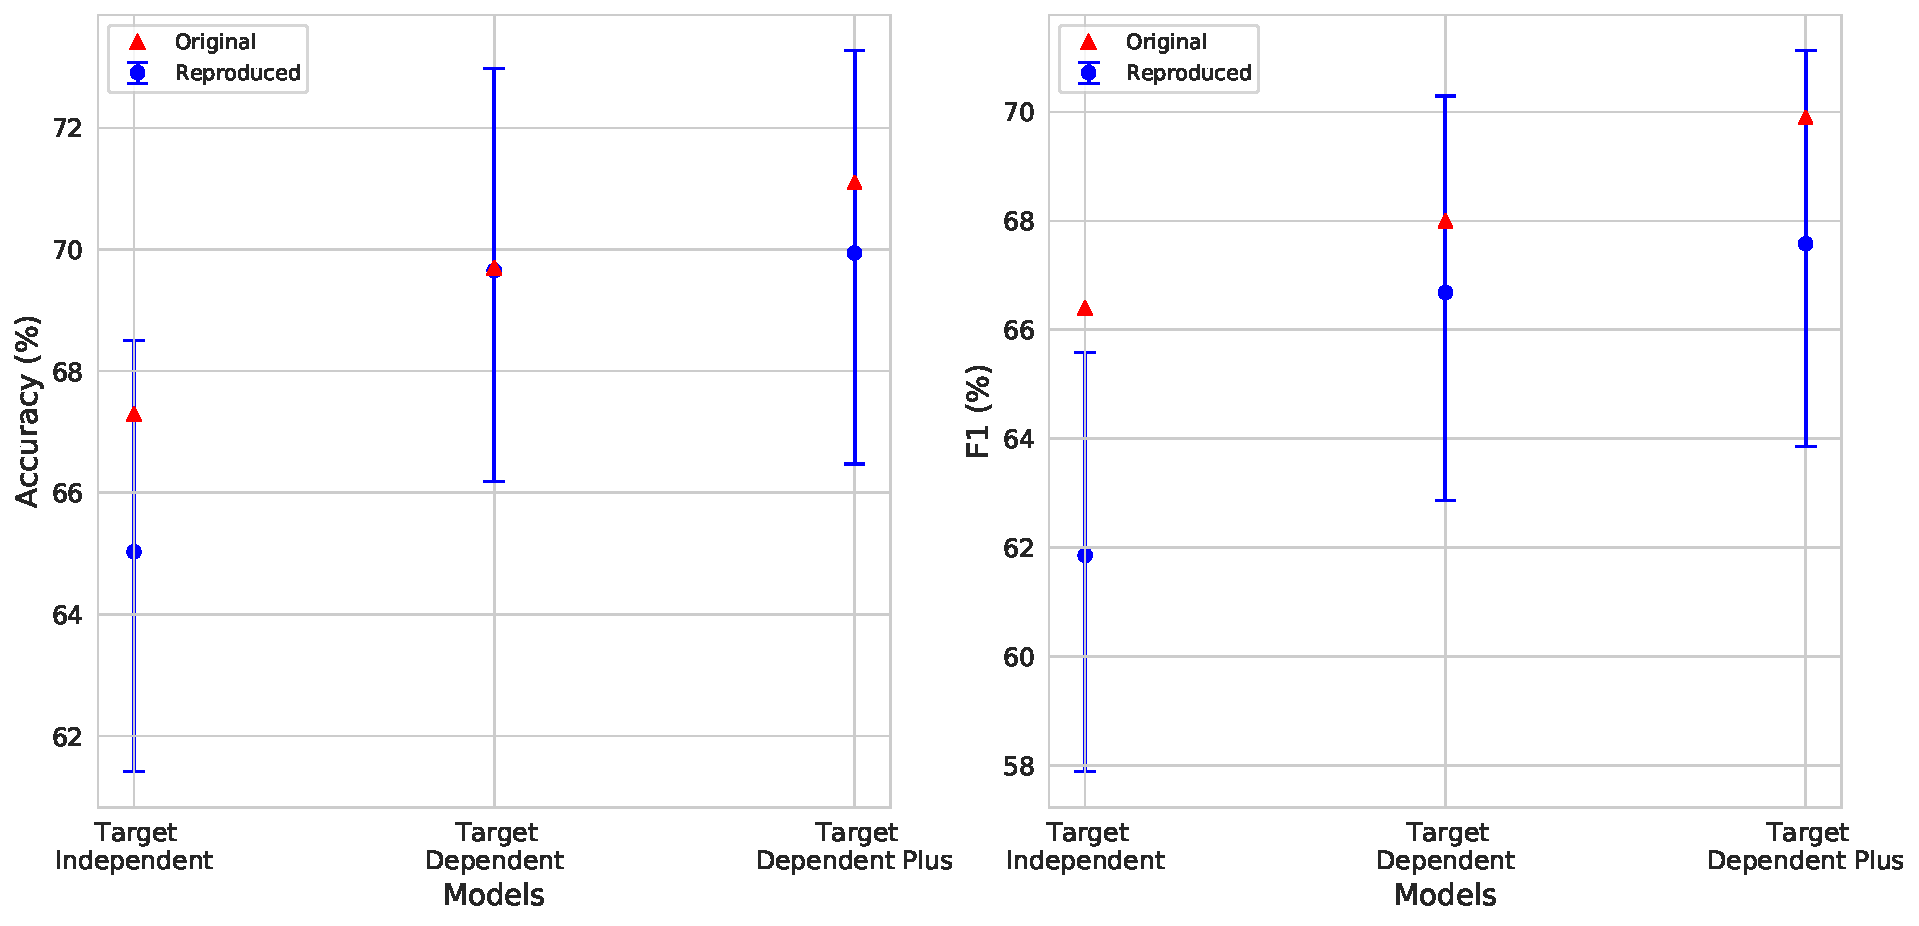
\includegraphics[scale=0.37]{images/reproducibility/vo/Target_Reproduction_Dong.pdf}
    \caption{Confidence intervals for the two tailed test for the reproduced models of \citet{vo2015target} on both the accuracy and macro F1 metrics.}
    \label{fig:repro_vo_Target_Reproduction_Dong}
\end{figure}

As stated earlier \citet{wang-etal-2017-tdparse} used a different scaling range, $-1$ to $1$, for MinMax scaling. Figure \ref{fig:repro_vo_Target_Wang_Scaled_Reproduction_Dong} shows the confidence intervals for each method when using \citet{wang-etal-2017-tdparse} scaling range on the test set of \citet{dong-etal-2014-adaptive} Twitter dataset. As can be seen the confidence intervals would overlap with those from figure \ref{fig:repro_vo_Target_Reproduction_Dong} which used the $0$ to $1$ scaling range that is used throughout the Neural Pooling experiments. Thus showing in this case the scaling range would not appear to be a significant factor.

\begin{figure}[!h]
    \centering
    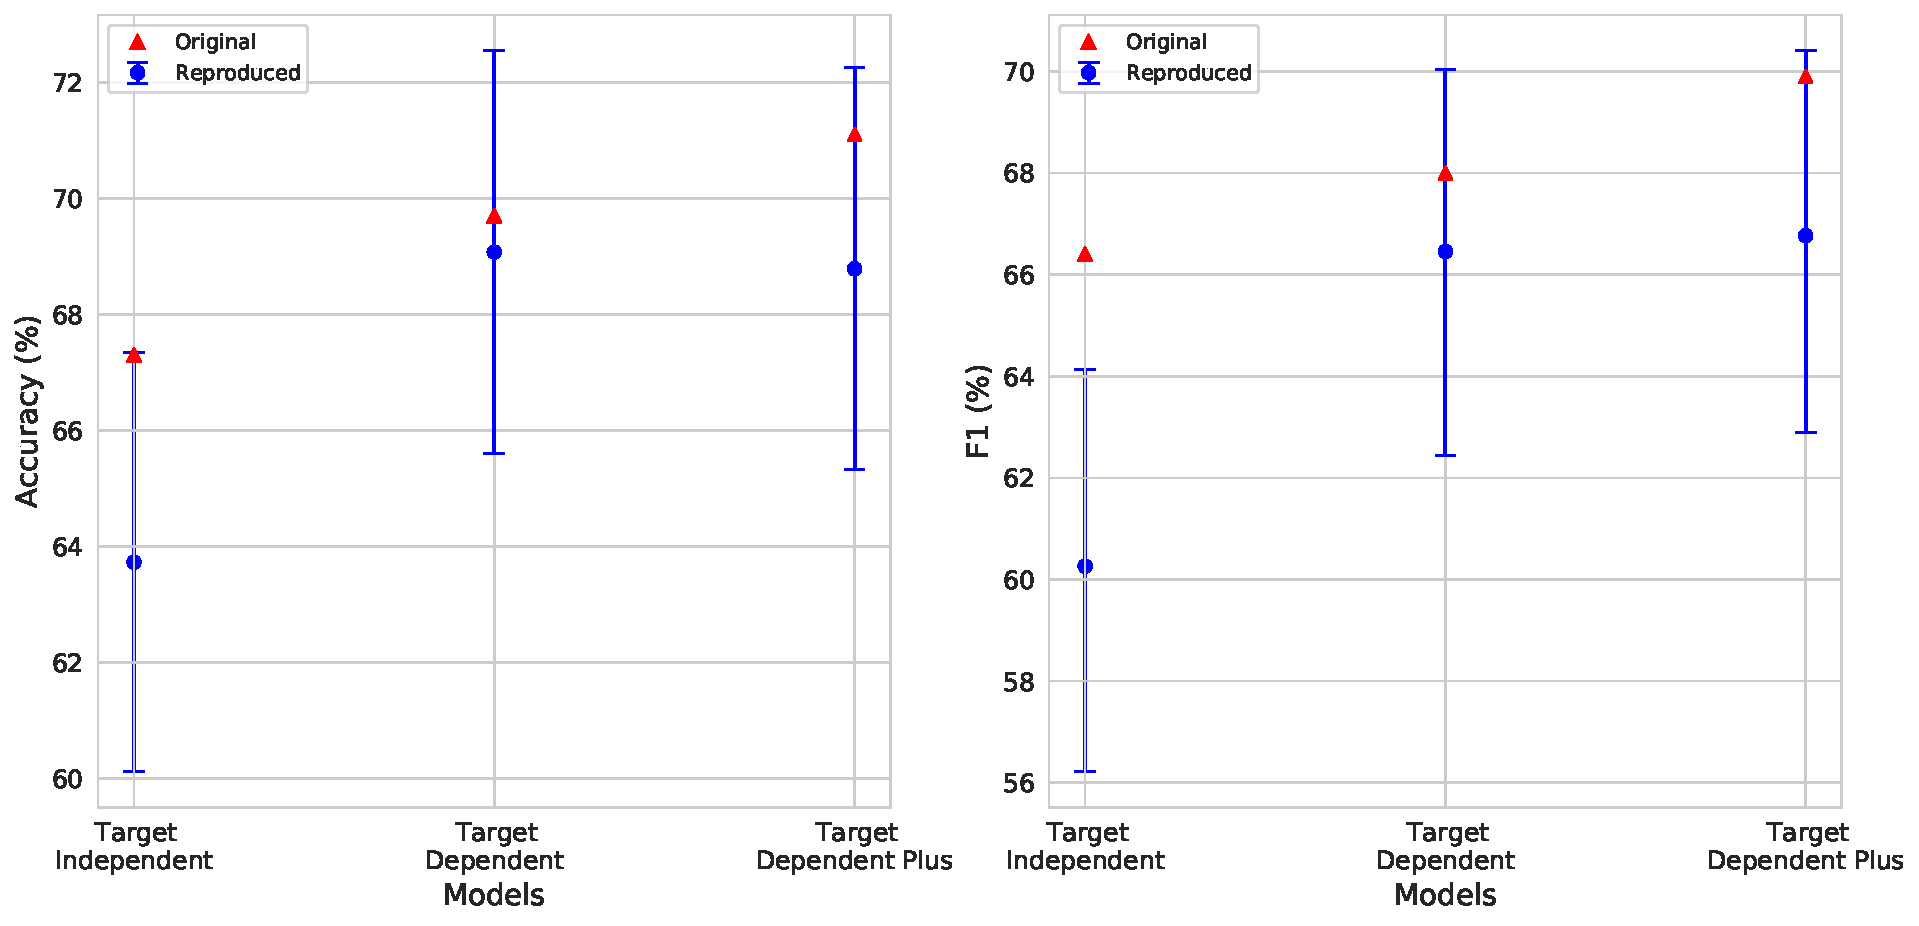
\includegraphics[scale=0.37]{images/reproducibility/vo/Target_Wang_Scaled_Reproduction_Dong.pdf}
    \caption{Confidence intervals for the two tailed test for the reproduced models of \citet{vo2015target} using \citet{wang-etal-2017-tdparse} scaling range of $-1$ to $1$, on both the accuracy and macro F1 metrics.}
    \label{fig:repro_vo_Target_Wang_Scaled_Reproduction_Dong}
\end{figure}

Given that the paper has been reproduced, further studies are explored. The first of which is comparing different word embeddings, in \citet{vo2015target} they compared w2v, SSWE, and SSWE + w2v. The comparison was done using five-fold cross validation on the training data whereby they report the mean accuracy scores within figure 4 of their paper. This experiment has been recreated, and the word embeddings compared have been expanded to include the non-type non-task specific 300 dimension 840 billion token GloVe embeddings \citep{pennington-etal-2014-glove} (from now on called GloVe embeddings). These much larger word embeddings are by the far the most popular embeddings within the TDSA literature. Furthermore unlike w2v which are type specific and SSWE which are task and type specific these are neither and more general. Thus it would be of interest to see if general embeddings can perform as well or better than the original task and type specific embeddings. The results of the experiment can be seen in table \ref{table:repro_vo_word_embeddings_results}. As can be seen the GloVe and the SSWE + w2v are very similar in their performance, and both always outperform the w2v and SSWE embeddings. However unlike the original results, the reproduced results tend to find w2v to perform better than SSWE, as shown by the highlighting in the table.  

\FloatBarrier
\begin{table}[!h]
    \centering
    \begin{tabular}{|c|c|M|M|c|M|}
\hline
&  & \multicolumn{2}{c|}{Accuracy} & \multicolumn{2}{c|}{macro F1} \\
\hline
Method & Embedding &      O &  R &     O &  R \\
\hline
\multirow{4}{*}{TI} & w2v &  59.20 \sd{(0.00)} &  \highbox{60.96} \sd{(0.60)} &  - &  56.64 \sd{(0.69)} \\
& SSWE &  60.70 \sd{(0.00)} &  \highbox{60.58} \sd{(1.08)} &  - &  56.52 \sd{(1.46)} \\
& SSWE + w2v &  62.30 \sd{(0.00)} &  62.24 \sd{(0.91)} &  - &  59.16 \sd{(0.66)} \\
& GloVe &   - &  \textbf{63.72} \sd{(1.76)} &  - &  \textbf{61.31} \sd{(1.74)} \\
\hline
\multirow{4}{*}{TDM} & w2v &  65.40 \sd{(0.00)} &  65.67 \sd{(1.11)} &  - &  61.38 \sd{(1.29)} \\
& SSWE &  66.60 \sd{(0.00)} &  66.74 \sd{(0.48)} &  - &  62.77 \sd{(0.78)} \\
& SSWE + w2v &  67.60 \sd{(0.00)} &  \textbf{67.46} \sd{(1.04)} &  - &  \textbf{64.18} \sd{(1.18)} \\
& GloVe &   - &  67.41 \sd{(0.78)} &  - &  64.11 \sd{(0.82)} \\
\hline
\multirow{4}{*}{TD} & w2v &  65.70 \sd{(0.00)} &  \highbox{66.81} \sd{(0.86)} &  - &  62.66 \sd{(1.16)} \\
& SSWE &  66.70 \sd{(0.00)} &  \highbox{66.37} \sd{(0.59)} &  - &  62.41 \sd{(0.81)} \\
& SSWE + w2v &  68.30 \sd{(0.00)} &  68.02 \sd{(0.82)} &  - &  64.90 \sd{(0.91)} \\
& GloVe &   - &  \textbf{68.69} \sd{(1.13)} &  - &  \textbf{65.68} \sd{(1.24)} \\
\hline
\multirow{4}{*}{TDP} & w2v &  67.40 \sd{(0.00)} &  \highbox{68.37} \sd{(1.17)} &  - &  65.04 \sd{(1.39)} \\
& SSWE &  67.90 \sd{(0.00)} &  \highbox{67.72} \sd{(1.11)} &  - &  64.39 \sd{(1.54)} \\
& SSWE + w2v &  69.10 \sd{(0.00)} &  \textbf{69.05} \sd{(1.19)} &  - &  66.34 \sd{(1.41)} \\
& GloVe &   - &  68.98 \sd{(1.09)} &  - &  \textbf{66.39} \sd{(1.23)} \\
\hline
\end{tabular}
    \caption{Mean (standard deviation) metric score for each method and embedding, where the \textbf{bold} value represents the best embedding for each method and metric. Difference in rank order is \highbox{highlighted}.}
    \label{table:repro_vo_word_embeddings_results}
\end{table}
\FloatBarrier

These results for the embedding comparison so far has only been based on mean accuracy scores from five-fold cross validation. To be more rigorous in evaluation, significant testing is performed whereby the one tailed test is performed on each fold comparing the SSWE + w2v embedding score per metric and method to all other embeddings. The SSWE + w2v embedding was compared to the others as this was the best embedding from the original paper. The p-values generated from these significant tests can be seen in appendix \ref{appendix_reproducibility_tables} tables \ref{table:repro_vo_appendix_embedding_p_values_accuracy} and \ref{table:repro_vo_appendix_embedding_p_values_macro_f1} for the accuracy and macro F1 scores respectively. Furthermore as the significance testing is now performed on five folds, which is equivalent to five datasets, thus creating five p-values for each evaluation. Therefore here the number of folds that are significant will be reported. However using the simple approach of counting the number of folds that are less than some $\alpha$ has been shown to introduce more type 1 errors \citep{dror-etal-2017-replicability} than that was set by the $\alpha$ parameter, which is $0.05$, in the individual significance tests. Therefore to stop the introduction of type 1 errors and keep the upper bound to $\alpha$ a correction procedure is required of which \citet{dror-etal-2018-hitchhikers} recommends two; Fisher and Bonferroni \citep{benjamini2008screening}. The difference between the two is that Fisher should be used when the p-values have come from datasets that are independent, where as Bonferroni can be used for dependent datasets. As each fold does depend on the other folds, the Bonferroni correction will be used here. This thus introduces how significance testing can be performed in general for multiple datasets.

Table \ref{table:repro_vo_word_embedding_sig_fold_count} shows that for at least one of the folds, metric, and methods SSWE + w2v is significantly better than the SSWE and w2v embeddings but not the GloVe. Thus showing like the original paper that SSWE + w2v are the best embedding in general out of SSWE and w2v. Furthermore the GloVe embedding is also tested to see if it is better than the other embeddings using a one sided test and corrected using Bonferroni\footnote{The p-values associated to these tests can be seen in appendix \ref{appendix_reproducibility_tables} tables \ref{table:repro_vo_appendix_embedding_glove_accuracy_p_values} and \ref{table:repro_vo_appendix_embedding_glove_f1_p_values} for the accuracy and macro F1 metrics respectively.}, of which the results can be seen in table \ref{table:repro_vo_glove_embedding_sig_fold_count}. Thus from both experiments in tables \ref{table:repro_vo_word_embedding_sig_fold_count} and \ref{table:repro_vo_glove_embedding_sig_fold_count} it shows that the GloVe embedding is a reasonable replacement for the type and task specific combination of SSWE + w2v.

\begin{table}[!h]
    \centering
    \begin{tabular}{|c|c|c|c|}
\hline
Method &    Embedding   &  Accuracy &  F1 \\
\hline
\multirow{3}{*}{Target Independent} & w2v &         0 &   2 \\
& SSWE &         1 &   2 \\
& GloVe &         0 &   0 \\
\hline
\multirow{3}{*}{Target Dependent Minus} & w2v &         3 &   4 \\
& SSWE &         0 &   0 \\
& GloVe &         0 &   0 \\
\hline
\multirow{3}{*}{Target Dependent} & w2v &         0 &   4 \\
& SSWE &         0 &   2 \\
& GloVe &         0 &   0 \\
\hline
\multirow{3}{*}{Target Dependent Plus} & w2v &         0 &   0 \\
& SSWE &         1 &   1 \\
& GloVe &         0 &   0 \\
\hline
\end{tabular}
    \caption{The number of folds, out of a possible of five, that the SSWE + w2v embedding is significantly better than the given embedding and method. The significant testing across multiple folds is corrected using Bonferroni.}
    \label{table:repro_vo_word_embedding_sig_fold_count}
\end{table}

\begin{table}[!h]
    \centering
    \begin{tabular}{|c|c|c|c|}
\hline
Method &    Embedding   &  Accuracy &  F1 \\
\hline
\multirow{3}{*}{Target Independent} & w2v &         2 &   5 \\
& SSWE &         1 &   5 \\
& SSWE + w2v &         1 &   1 \\
\hline
\multirow{3}{*}{Target Dependent Minus} & w2v &         0 &   1 \\
& SSWE &         0 &   1 \\
& SSWE + w2v &         0 &   0 \\
\hline
\multirow{3}{*}{Target Dependent} & w2v &         1 &   4 \\
& SSWE &         3 &   4 \\
& SSWE + w2v &         0 &   0 \\
\hline
\multirow{3}{*}{Target Dependent Plus} & w2v &         0 &   0 \\
& SSWE &         0 &   1 \\
& SSWE + w2v &         0 &   0 \\ 
\hline
\end{tabular}
    \caption{The number of folds, out of a possible of five, that the GloVe embedding is significantly better than the given embedding and method. The significant testing across multiple folds is corrected using Bonferroni.}
    \label{table:repro_vo_glove_embedding_sig_fold_count}
\end{table}

The last study explores the significance of scaling the features since \citet{vo2015target} never mentions in their paper nor codebase about scaling. So far all results have used MinMax scaling, here the last experiment from \citet{vo2015target} is repeated (table 5 \citep{vo2015target}) again which evaluates the methods on the test set of \citet{dong-etal-2014-adaptive} Twitter dataset. In this experiment no scaling is used, results can be seen in figure \ref{fig:repro_vo_Target_Non_Scaled_Reproduction_Dong}, these results can be compared to the other reproduced scaled version of the methods in figures \ref{fig:repro_vo_Target_Reproduction_Dong} and \ref{fig:repro_vo_Target_Wang_Scaled_Reproduction_Dong}. None of the non-scaled methods reproduce the results from the original paper, nor do they preserve rank order as the original best performing method (Target Dependent Plus) is now the worst performing method. This shows that scaling is significant for these methods.

\begin{figure}[!h]
    \centering
    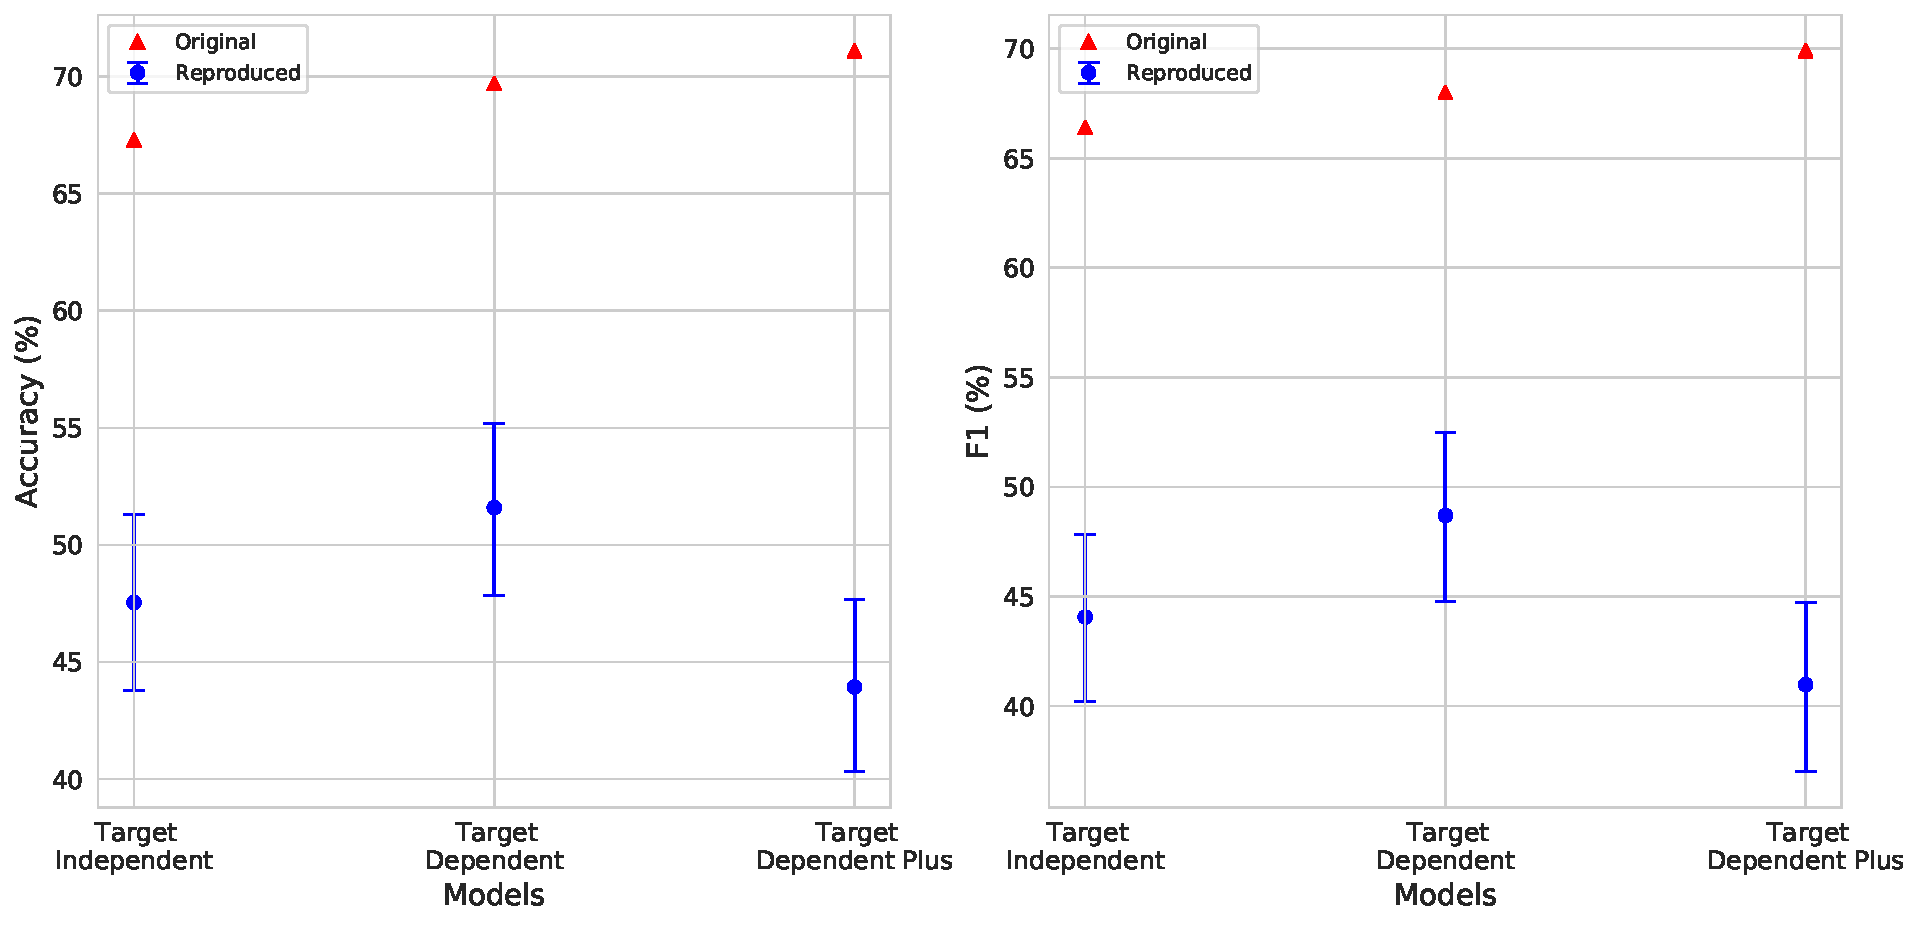
\includegraphics[scale=0.37]{images/reproducibility/vo/Target_Non_Scaled_Reproduction_Dong.pdf}
    \caption{Confidence intervals for the two tailed test for the reproduced models of \citet{vo2015target} using no scaling, on both the accuracy and macro F1 metrics. This was evaluated on the test set of \citet{dong-etal-2014-adaptive}.}
    \label{fig:repro_vo_Target_Non_Scaled_Reproduction_Dong}
\end{figure}

\subsection{Neural Pooling with Dependency Parsing}
%[I actually think he has more than that as they look at the break down of distinct sentiment. Not sure how I am going to get that metric in the theme of the thesis as this was the only paper that actually looked at the TDSA through that metric but it is a very good metric to use I think for TDSA]
To test if \citet{wang-etal-2017-tdparse} methods are reproducible, table 2 and 3 from their paper will be reproduced. These tables test their methods across two Twitter datasets, \citet{dong-etal-2014-adaptive} and their own Election Twitter dataset. To be comparable the SVM C-value is tuned using five-fold cross validation on the training data, as unlike \citet{vo2015target}, \citet{wang-etal-2017-tdparse} does not report what C-value they found to be optimal\footnote{The range of C-values \citet{wang-etal-2017-tdparse} used for tuning was not reported within the paper. However later on after the experiments within the thesis the C-value range used by \citet{wang-etal-2017-tdparse} was found through a function in their codebase: \url{https://github.com/bluemonk482/tdparse/blob/master/src/liblinear.py\#L91}.}. The range of C-values used within the tuning process is described within equation \ref{eq:repro_wang_c_values}, which is based on the exponential range suggested by \citet{hsu2003practical} with the addition of the default C-value ($1$) for linear SVMs in Scikit-learn \citep{pedregosa2011scikit}. The best found C-value for the accuracy metric, for each method, on each of the datasets can be seen in table \ref{table:repro_rep_wang_c}, these C-values will be used throughout unless otherwise stated. Additionally the same sentiment lexicons are used, but as stated earlier when using MinMax scaling the features are scaled between $0$ and $1$ rather than $-1$ and $1$. Also the same word vectors are used, which are the SSWE + w2v. As shown in figures \ref{fig:repro_wang_TDParse_Dong} and \ref{fig:repro_wang_TDParse_Election} the methods have been reproduced on both datasets.

\begin{equation}
    C=\{ 2^n | n = (i \times 2) - 17 ~for~0 < i < 10~and~i \in \Z \} \cup \{ 1 \} 
\label{eq:repro_wang_c_values}
\end{equation}

\FloatBarrier
\begin{table}[h!]
    \centering
    \begin{tabular}{|c|c|c|c|}
        \hline
         & \multicolumn{3}{c|}{Methods} \\
        \hline
        Dataset & TDParse Minus & TDParse & TDParse Plus \\
        \hline
        Dong & $2^{-5}$ & $2^{-7}$ & $2^{-7}$ \\
        \hline
        Election & $2^{-7}$ & $2^{-9}$ & $2^{-9}$ \\
        \hline
    \end{tabular}
    \caption{Best C-values for the accuracy metric for \citet{wang-etal-2017-tdparse} reproduced methods.}
    \label{table:repro_rep_wang_c}
\end{table}


\begin{figure}[!h]
    \centering
    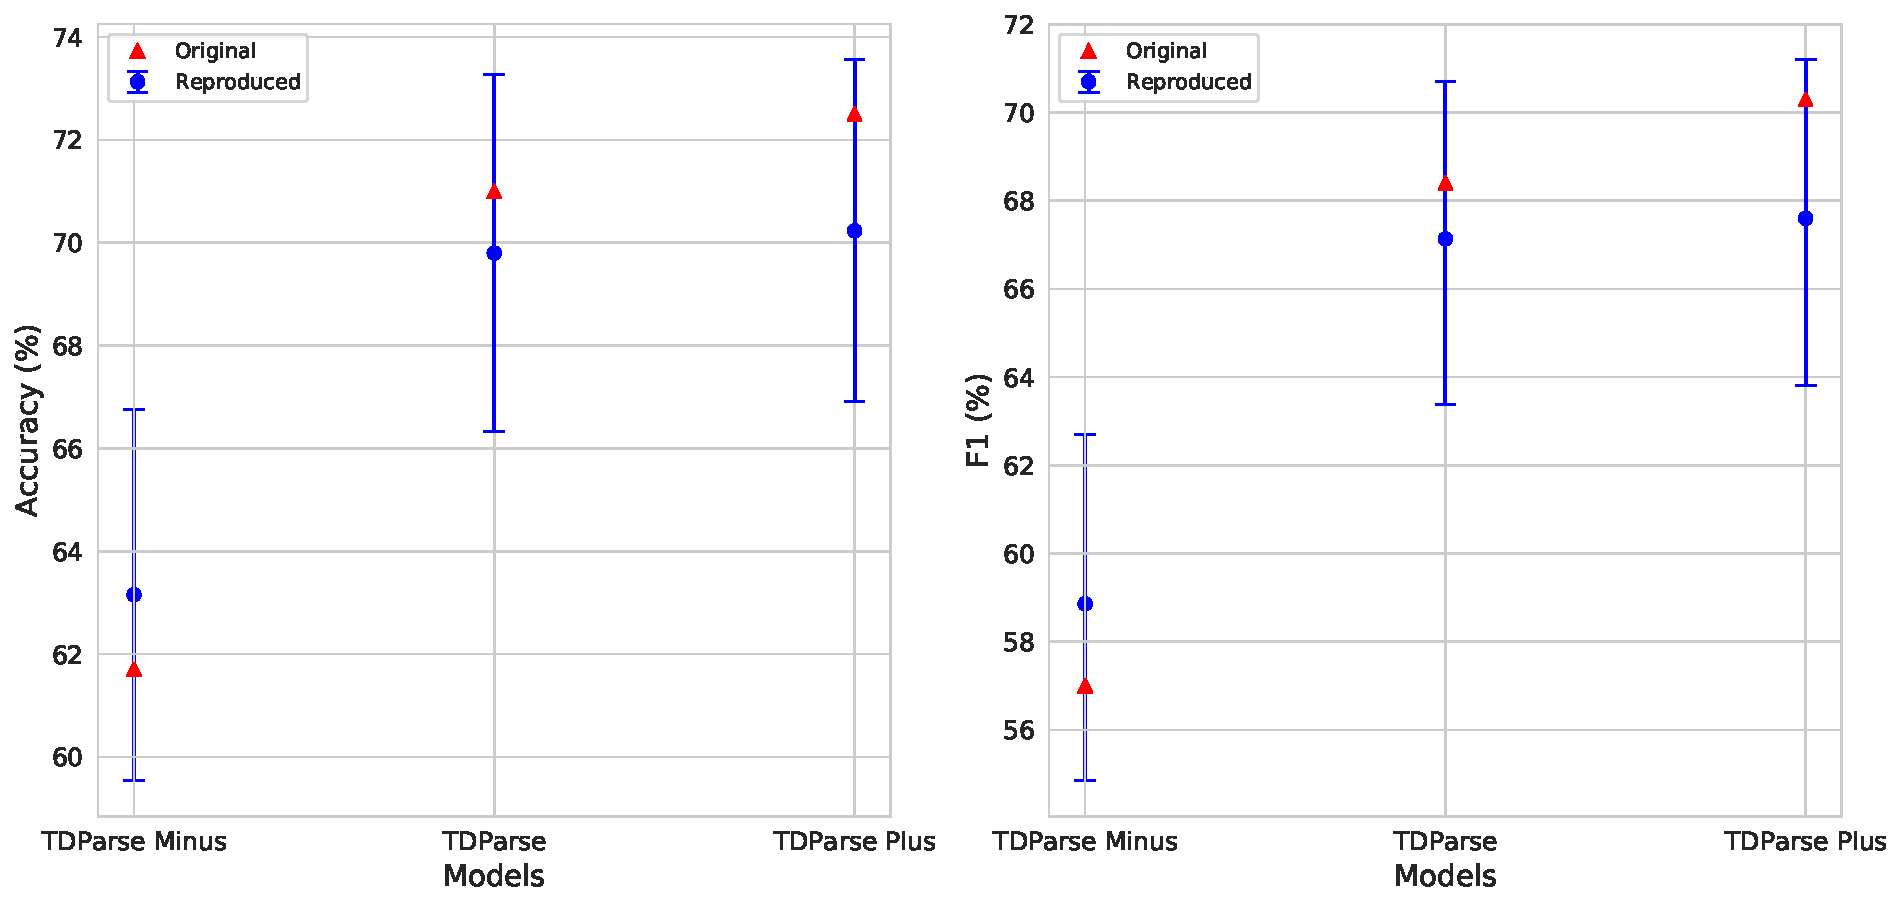
\includegraphics[scale=0.37]{images/reproducibility/wang/TDParse_Dong.pdf}
    \caption{Confidence intervals for the two tailed test on the \citet{dong-etal-2014-adaptive} test set, for the reproduced models of \citet{wang-etal-2017-tdparse}.}
    \label{fig:repro_wang_TDParse_Dong}
\end{figure}
\begin{figure}[!h]
    \centering
    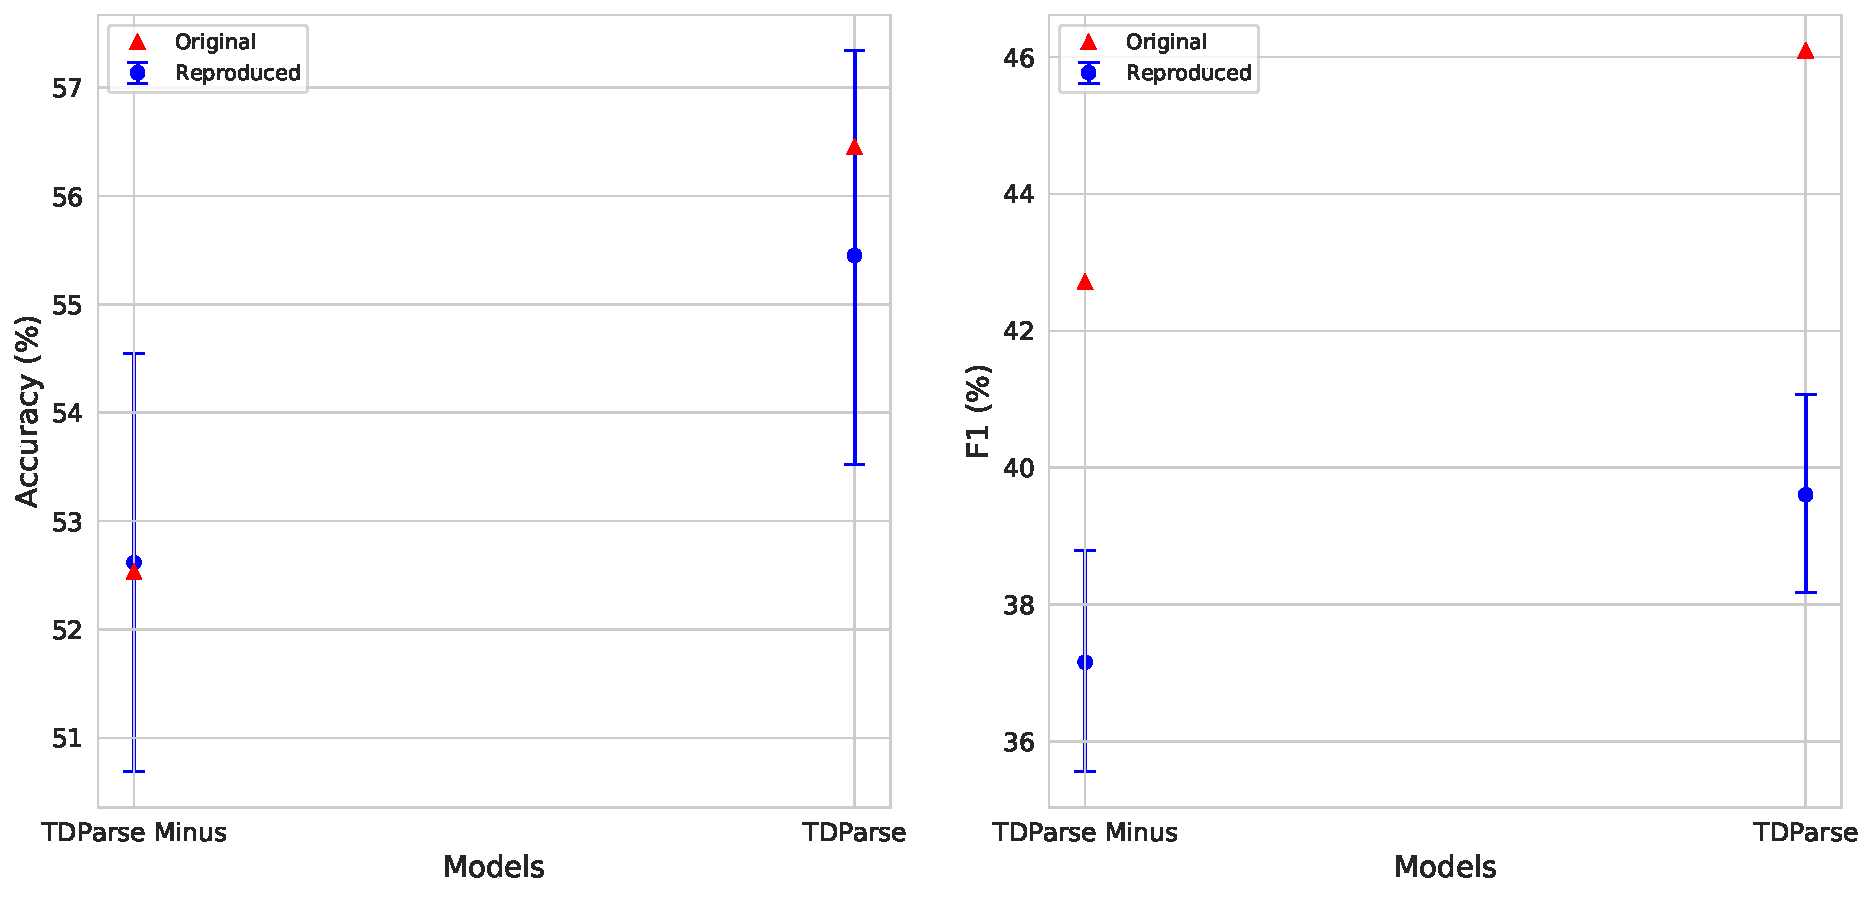
\includegraphics[scale=0.37]{images/reproducibility/wang/TDParse_Election.pdf}
    \caption{Confidence intervals for the two tailed test on the \citet{wang-etal-2017-tdparse} Election test set, for the reproduced models of \citet{wang-etal-2017-tdparse}.}
    \label{fig:repro_wang_TDParse_Election}
\end{figure}

 When using the MinMax scale range used by the original paper \citep{wang-etal-2017-tdparse} ($-1$ to $1$) the results are similar for all but the Election macro F1 scores, as shown in figures \ref{fig:repro_wang_TDParse_alt_scale_Dong} and \ref{fig:repro_wang_TDParse_alt_scale_Election}. However both the MinMax scale range used in this thesis, and the range used by \citet{wang-etal-2017-tdparse} create significantly different results to those of the original paper for the macro F1 metric on the Election dataset. Thus the same experiment is conducted, but using the C-values optimised for the macro F1 metric, where these values can be seen in table \ref{table:repro_rep_wang_c_macro_f1}\footnote{These C-values were tuned using the GloVe embeddings rather than SSWE + w2v. These embeddings were used because the C-values came from the data generated when performing the large scale C-value experiment that is performed later in this section.}. The results from this experiment can be seen in figures \ref{fig:repro_wang_TDParse_Election_macro_f1_c_values} and \ref{fig:repro_wang_TDParse_Election_alt_scaling_macro_f1_c_values} for the Election dataset\footnote{The results for the Dong dataset can be seen in appendix \ref{appendix_reproducibility_images} figures \ref{fig:repro_wang_TDParse_Dong_macro_f1_c_values} and \ref{fig:repro_wang_TDParse_Dong_alt_scaling_macro_f1_c_values}.} using the scaling range in this thesis and the scaling range of \citet{wang-etal-2017-tdparse} respectively. In both cases the macro F1 scores have increased and when using \citet{wang-etal-2017-tdparse} scaling range the original scores for macro F1 can be reproduced. Thus showing that within the original paper it is likely that they trained the methods separately with different C-values to optimise the different metric scores.  
 
 \FloatBarrier
 \begin{figure}[!h]
    \centering
    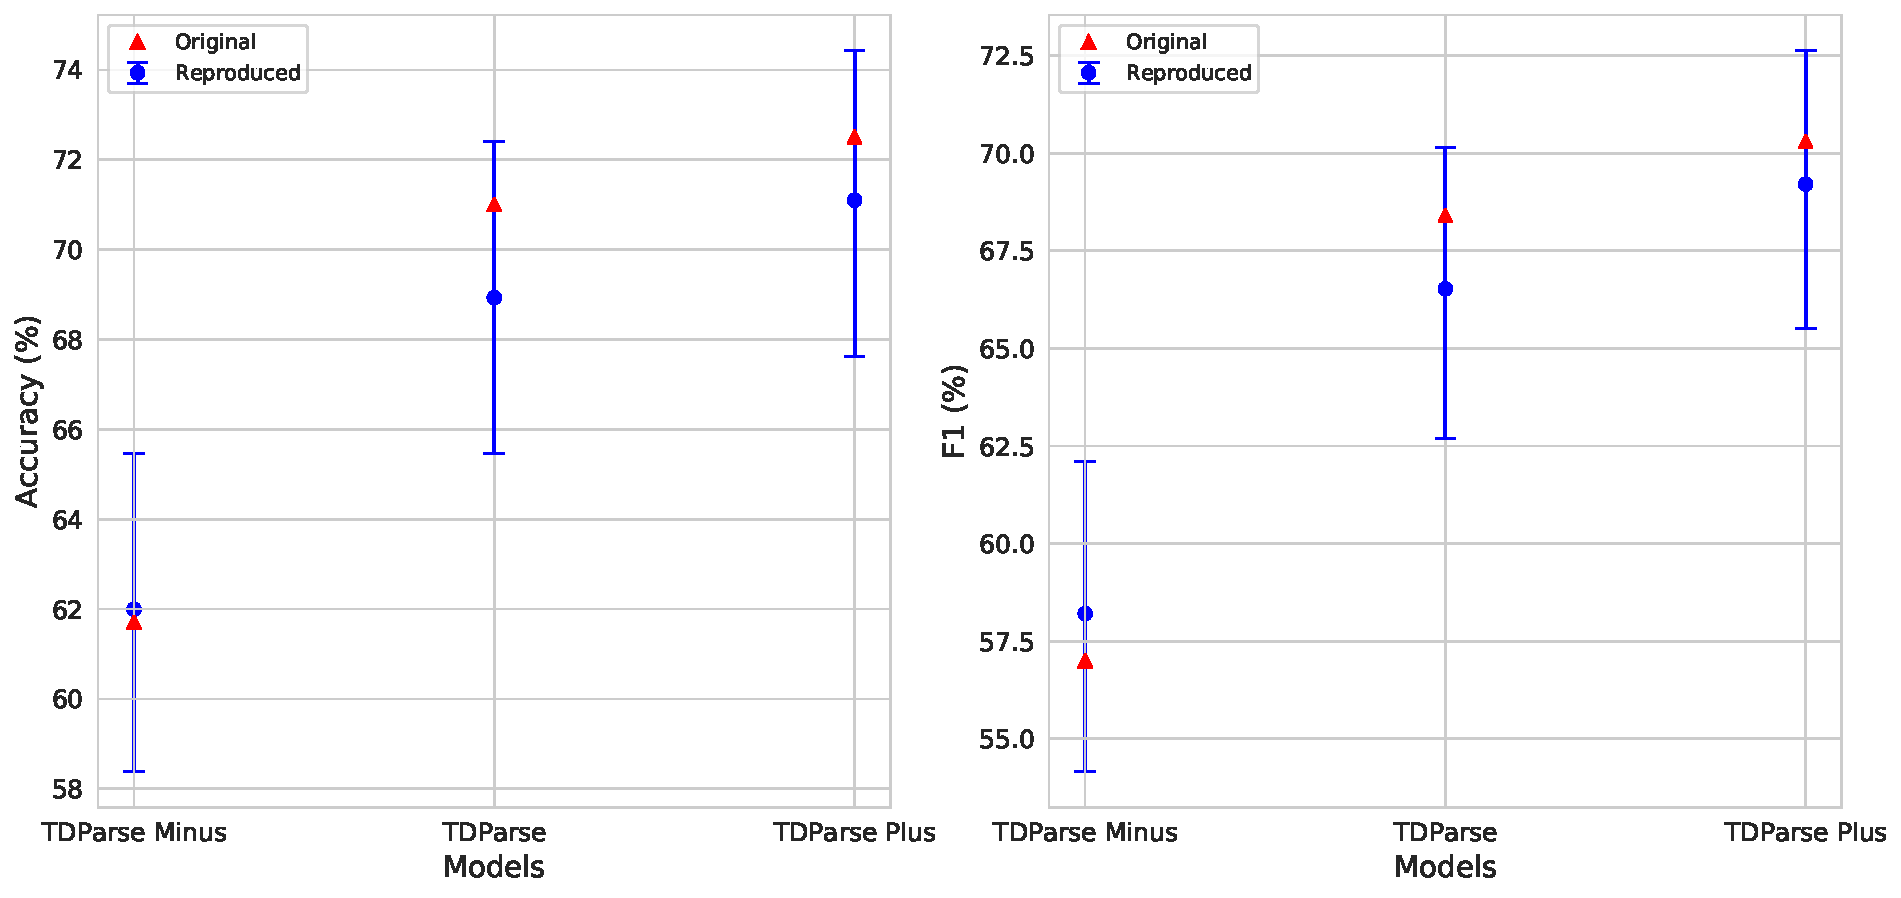
\includegraphics[scale=0.37]{images/reproducibility/wang/TDParse_alt_scale_Dong.pdf}
    \caption{Using the original MinMax scaling range of \citet{wang-etal-2017-tdparse}, the confidence intervals for the two tailed test on the \citet{dong-etal-2014-adaptive} test set.}
    \label{fig:repro_wang_TDParse_alt_scale_Dong}
\end{figure}
\begin{figure}[!h]
    \centering
    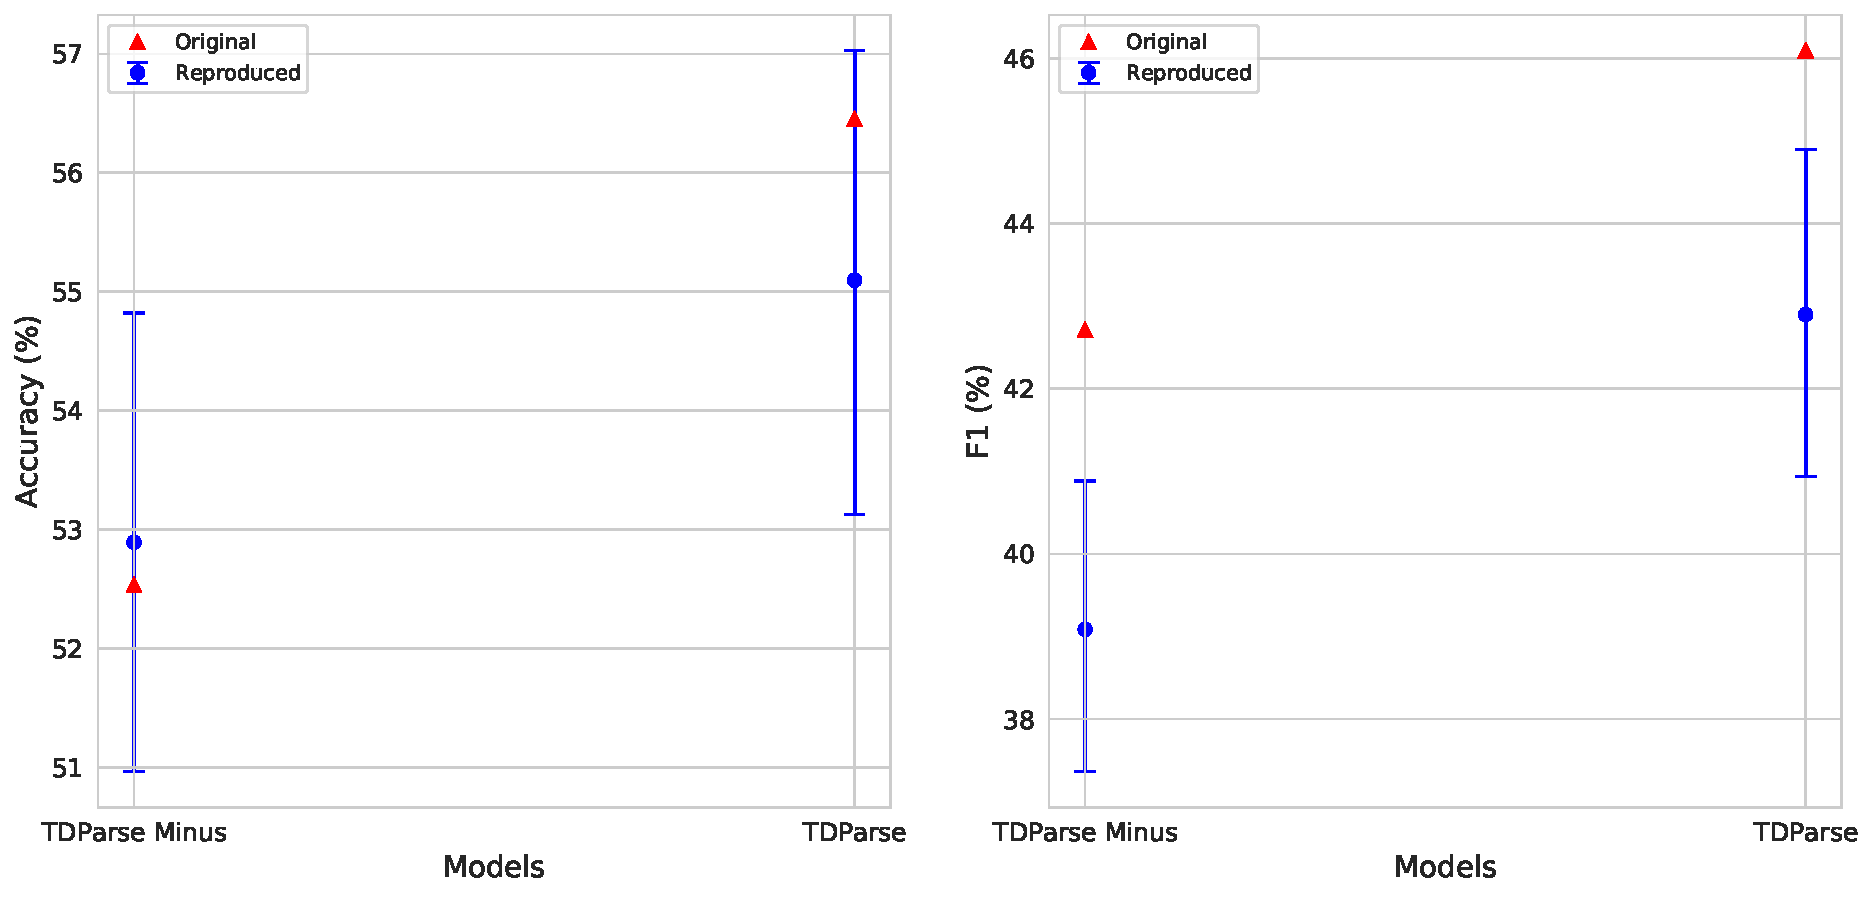
\includegraphics[scale=0.37]{images/reproducibility/wang/TDParse_alt_scale_Election.pdf}
    \caption{Using the original MinMax scaling range of \citet{wang-etal-2017-tdparse}, the confidence intervals for the two tailed test on the \citet{wang-etal-2017-tdparse} Election test set.}
    \label{fig:repro_wang_TDParse_alt_scale_Election}
\end{figure}

\begin{table}[h!]
    \centering
    \begin{tabular}{|c|c|c|c|}
        \hline
         & \multicolumn{3}{c|}{Methods} \\
        \hline
        Dataset & TDParse Minus & TDParse & TDParse Plus \\
        \hline
        Election & $2^{-3}$ & $2^{-7}$ & $2^{-7}$ \\
        \hline
    \end{tabular}
    \caption{Best C-values for the macro F1 metric for \citet{wang-etal-2017-tdparse} reproduced methods.}
    \label{table:repro_rep_wang_c_macro_f1}
\end{table}


\begin{figure}[!h]
    \centering
    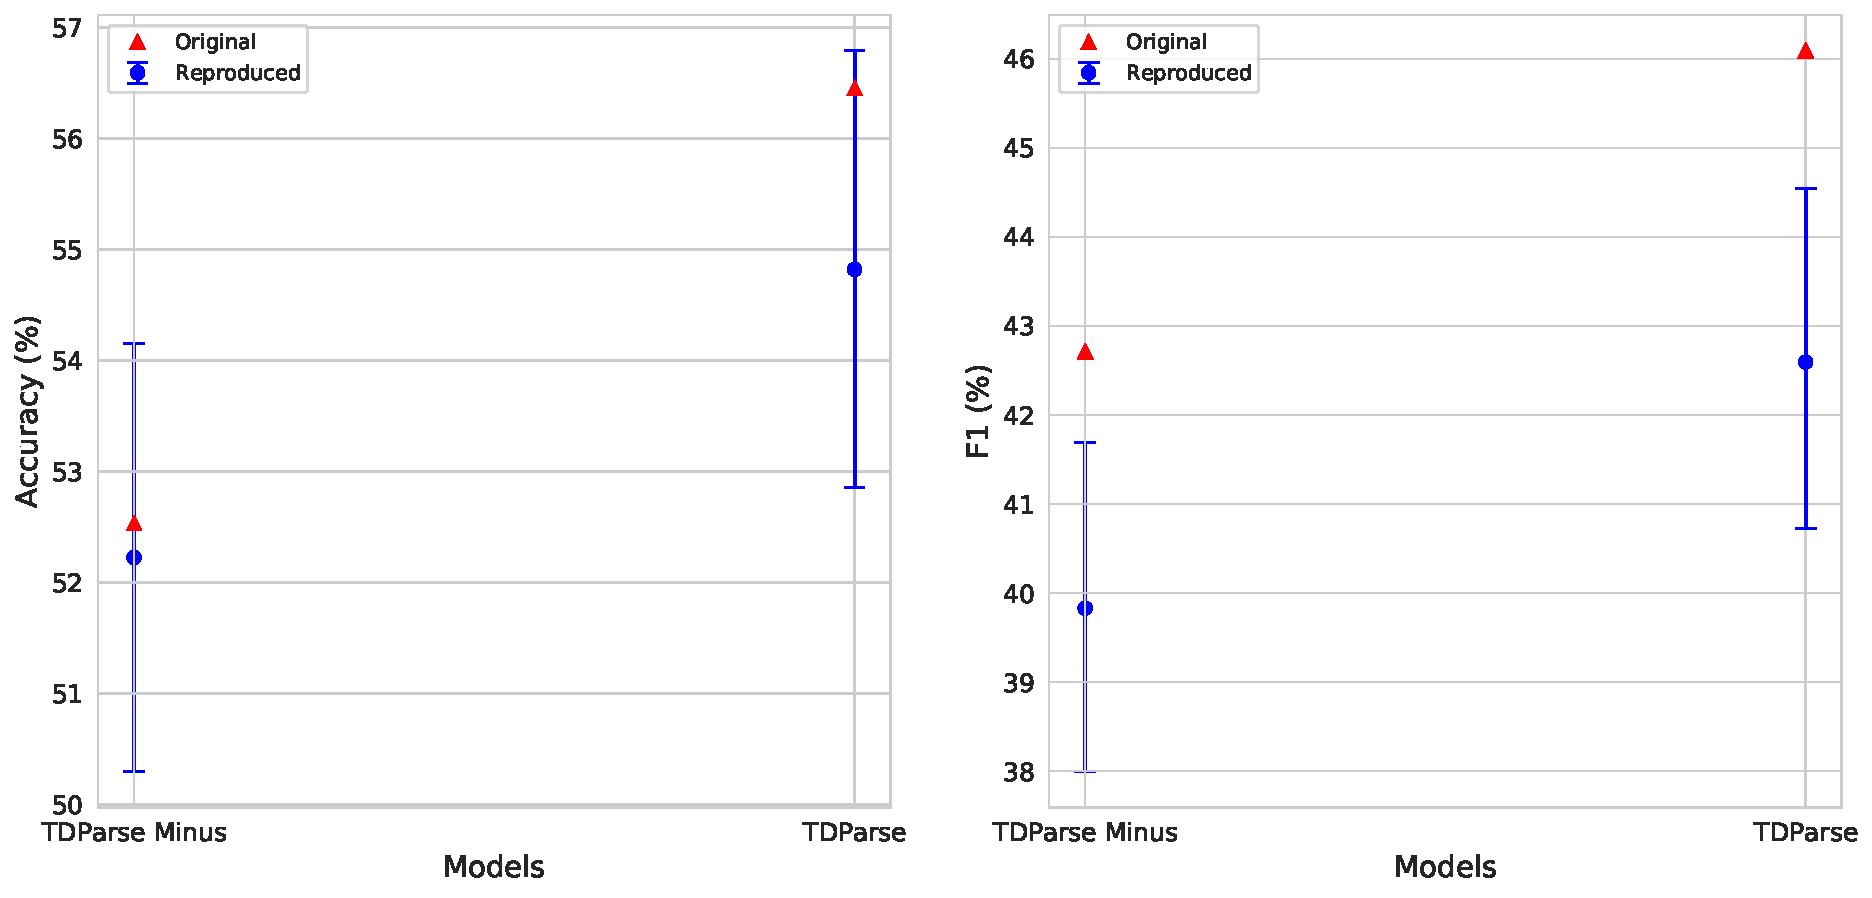
\includegraphics[scale=0.37]{images/reproducibility/wang/TDParse_F1_C_value_Election.pdf}
    \caption{Using the C-values optimised for macro F1 metric, the confidence intervals for the two tailed test on the \citet{wang-etal-2017-tdparse} Election test set.}
    \label{fig:repro_wang_TDParse_Election_macro_f1_c_values}
\end{figure}

\begin{figure}[!h]
    \centering
    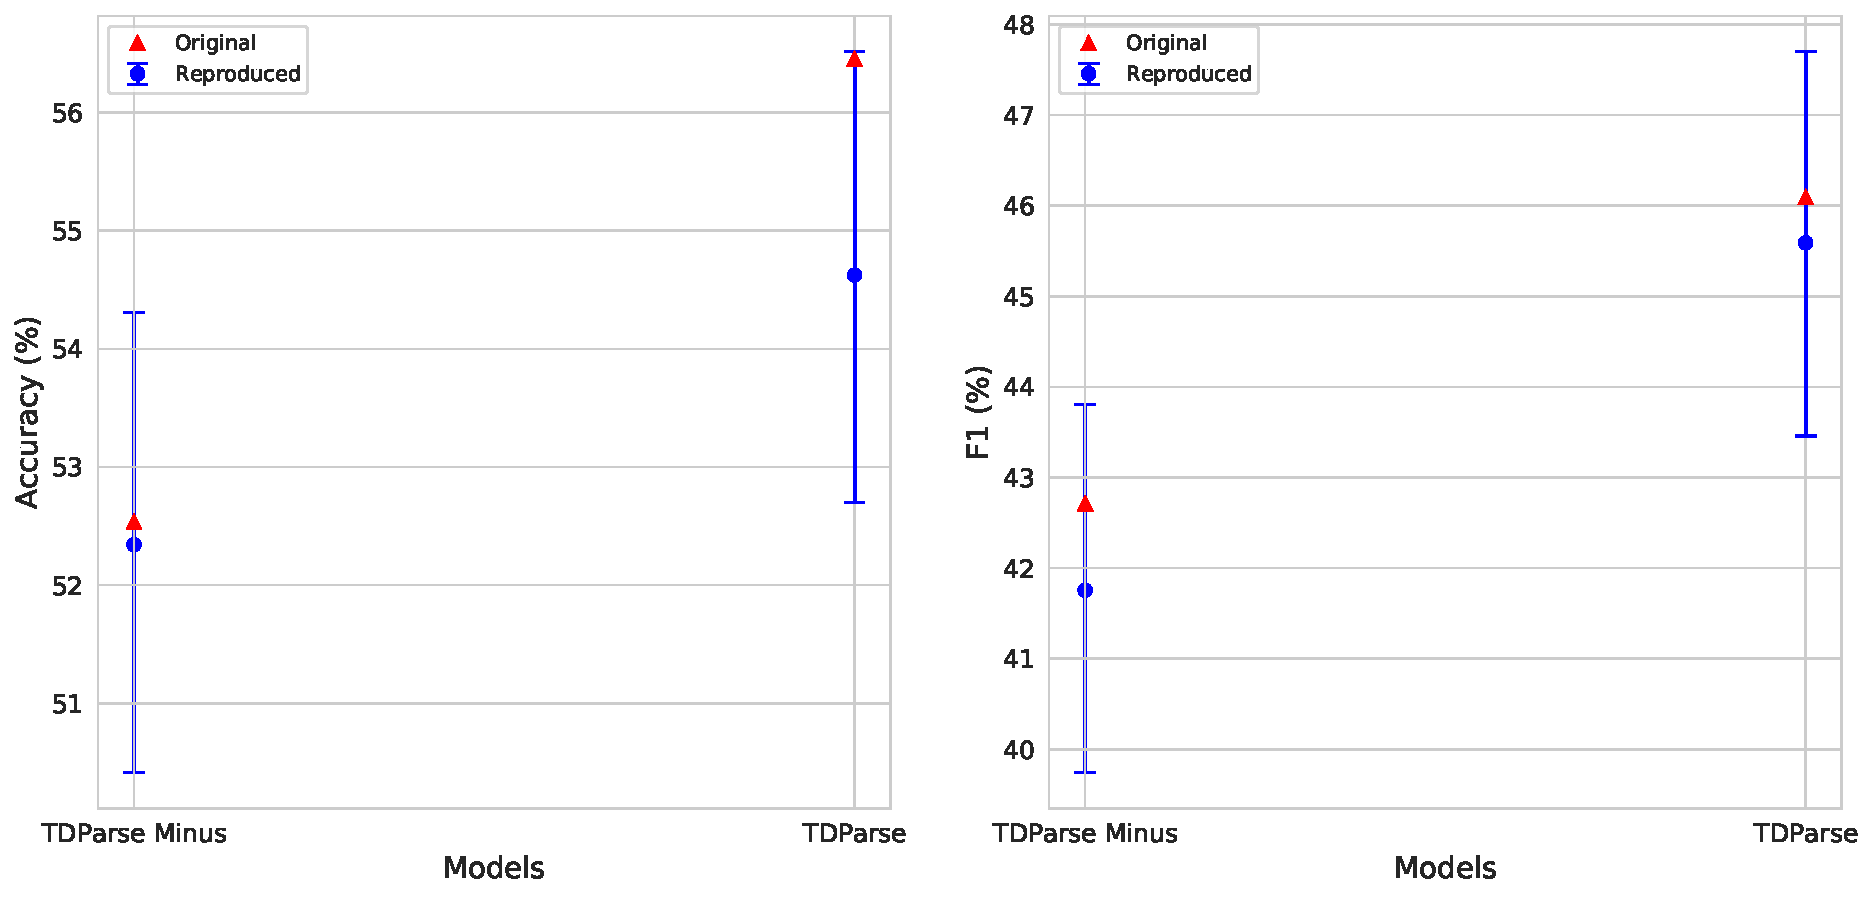
\includegraphics[scale=0.37]{images/reproducibility/wang/TDParse_F1_C_value_alt_scale_Election.pdf}
    \caption{Using the C-values optimised for macro F1 metric with the original MinMax scaling range of \citet{wang-etal-2017-tdparse}, the confidence intervals for the two tailed test on the \citet{wang-etal-2017-tdparse} Election test set.}
    \label{fig:repro_wang_TDParse_Election_alt_scaling_macro_f1_c_values}
\end{figure}

As scaling is not mentioned in the paper and only stated within the run command of the codebase, the same experiment is repeated with methods that do not scale the features. As shown in figures \ref{fig:repro_wang_TDParse_Dong_no_scale} and \ref{fig:repro_wang_TDParse_Election_no_scale} all results are significantly different and in most cases do not preserve rank order. Thus showing here again the high importance of scaling.

\begin{figure}[!h]
    \centering
    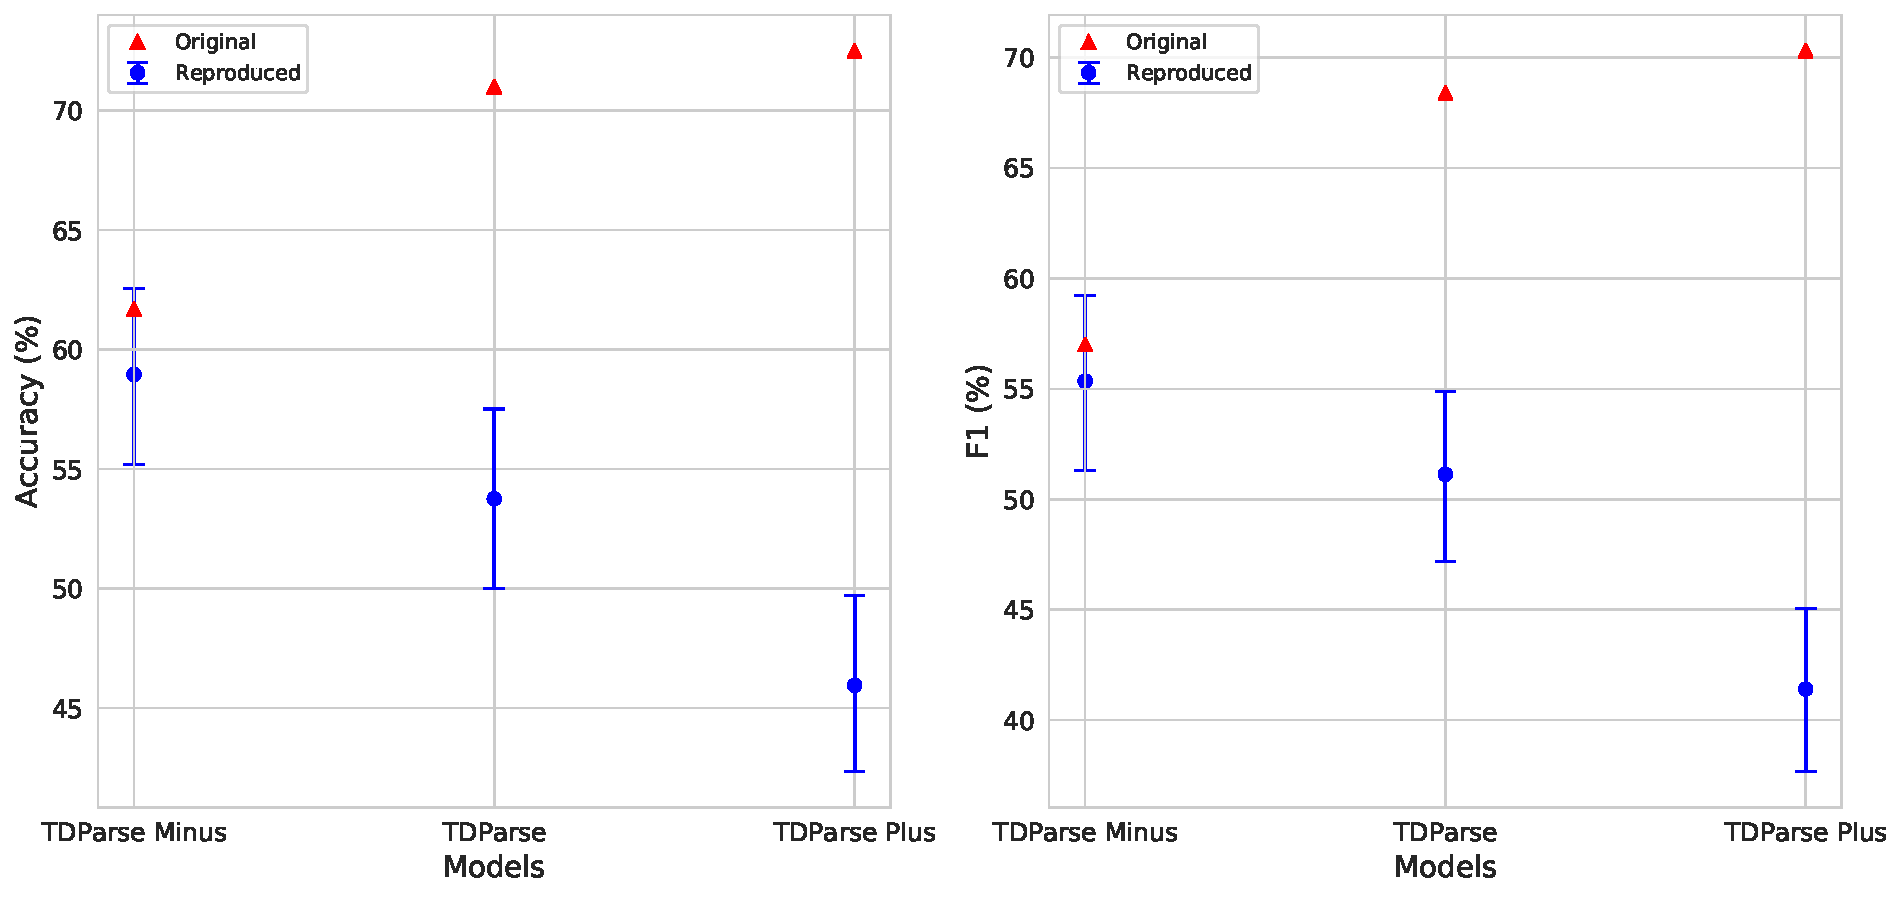
\includegraphics[scale=0.37]{images/reproducibility/wang/TDParse_no_scale_Dong.pdf}
    \caption{Using no scaling, the confidence intervals for the two tailed test on the \citet{dong-etal-2014-adaptive} test set.}
    \label{fig:repro_wang_TDParse_Dong_no_scale}
\end{figure}
\begin{figure}[!h]
    \centering
    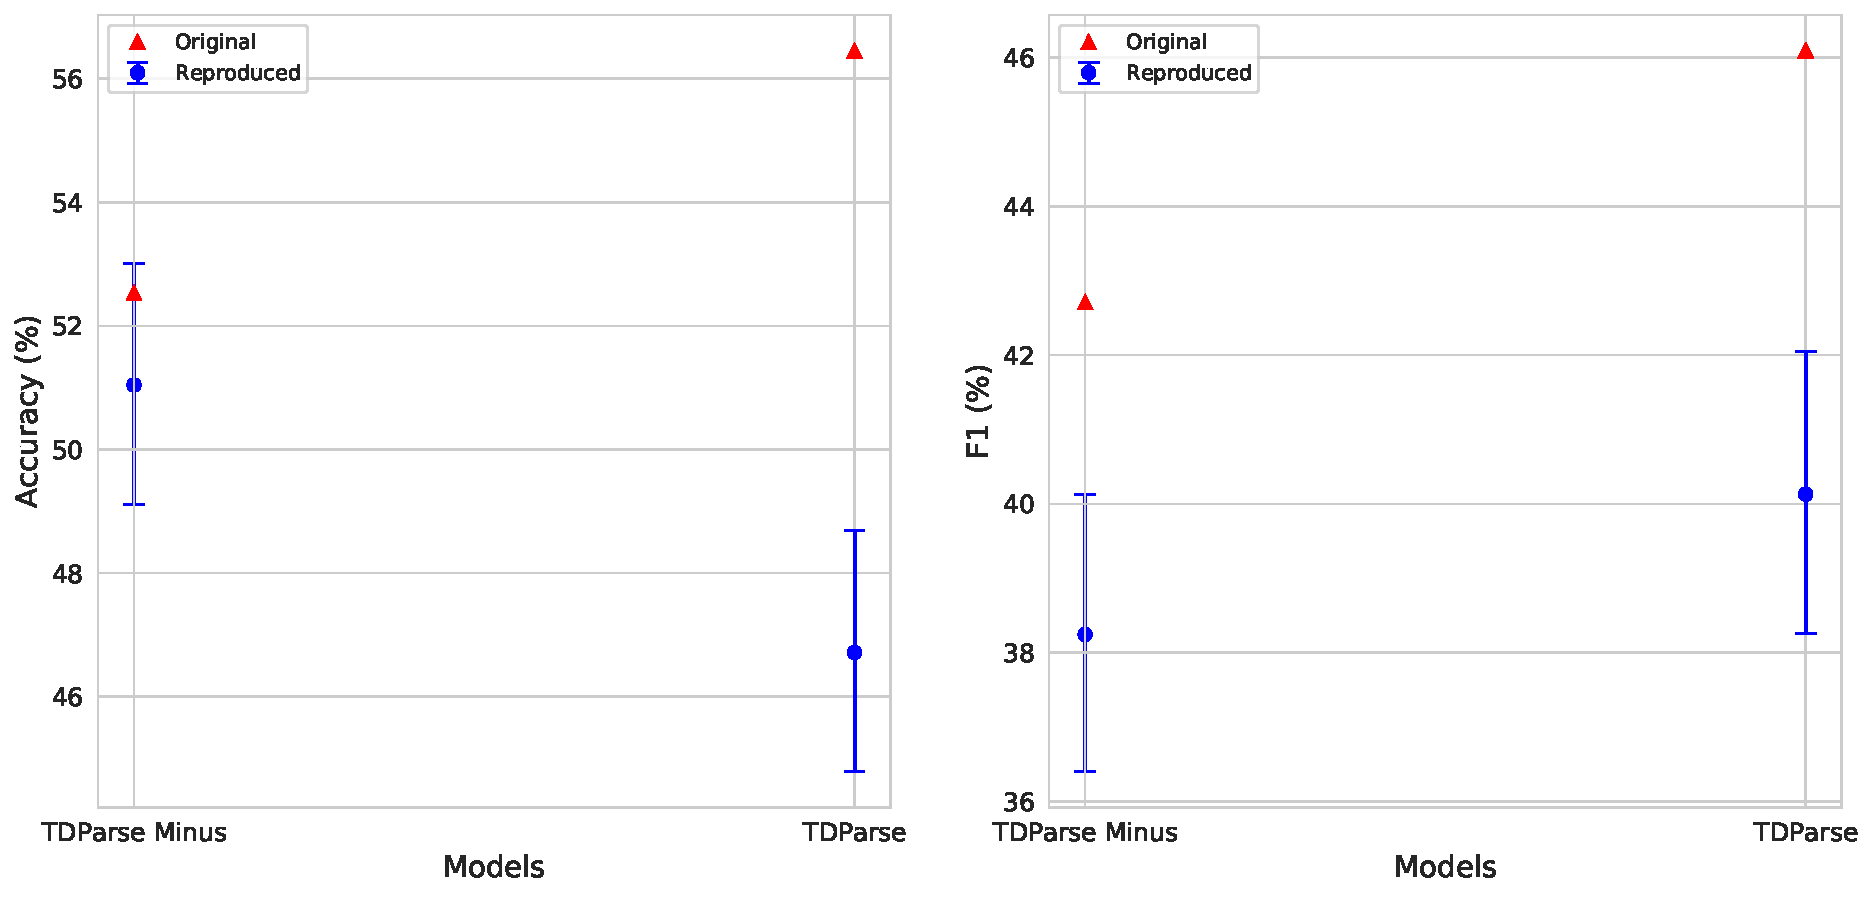
\includegraphics[scale=0.37]{images/reproducibility/wang/TDParse_no_scale_Election.pdf}
    \caption{Using no scaling, the confidence intervals for the two tailed test on the \citet{wang-etal-2017-tdparse} Election test set.}
    \label{fig:repro_wang_TDParse_Election_no_scale}
\end{figure}

The last two sets of experiments explores the importance of the C-value within the SVM that is used in the NP methods and scaling. As it has been shown that the C-value is statistically significantly important to recreate the macro F1 score within the Election dataset experiments for \citet{wang-etal-2017-tdparse} and for all NP methods scaling is statistically significant. These sets of experiments will explore how significant these two parameters are within the NP methods, whereby all of the NP methods from \citet{vo2015target} and \citet{wang-etal-2017-tdparse} will be used to make the findings more robust. Furthermore to make the findings generalisable the methods will be applied to all six datasets from table \ref{table:repro_dataset_stats}. The experiments will use five-fold cross validation on the training sets to ensure the test set is not used, and thus allow researches to use these findings without overfitting to the test sets. In all experiments the mean best performing configuration of the method for either the accuracy or macro F1 metric will be compared against all other configurations using a one sided significant test. The number of folds that the mean best configuration is significantly better than the other configurations will be corrected using Bonferroni. 

As these experiments are conducted on various different datasets, the methods will use the general non-type and non-task specific GloVe embeddings that are also the most popular in the area. For sentiment lexicon based methods the same lexicons used by \citet{wang-etal-2017-tdparse} will be used as they are a superset of the lexicons used by \citet{vo2015target} and the lexicons come from various types of data\footnote{The lexicons used originate from MPQA \citep{wilson-etal-2005-recognizing} (news data), NRC \citep{mohammad-turney-2010-emotions} (general data chosen from a dictionary based on word frequency from Google n-gram corpus \citep{brantsweb}), and \citet{hu2004mining} (review data).}. The Stanford CoreNLP tokeniser \citep{manning-etal-2014-stanford} will be used in preference to the Twitter specific tokeniser; Twokenizer \citep{gimpel-etal-2011-part} to avoid type specific tools. For \citet{wang-etal-2017-tdparse} methods that require a dependency parser the TweeboParser \citep{kong-etal-2014-dependency} will be used on all datasets but the Laptop and Restaurant datasets, whereby the Stanford CoreNLP dependency parser will be used. This decision was made before realising the importance of a dependency parser creating multiple roots for \citet{wang-etal-2017-tdparse} methods and Stanford's parser does not create multiple roots. Thus in effect Stanford's parser will create a context that is almost identical to the whole text context\footnote{The reason it is not the same is due to the context not including the target word(s). Also Stanford's parser requires the text to go through their sentence splitter first, which in some cases does cause the text to be split up.}. Stanford's parser was chosen due to the Laptop and Restaurant datasets coming from a different type of data (review rather than social media) and thus is believed to require a more type relevant parser, such as the Stanford parser. 

The SVM C-value is part of the L2-regularised L2-loss function of the linear SVM which can be seen in equation \ref{eq:repro_svm} (taken from equation 1 in \citep{fan2008liblinear}). The L2-regularisation in the equation is $\frac{1}{2}w^Tw$ and the rest is the L2-loss. As can be seen the C-value determines the amount of weight the L2-loss has on the overall loss function. Thus if the C-value is large the effect of the regularisation is small, which would more likely cause the model to overfit to the training data.

\begin{equation}
    \frac{1}{2}w^{T}w + C\sum_{i=1}^{l}(\max(0, 1 - y_{i}w^{T}x_i))^2
    \label{eq:repro_svm}
\end{equation}

The C-values that will be tested here are the same as those evaluated for the reproduction of \citet{wang-etal-2017-tdparse}, shown in equation \ref{eq:repro_wang_c_values}. Figures \ref{fig:repro_parameters_c_values_accuracy} and \ref{fig:repro_parameters_c_values_macro_f1} show the mean best C-values for each method on each dataset for the accuracy and macro F1 metric respectively. In both cases it can be seen that all methods are significantly sensitive to the choice in C-value no matter the dataset. In most cases and more so for the accuracy metric the default C-value from scikit-learn \citep{pedregosa2011scikit} ($1$) is significantly worse than the mean best. It would be assumed that datasets that are small like YouTuBean would prefer a small C-value to stop the methods from overfitting, but that does not seem to be the case. Rather it would appear that for both the accuracy and macro F1 score each have their own preferable band of C-values. For accuracy, generally $7.81e^{-3}$ performs well on all methods and datasets, whereas for macro F1 it is dataset and method specific. Furthermore a C-value that performs best for accuracy could be significantly worse than the best C-value for macro F1, of which this happens the most on the Election dataset. For the mean best scores produced by these C-values for all methods on all datasets see figures \ref{fig:repro_parameters_c_accuracy_plot} and \ref{fig:repro_parameters_c_macro_f1_plot} in appendix \ref{appendix_reproducibility_images}.

\begin{figure}[!h]
    \centering
    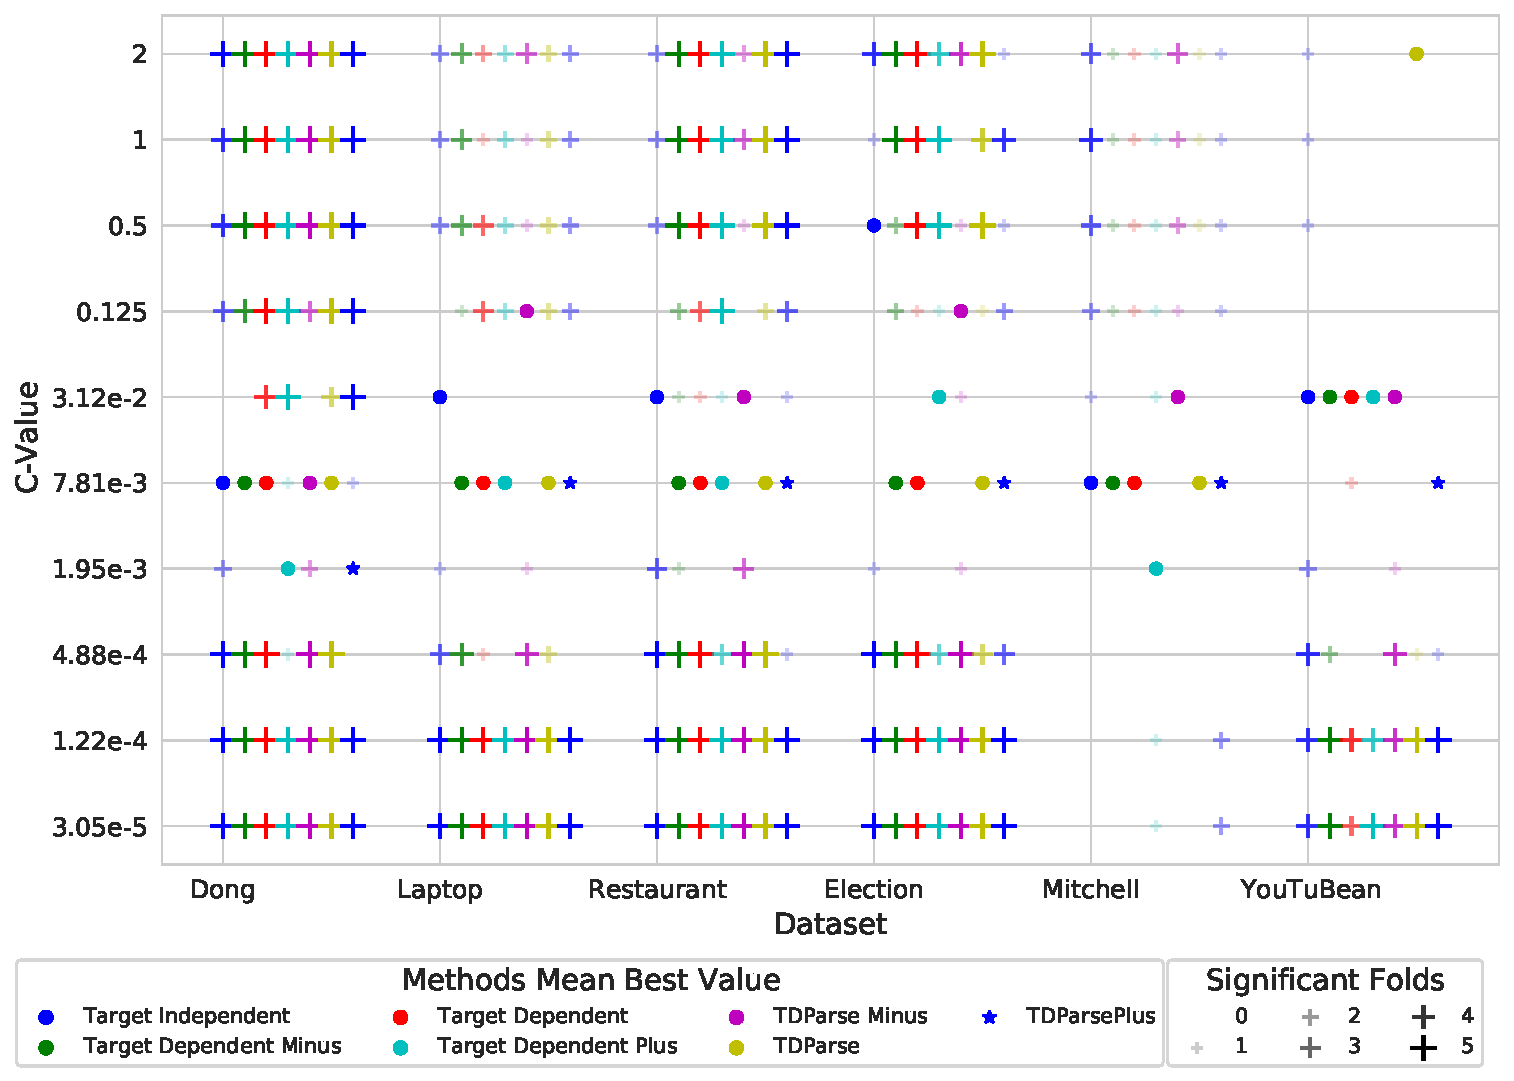
\includegraphics[scale=0.47]{images/reproducibility/Parameters/C_Value/C_Sig_Plot_Accuracy.pdf}
    \caption{For the accuracy metric the mean best C-value for each method and dataset represented by dots and star. The size of the cross indicates the number of folds the mean best C-value is significantly better than the other C-values for the given method and dataset.}
    \label{fig:repro_parameters_c_values_accuracy}
\end{figure}
\begin{figure}[!h]
    \centering
    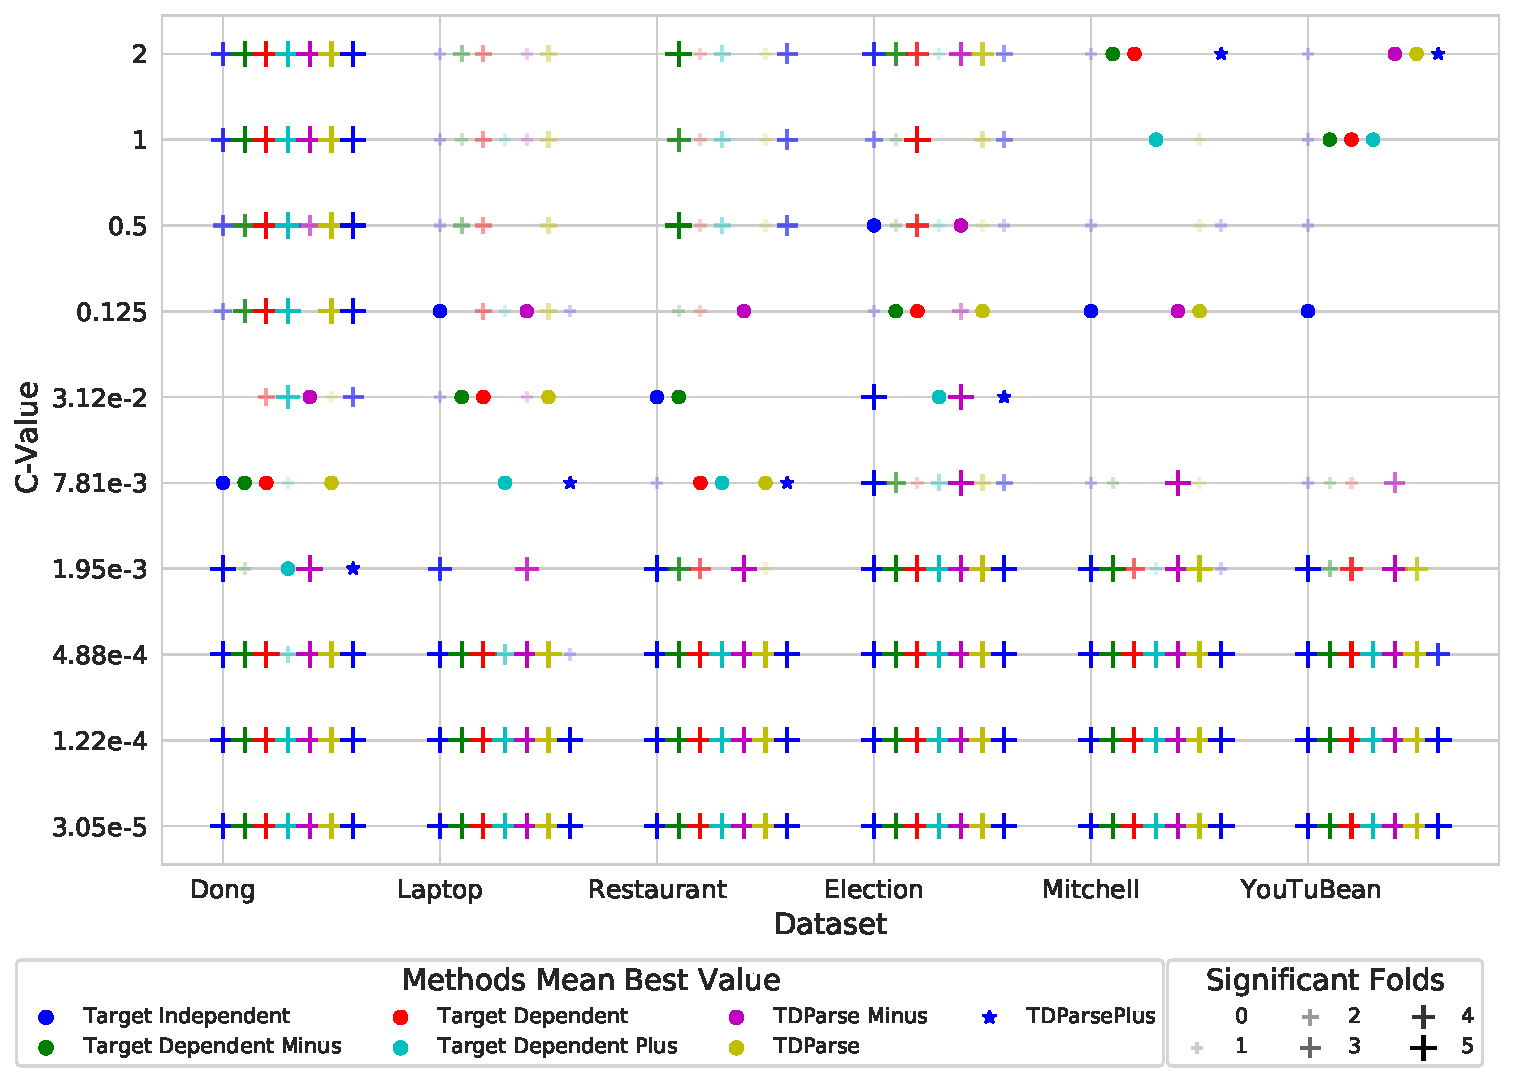
\includegraphics[scale=0.47]{images/reproducibility/Parameters/C_Value/C_Sig_Plot_F1.pdf}
    \caption{For the macro F1 metric the mean best C-value for each method and dataset represented by dots and star. The size of the cross indicates the number of folds the mean best C-value is significantly better than the other C-values for the given method and dataset.}
    \label{fig:repro_parameters_c_values_macro_f1}
\end{figure}
\clearpage

MinMax scaling with the scale range of $0$ to $1$, rather than \citet{wang-etal-2017-tdparse} $-1$ to $1$, will be compared to not scaling. When performing these experiments the optimal C-value for each method on each dataset for the accuracy metric is used, which was found from the last experiment. The results can be seen in figures \ref{fig:repro_parameters_c_values_accuracy} and \ref{fig:repro_parameters_c_values_macro_f1}. It can be clearly seen in all cases for the accuracy metric and the majority for the macro F1 metric that scaling is statistically significant no matter the method nor dataset, with the caveat of Mitchell for the macro F1 metric. For the mean best scores produced by these scaling experiments for all methods on all datasets see figures \ref{fig:repro_parameters_scaling_accuracy_plot} and \ref{fig:repro_parameters_scaling_macro_f1_plot} in appendix \ref{appendix_reproducibility_images}.

\begin{figure}[!h]
    \centering
    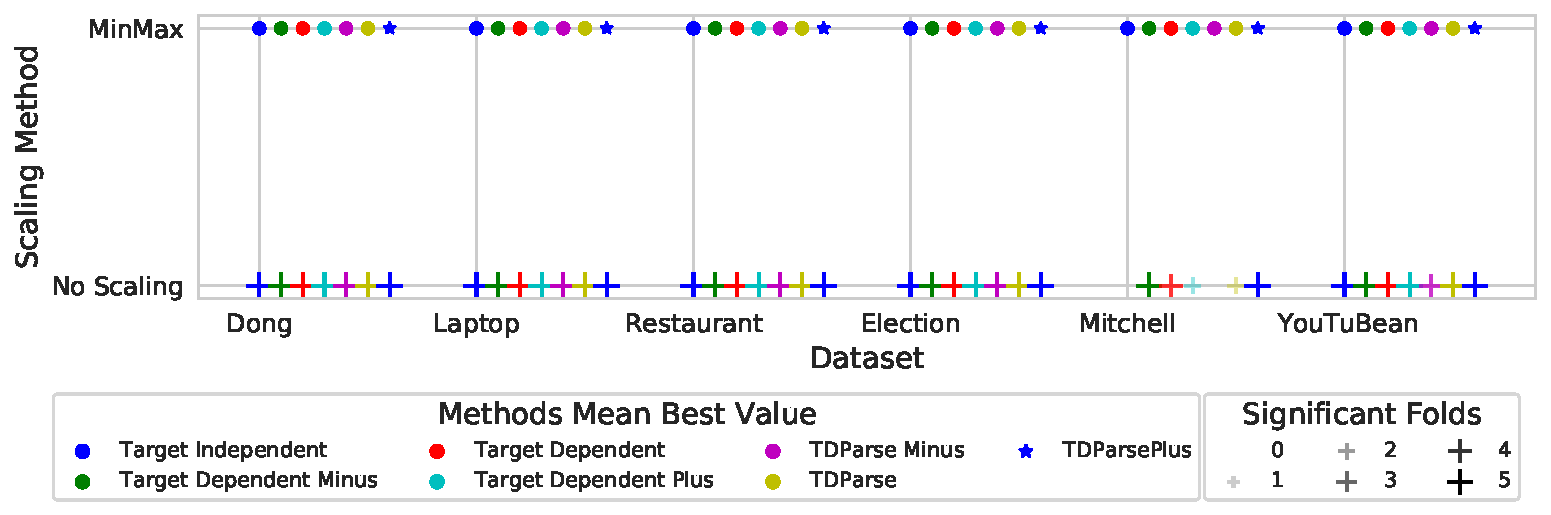
\includegraphics[scale=0.47]{images/reproducibility/Parameters/Scaling/Scaling_Sig_Plot_Accuracy.pdf}
    \caption{For the accuracy metric the mean best scaling method for each method and dataset represented by dots and star. The size of the cross indicates the number of folds the mean best scaling method is significantly better than the other scaling method for the given method and dataset.}
    \label{fig:repro_parameters_scaling_accuracy}
\end{figure}
\begin{figure}[!h]
    \centering
    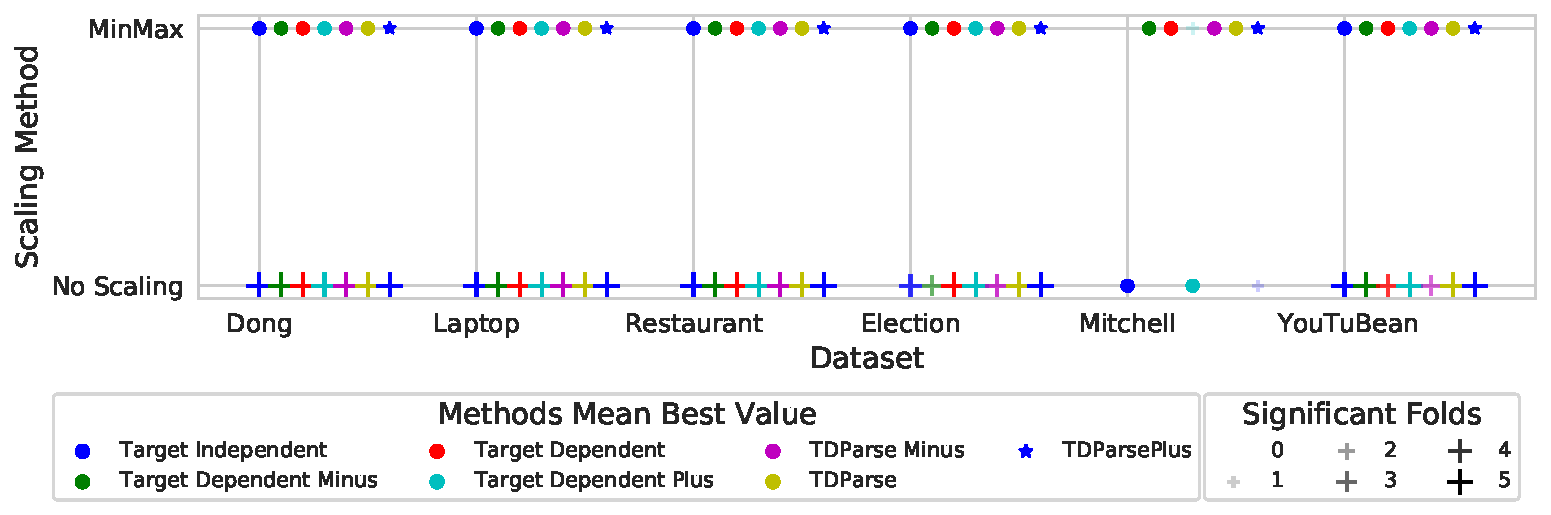
\includegraphics[scale=0.47]{images/reproducibility/Parameters/Scaling/Scaling_Sig_Plot_F1.pdf}
    \caption{For the macro F1 metric the mean best scaling method for each method and dataset represented by dots and star. The size of the cross indicates the number of folds the mean best scaling method is significantly better than the other scaling method for the given method and dataset.}
    \label{fig:repro_parameters_scaling_macro_f1}
\end{figure}


% Furthermore \citet{reimers-gurevych-2017-reporting} found that the same NN based sequence labelling method can produce statistically significantly different results based on the random seed the method was initialised with.

\subsection{LSTM}
\label{section:repro_lstm}

It has been found that in the previous work it is difficult to either reproduce \citep{tay2018learning} or replicate \citep{chen-etal-2017-recurrent} \citet{tang-etal-2016-effective} LSTM based methods, most specifically the TDLSTM version, as shown by table \ref{table:repro_tang_authors_differences}\footnote{The original \citet{tang-etal-2016-effective} methods as stated in this section were never originally evaluated on the Laptop or Restaurant datasets. However the original authors within another paper \citep{tang-etal-2016-aspect} evaluated the TDLSTM method they created on the Laptop and Restaurant datasets and that is what is meant by original authors within the table.}. Based on these findings the methods in \citet{tang-etal-2016-effective} are reproduced. The reproduced methods are evaluated on \citet{dong-etal-2014-adaptive} Twitter dataset and use the same GloVe Twitter 100 dimension embeddings \citep{pennington-etal-2014-glove}. All methods used Stochastic Gradient Descent (SGD) with a learning rate of $0.01$, a cross entropy loss, and the hidden dimension of all LSTMs equal to the dimension of the embedding being used. However the paper did not state the number of epochs the method was trained for thus early stopping is used keeping track of the loss value with a patience of $10$. As early stopping requires a validation set, the training set is split $80\%$ training and $20\%$ validation. The paper also mentioned that they ``set the clipping threshold of softmax layer as 200'' \citep{tang-etal-2016-effective} as this did not make sense, this was not used. Lastly all weights were initialised using $\mathcal{U}(-\sqrt{k}, \sqrt{k})$\footnote{This is the default initialisation within PyTorch \citep{NEURIPS2019_9015} and AllenNLP \citep{gardner-etal-2018-allennlp}.} where $k = \frac{1}{\text{embedding dimension}}$. The original initialisation from \citet{tang-etal-2016-effective}, $\mathcal{U}(-0.003, 0.003)$, always overfitted to the dominant class\footnote{Which is neutral for \citet{dong-etal-2014-adaptive} as shown by table \ref{table:repro_dataset_sent_dist}.} when used in the reproduced methods, hence the difference in the initialisation distributions. The tokeniser used was Spacy, as the original tokeniser that was used was not stated in the paper\footnote{To note in the original paper \citep{moore-rayson-2018-bringing} that this chapter is based on the results for \citet{tang-etal-2016-effective} did use the original weight initialisation of \citet{tang-etal-2016-effective} ($\mathcal{U}(-0.003, 0.003)$) and could still reproduce the results. The main implementation difference between \citet{moore-rayson-2018-bringing} and this chapter is that here PyTorch \citep{NEURIPS2019_9015} and AllenNLP \citep{gardner-etal-2018-allennlp} is used rather than Keras \citep{chollet2015keras} and also the Spacy tokeniser is used rather than Twokenizer \cite{gimpel-etal-2011-part} tokeniser. It is unknown why the original weight initialisation did not work within the code implementation of this chapter, it is believed it could be due to subtle differences between Keras and PyTorch.}. 




\begin{table}[!h]
    \centering
    \begin{tabular}{|c|c|c|}
        \hline
        Authors & Restaurant & Laptop\\
        \hline
        \posbox{\citet{tang-etal-2016-aspect}} & 75.63 & 68.13 \\
        \hline
        \negbox{\citet{chen-etal-2017-recurrent}} & 78.00 & 71.83 \\
        \hline
        \neubox{\citet{tay2018learning}} & 69.73 & 62.38 \\
        \hline
        \multicolumn{3}{|c|}{\centering \cbox{lightblue} Original authors \quad \cbox{lightred} Replicated \quad \cbox{lightgrey} Reproduced} \\
        \hline
    \end{tabular}
    \caption{Accuracy of the TDLSTM method by the different authors on the Restaurant and Laptop datasets.}
    \label{table:repro_tang_authors_differences}
\end{table}

The results from the experiment can be seen in table \ref{table:tang_twitter_100_results} and figure \ref{fig:repro_tang_LSTM_DIST_ACC_F1} whereby each reproduced method has been ran $20$ times. Running each method $20$ times using different random seeds allows the methods to take into account the random initialisation problem \citep{reimers-gurevych-2017-reporting}. It can be seen that if the maximum score is used the original and reproduced results are quite close, and statistically similar as shown by figure \ref{fig:repro_tang_LSTM_ACC_F1}\footnote{The best run for accuracy is not always the same best run for macro F1. Therefore we only use the best run for each method based on the metric being evaluated.}. Furthermore based on the maximum score the rank of the methods are the same as the original, thus the methods have been reproduced successfully. However the difference between the maximum result and the minimum can be quite large, especially for the macro F1 metric.

\begin{table}[!h]
    \centering
    \begin{tabular}{|c|c|c|c|c|c|}
\hline
Metric &    Method    &   Max &   Mean &   Min & Original \\
\hline
Accuracy & LSTM &  64.31 &  62.93 &  61.42 & 66.5 \\
& TDLSTM &  69.36 &  \textbf{67.23} &  \textbf{65.46} & 70.8 \\
& TCLSTM &  \textbf{70.23} &  66.74 &  64.74 & 71.5 \\
\hline
macro F1 & LSTM &  61.93 &  58.59 &  54.43 & 64.7 \\
& TDLSTM &  66.58 &  \textbf{63.86} &  59.94 & 69.0 \\
& TCLSTM &  \textbf{67.61} &  63.26 &  \textbf{60.29} & 69.5 \\
\hline
\end{tabular}
    \caption{The max, mean, and minimum (min) scores from each reproduced method over $20$ runs. The last column are the original scores from the \citet{tang-etal-2016-effective} paper. The \textbf{bold} scores represent the best performing score between the methods for each metric, max, mean, and minimum.}
    \label{table:tang_twitter_100_results}
\end{table}

\begin{figure}[!h]
    \centering
    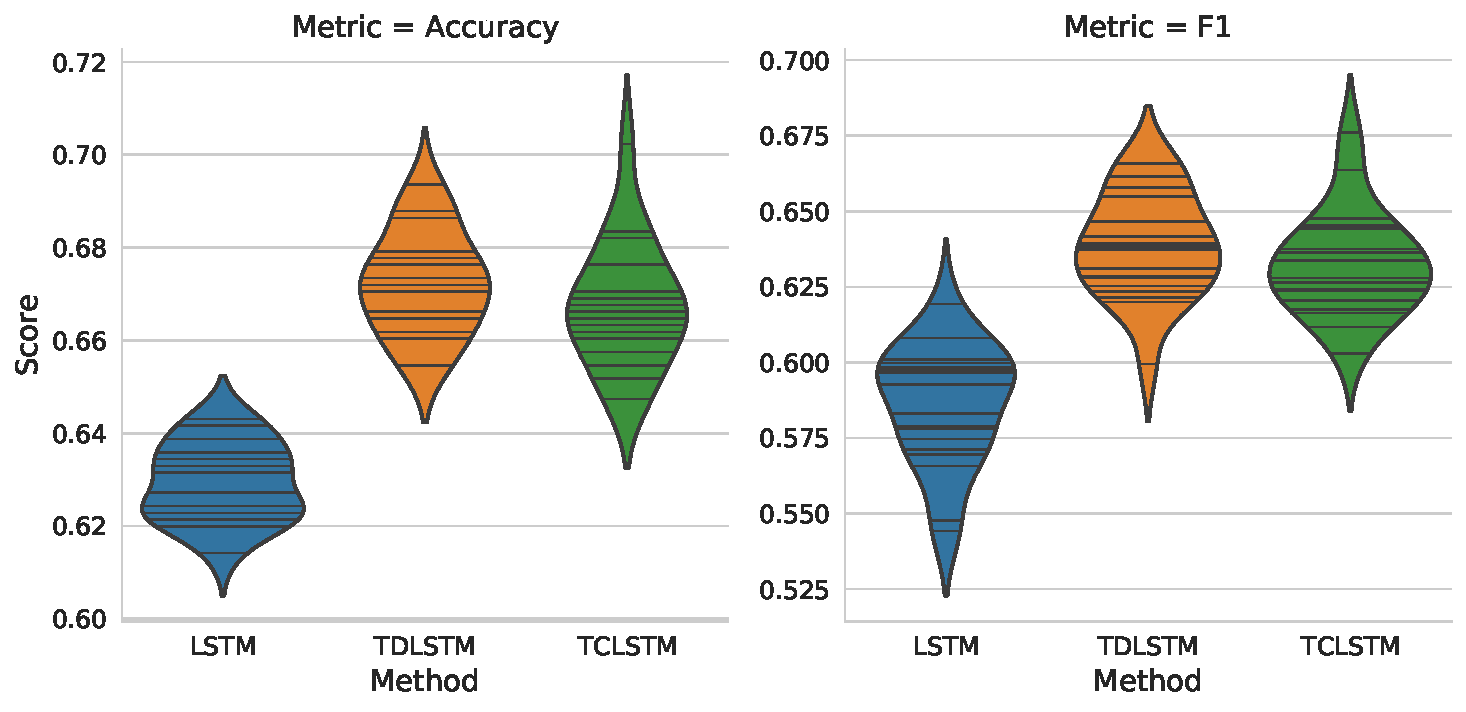
\includegraphics[scale=0.4]{images/reproducibility/tang/LSTM_DIST_ACC_F1.pdf}
    \caption{The distribution of scores for each of the $20$ runs for each reproduced method. Whereby each horizontal line in the distribution represent the result of one run for the reproduced method.}
    \label{fig:repro_tang_LSTM_DIST_ACC_F1}
\end{figure}

\begin{figure}[!h]
    \centering
    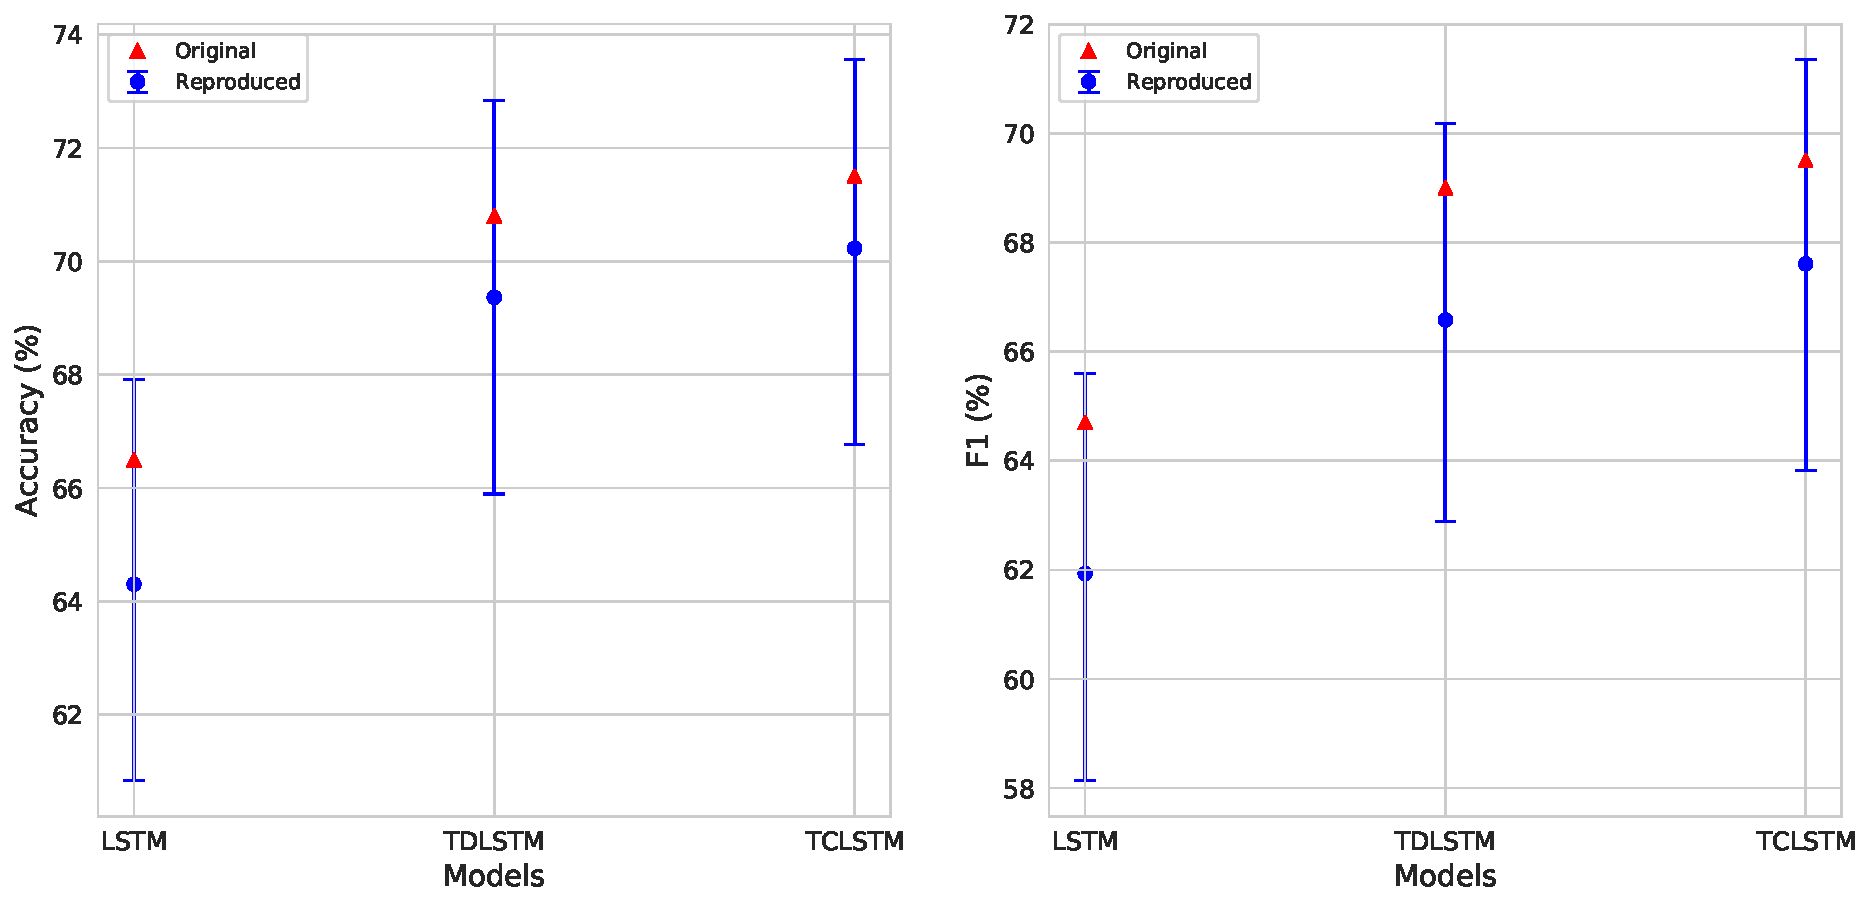
\includegraphics[scale=0.4]{images/reproducibility/tang/LSTM_ACC_F1.pdf}
    \caption{Confidence intervals for the two sided tailed test for the reproduced models of \citet{tang-etal-2016-effective} on both the accuracy and macro F1 metrics.}
    \label{fig:repro_tang_LSTM_ACC_F1}
\end{figure}

Based on the results from table \ref{table:tang_twitter_100_results} it would appear that for many seed values it would not be possible to reproduce these results. To quantify this, the best performing run for each method and metric is compared against all other runs for that method. The number of runs that are significantly worse based on a one sided test corrected using Bonferroni to the best performing run is shown in table \ref{table:tang_significantly_better_runs}. As can be seen out of the $19$ other runs many of them for the macro F1 metric for all methods are significantly different to the best performing run even though they are the same method. This confirms the findings of \citet{reimers-gurevych-2017-reporting} for TDSA for the macro F1 metric whereby random seeds can cause statistically significantly different results for the same method. It further shows that out of all of the methods the TCLSTM would appear to be the least stable, and this could be due to it being the largest, with respect to the number of parameters, of the three methods. From these findings and the distribution of results presented in figure \ref{fig:repro_tang_LSTM_DIST_ACC_F1}, it is believed that a possible reason why others could not reproduce \citep{tay2018learning} or replicate \citep{chen-etal-2017-recurrent} the same scores as the original authors of TDLSTM \citep{tang-etal-2016-aspect} is due to the variance caused by random seeds.

\begin{table}[!h]
    \centering
    \begin{tabular}{|c|c|c|c|}
    \hline
    Metric & LSTM & TDLSTM & TCLSTM  \\
    \hline
    Accuracy & 0 & 0 & 13  \\
    \hline
    F1 & 4 & 2 & 15  \\
    \hline
\end{tabular}
    \caption{The number of runs that the best performing run significantly outperforms using a one side tested and corrected with Bonferroni for accuracy and macro F1.}
    \label{table:tang_significantly_better_runs}
\end{table}

As the methods from \citet{tang-etal-2016-effective} have been reproduced, another of \citet{tang-etal-2016-effective} experiments is repeated and enhanced. The original experiment compares SSWE, GloVe Twitter 50, 100 and 200 embeddings of which both of these embeddings are either type or type and task specific. Thus the experiment is enhanced to include the GloVe 300 dimension non-task nor type specific embedding, that has been already tested in numerous other experiments in this section (see tables \ref{table:repro_vo_word_embeddings_results} and \ref{table:repro_vo_word_embedding_sig_fold_count} for example). The results on the test (validation) set of \citet{dong-etal-2014-adaptive} Twitter dataset can be seen in table \ref{table:repro_tang_test_embedding_scores} (appendix \ref{appendix_reproducibility_tables} table \ref{table:repro_tang_val_embedding_scores}). The findings are slightly different from the original found in figure of \citet{tang-etal-2016-effective}. In comparison \citet{tang-etal-2016-effective} found the TDLSTM to be worse than TCLSTM on all accuracy scores, which is not the case here. Additionally \citet{tang-etal-2016-effective} found SSWE to be worse than GloVe Twitter 50 which again is not found here. These differences in results could be due to the random seeds. More interestingly it is shown that the non-type nor task specific embeddings is better than the all other embeddings for all methods and metrics. Thus showing again that these larger general embeddings can be at least as good as the type and/or task specific embeddings. After performing a one tailed test comparing the GloVe 300 embeddings to all other embeddings for each metric and method they are significantly better in the majority of cases for the test set, as shown in table \ref{table:tang_significantly_better_runs}. The significant results are hard to interpret as the test results suggest that the majority of embeddings for at least TDLSTM and TCLSTM are significantly worse than the GloVe embeddings, but this is not reflected in the validation results as the GloVe embeddings are not significantly better than any of the embeddings\footnote{The p-values from the significant tests can be seen in appendix \ref{appendix_reproducibility_tables} tables \ref{table:repro_tang_embeddings_test_sig} and \ref{table:repro_tang_embeddings_val_sig} for the test and validation results.}. Thus it suggests that perhaps the GloVe embeddings are only weakly better than all other embeddings\footnote{The potential reason for the significance tests to bring back very different results for the test and validation sets could be due to the limitation of the significance test used for the LSTM methods. In this chapter the LSTM based methods when being tested to detect significant differences a particular run from the set of all runs for each compared LSTM method is used. In the majority of cases the median run is used and this to some degree ensures that there is not a bias towards methods that have a large variance in results due to the random seeds. However using the median run or any one run does not take into the account the whole random seed distribution. Thus stating the limitation of the significance test used in this chapter for the LSTM based methods. This limitation could also explain why their is a difference between the significance results of the validation and test set here, as the median run might not be a good representation of all runs results.}.

\begin{table}[!h]
    \centering
    

\begin{tabular}{|c|c|c|c|c|}
\hline
Embedding & Metric &           LSTM &        TDLSTM &        TCLSTM \\
\hline
SSWE & Accuracy &  62.07 \sd{(1.48)} &  66.77$^\star$ \sd{(1.63)} &  65.59$^\star$ \sd{(1.41)} \\
& F1 &  58.37$^\star$ \sd{(2.16)} &  63.35$^\star$ \sd{(1.89)} &  61.96$^\star$ \sd{(1.77)} \\
\hline
Twitter 50 & Accuracy &  61.48$^\star$ \sd{(1.43)} &  65.11$^\star$ \sd{(1.46)} &  64.74$^\star$ \sd{(1.87)} \\
& F1 &  57.12$^\star$ \sd{(2.79)} &  61.67$^\star$ \sd{(2.00)} &  60.72$^\star$ \sd{(2.57)} \\
\hline
Twitter 100 & Accuracy &  62.93 \sd{(0.81)} &  67.23$^\star$ \sd{(1.08)} &  66.74$^\star$ \sd{(1.32)} \\
& F1 &  58.59 \sd{(1.90)} &  63.86$^\star$ \sd{(1.68)} &  63.26$^\star$ \sd{(1.68)} \\
\hline
Twitter 200 & Accuracy &  62.49 \sd{(1.14)} &  68.11$^\star$ \sd{(0.54)} &  67.89 \sd{(0.98)} \\
& F1 &  57.41$^\star$ \sd{(2.81)} &  65.21$^\star$ \sd{(0.94)} &  64.70 \sd{(1.39)} \\
\hline
GloVe 300 & Accuracy &  \textbf{64.73} \sd{(0.76)} &  \textbf{71.04} \sd{(0.68)} &  \textbf{69.22} \sd{(1.27)} \\
& F1 &  \textbf{61.04} \sd{(1.45)} &  \textbf{68.43} \sd{(0.83)} &  \textbf{66.47} \sd{(1.78)} \\
\hline
\end{tabular}
    \caption{Test set mean (standard deviation) results on the \citet{dong-etal-2014-adaptive} Twitter dataset, across various embeddings and methods. The \textbf{bold} values indicate the best embedding score for each method and metric. The $^\star$ indicates when the GloVe embeddings are statistically significantly better (p $\le 0.05$) than the other embedding for that metric and method. The significance test used the one tailed test and used the median best run from the $20$ runs to perform the significance test.}
    \label{table:repro_tang_test_embedding_scores}
\end{table}

\subsection{Conclusion from Reproduction Studies}
It is clear from the large scale NP experiments shown in figures \ref{fig:repro_parameters_c_values_accuracy} (\ref{fig:repro_parameters_c_values_macro_f1}) and \ref{fig:repro_parameters_scaling_accuracy} (\ref{fig:repro_parameters_scaling_macro_f1}) for the accuracy (macro F1) metric, that both the scaling method (if used) and the C-value from the SVM should be stated within the paper. Furthermore the suggestion from \citet{reimers-gurevych-2017-reporting} on reporting multiple runs of the method over different random seed values is required for NN based TDSA methods as the single performance scores can be misleading, which could explain why previous papers obtained different results to the original for the TDLSTM method \citep{chen-etal-2017-recurrent, tay2018learning}. For the first time, it has been shown in this section that scaling method, C-value of the SVM, and random seeds make a significant difference for TDSA methods. 

Additionally within this section it has also been shown that general word embeddings (300 dimension GloVe embeddings) can perform as well as the type and/or task specific embeddings. This has been shown for the NP methods \citep{vo2015target}, where as for the LSTM methods \citep{tang-etal-2016-effective} they tend to prefer the general GloVe embeddings. From this it shows that smaller type and/or task specific embeddings can be as useful as larger general embeddings for at least the NP methods. This implies that from an energy efficiency perspective\footnote{Measured by number of parameters. A better measure for efficiency would be Floating Point Operations (FPO) \citep{schwartz2019green}, but \citet{schwartz2019green} did state that the number of parameters is a form of efficiency measure.} it would be of use to train these smaller type and/or task specific embeddings as the methods that use them will be more efficient than if they use the larger general embeddings. Alternatively it suggests that it is not a requirement to create smaller type and/or task specific embeddings. These findings are at least true for TDSA methods applied to the Dong dataset.

\section[Mass Evaluation]{Mass Evaluation\footnote{Within this section the TDParse Plus and Target Dependent Plus methods will also be called TDParse+ and TD+ respectively.}}
\label{section:repro_mass_eval}
% Need to mention here the difference in the datasets in more detail e.g. dataset size etc macro F1 results etc etc

% Furthermore two of the three methods \citep{vo2015target, tang-etal-2016-effective} that were originally only evaluated on Dong dataset were therefore only evaluated on data that contains one target per text, as shown by the ATS value in table \ref{table:repro_dataset_stats}. 

Given the methods from the three reproduced papers, in this section we evaluate the different methods across six different English datasets that are shown in table \ref{table:repro_dataset_stats}. This will be the first TDSA study that has evaluated methods across different types, mediums, and domains, as well as the largest TDSA evaluation with respect to the number of datasets. This study will thus explore whether the three papers' methods perform differently on these various datasets, seeing if any generalise to all datasets. For all methods they will use the same 300 dimension GloVe embedding as it is the most popular and has been shown within the thesis to perform well on data that it was not originally designed for (i.e. social media type data). All methods will use the Spacy tokeniser and the \citet{wang-etal-2017-tdparse} methods will use the TweeboParser \citep{kong-etal-2014-dependency} dependency parser on all datasets\footnote{This is due to the methods requirements of a dependency parser that produces multiple roots.}. For sentiment lexicon based methods, the same lexicons that \citet{wang-etal-2017-tdparse} employed will be used here. For the NP methods, the best performing C-value for each method and dataset for the accuracy metric found through the experiment conducted in figure \ref{fig:repro_parameters_c_values_accuracy} will be used. Also MinMax scaling will be used for all NP methods. The LSTM based methods will use the same setup as that from section \ref{section:repro_lstm}, but the methods will only be run six times for each dataset due to the computational cost\footnote{Six runs was chosen as according to \citet{reimers2018comparing} as it will allow future researches to compare results using significance tests that take all six runs into account. This test was not used in this chapter as neural methods that require running multiple runs are compared to non-neural methods that do not, and there is no literature that is known to the author that states how to compare multiple run performances to single run performances.}. Further, for all of the LSTM methods the mean result from the six runs will be reported unless otherwise stated. For the NP methods only the two top performing methods are evaluated, again to save on computational cost while still allowing us to compare methods that do and do not use sentiment lexicons. 

% That the addition of sentiment lexicons does not help that much nor does the dependency parser.
The accuracy and macro F1 results on the test set for all datasets can be seen in tables \ref{table:repro_mass_eval_acc} and \ref{table:repro_mass_eval_macro_f1}. The statistically significant results comparing each method can be seen for both metrics in figure \ref{figure:repro_mass_eval_test_sig_results}, for the LSTM methods the median best performing run based on the accuracy metric is used to compare to all other methods. From these results it is clear that the NP methods are by far the better set of methods. Additionally it can be seen that adding sentiment lexicons (NP methods with a `+' in their name) only marginally improve results on some datasets and at most significantly better on one dataset. These findings are also similar when comparing the non-dependency parser approaches (TD and TD+ methods) with those that do use a dependency parser (TDParse and TDParse+), whereby they perform almost as well as each other. Both of these findings show, for at least the methods tested here, that using additional resources such as sentiment lexicons or a dependency parser do not make a large significant difference in results and are thus not needed.

\begin{table}[!h]
    \centering
    
\begin{tabular}{|c|c|c|c|c|c|c|c|}
  \hline
  &   D &  E &  L &  M &  R &  Y &   Mean \\
 \hline
LSTM &  \underline{64.57} &     \underline{47.85} &   59.90 &     71.04 &       \underline{68.63} &      \underline{63.33} &  \underline{62.55} \\
 \hline
TDLSTM &  \textbf{71.12} &     \textbf{57.50} &   61.76 &     \underline{70.52} &       73.56 &      64.17 &  66.44 \\
  \hline
TCLSTM &  68.98 &     57.40 &   \underline{56.77} &     70.77 &       71.85 &      66.81 &  65.43 \\
   \hline
TD &  68.50 &     57.22 &   66.14 &     73.45 &       77.32 &      82.50 &  70.86 \\
   \hline
TD+ &  70.23 &     53.21 &   \textbf{68.97} &     \textbf{74.37} &       78.04 &      81.67 &  71.08 \\
    \hline
TDParse &  67.77 &     57.46 &   67.08 &     73.96 &       77.95 &      79.58 &  70.63 \\
    \hline
TDParse+ &  69.36 &     56.12 &   68.50 &     73.35 &       \textbf{78.30} &      \textbf{83.33} &  \textbf{71.49} \\
\hline
Mean &  68.65 &     55.25 &   64.16 &     72.49 &       75.09 &      74.48 &  - \\
\hline
\multicolumn{8}{|p{11.5cm}|}{\centering D=Dong, E=Election, L=Laptop, M=Mitchell, R=Restaurant, Y=YouTuBean}\\
\hline
\end{tabular}
    \caption{Accuracy results on the test sets of each dataset. For the LSTM based methods this is the mean accuracy result. The mean accuracy across all datasets for each method is in the right most column. Where the \textbf{bold} and \underline{underlined} values indicate the best and worst methods for each dataset and the overall mean accuracy, respectively. The mean accuracy score for each dataset is in the last row.}
    \label{table:repro_mass_eval_acc}
\end{table}

\begin{table}[!h]
    \centering
    \begin{tabular}{|c|c|c|c|c|c|c|c|}
  \hline
  &   D &  E &  L &  M &  R &  Y &   Mean \\
 \hline
 LSTM &  \underline{61.58} &     \underline{30.65} &   \underline{41.91} &     35.51 &       \underline{37.15} &      \underline{25.85} &  \underline{38.78} \\
 \hline
 TDLSTM &  \textbf{68.54} &     42.54 &   49.82 &     \underline{29.67} &       56.66 &      28.98 &  46.04 \\
 \hline
 TCLSTM &  65.92 &     43.57 &   45.04 &     38.42 &       53.54 &      36.83 &  47.22 \\
 \hline
 TD &  65.27 &     46.60 &   57.86 &     48.98 &       63.17 &      \textbf{74.80} &  59.45 \\
 \hline
 TD+ &  67.36 &     44.52 &   \textbf{62.33} &     48.08 &       64.44 &      72.90 &  59.94 \\
 \hline
 TDParse &  64.33 &     \textbf{46.64} &   59.23 &     48.58 &       64.66 &      70.05 &  58.91 \\
 \hline
 TDParse+ &  66.36 &     46.30 &   61.89 &     \textbf{51.17} &       \textbf{65.26} &      74.46 &  \textbf{60.91} \\
 \hline
 Mean &  65.62 &     42.98 &   54.01 &     42.92 &       57.84 &      54.84 &  - \\
 \hline
\multicolumn{8}{|p{11.5cm}|}{\centering D=Dong, E=Election, L=Laptop, M=Mitchell, R=Restaurant, Y=YouTuBean}\\
\hline
 \end{tabular}
    \caption{Macro F1 results on the test sets of each dataset. For the LSTM based methods this is the mean macro F1 result. The mean macro F1 across all datasets for each method is in the right most column. Where the \textbf{bold} and \underline{underlined} values indicate the best and worst methods for each dataset and the overall mean macro F1, respectively. The mean macro F1 score for each dataset is in the last row.}
    \label{table:repro_mass_eval_macro_f1}
\end{table}

\begin{figure}[!h]
    \centering
    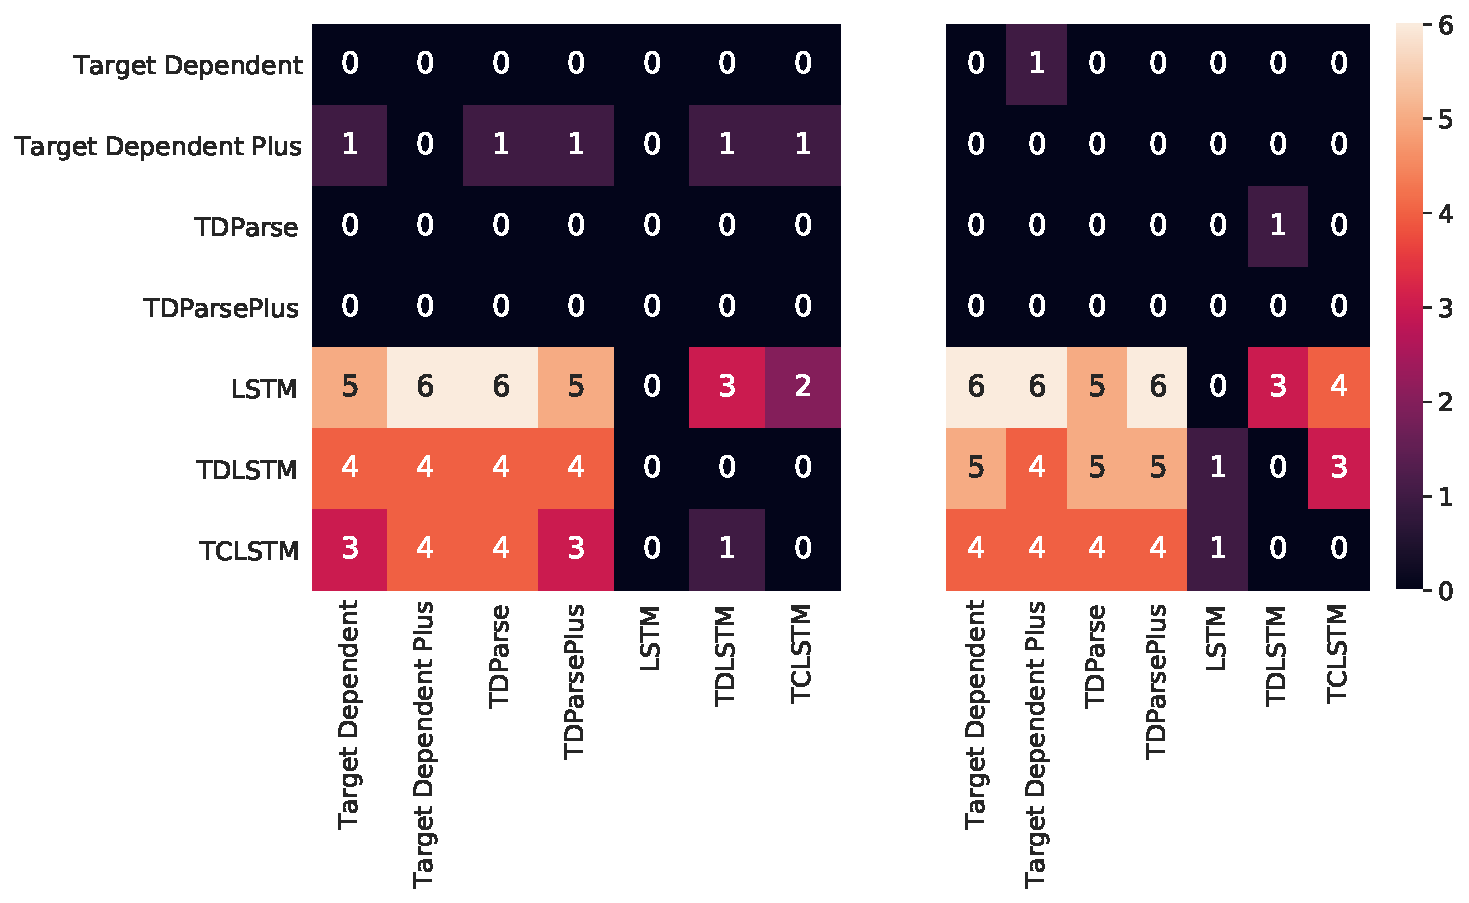
\includegraphics[scale=0.4]{images/reproducibility/Sig_Test.pdf}
    \caption{The number of datasets where the column methods are statistically significantly better than the row methods, corrected using Bonferroni. The left and right heatmap represent the accuracy and macro F1 scores. This is using the median performing run based on the accuracy metric for the LSTM methods.}
    \label{figure:repro_mass_eval_test_sig_results}
\end{figure}

% It has been shown that some of the LSTM methods perform worse than the baseline sentence method.
Between the LSTM based methods it is clear that on average the target specific LSTM based methods (TDLSTM and TCLSTM) are better than the sentence level classifier baseline (LSTM). However the TDLSTM and TCLSTM are worse than the LSTM on the Mitchell dataset, and the TCLSTM is worse than LSTM on the Laptop dataset when using the accuracy metric. Both of these represent a failure for the target specific methods as they are beaten by a much simpler baseline. This finding demonstrates one reason why it is important to test methods across a wide range of datasets.

% LSTM methods perform worse when low resourced or highly unbalanced.
Comparing the LSTM based methods to the NP it is clear that the LSTM based methods perform better in comparison to NP on larger datasets e.g. Election and Dong. Whereas the NP methods in comparison perform much better on the smaller datasets (YouTuBean), further they also perform better with respect to macro F1 scores. The macro F1 results suggest that the LSTM methods perform poorly on datasets that are highly un-balanced e.g. Mitchell and this gets worse when the dataset is small and un-balanced e.g. YouTuBean. Furthermore for the YouTuBean and the Mitchell datasets the macro F1 score distribution is quite large, as shown in figure \ref{figure:repro_LSTM_TEST_F1}\footnote{For the distribution of the accuracy scores for the LSTM methods see figure \ref{figure:repro_LSTM_TEST_ACC} in appendix \ref{appendix_reproducibility_images}.}, in comparison to all of the other datasets. This suggests that the LSTM methods are more sensitive to random seed/initialisation for smaller and un-balanced datasets. To overcome the overfitting to particular labels, re-sampling techniques such as under or over sampling could be of use. In some prior work it has been shown that transfer learning from a document sentiment dataset has greatly improved the macro F1 score for LSTM methods \citep{he-etal-2018-exploiting}. However more work investigating how to improve NN based TDSA methods with respect to highly un-balanced and/or low resourced corpora should be investigated. Lastly from the significance results it is clear that the NP methods do not struggle to beat the LSTM sentence level classifier baseline.

\begin{figure}[!h]
    \centering
    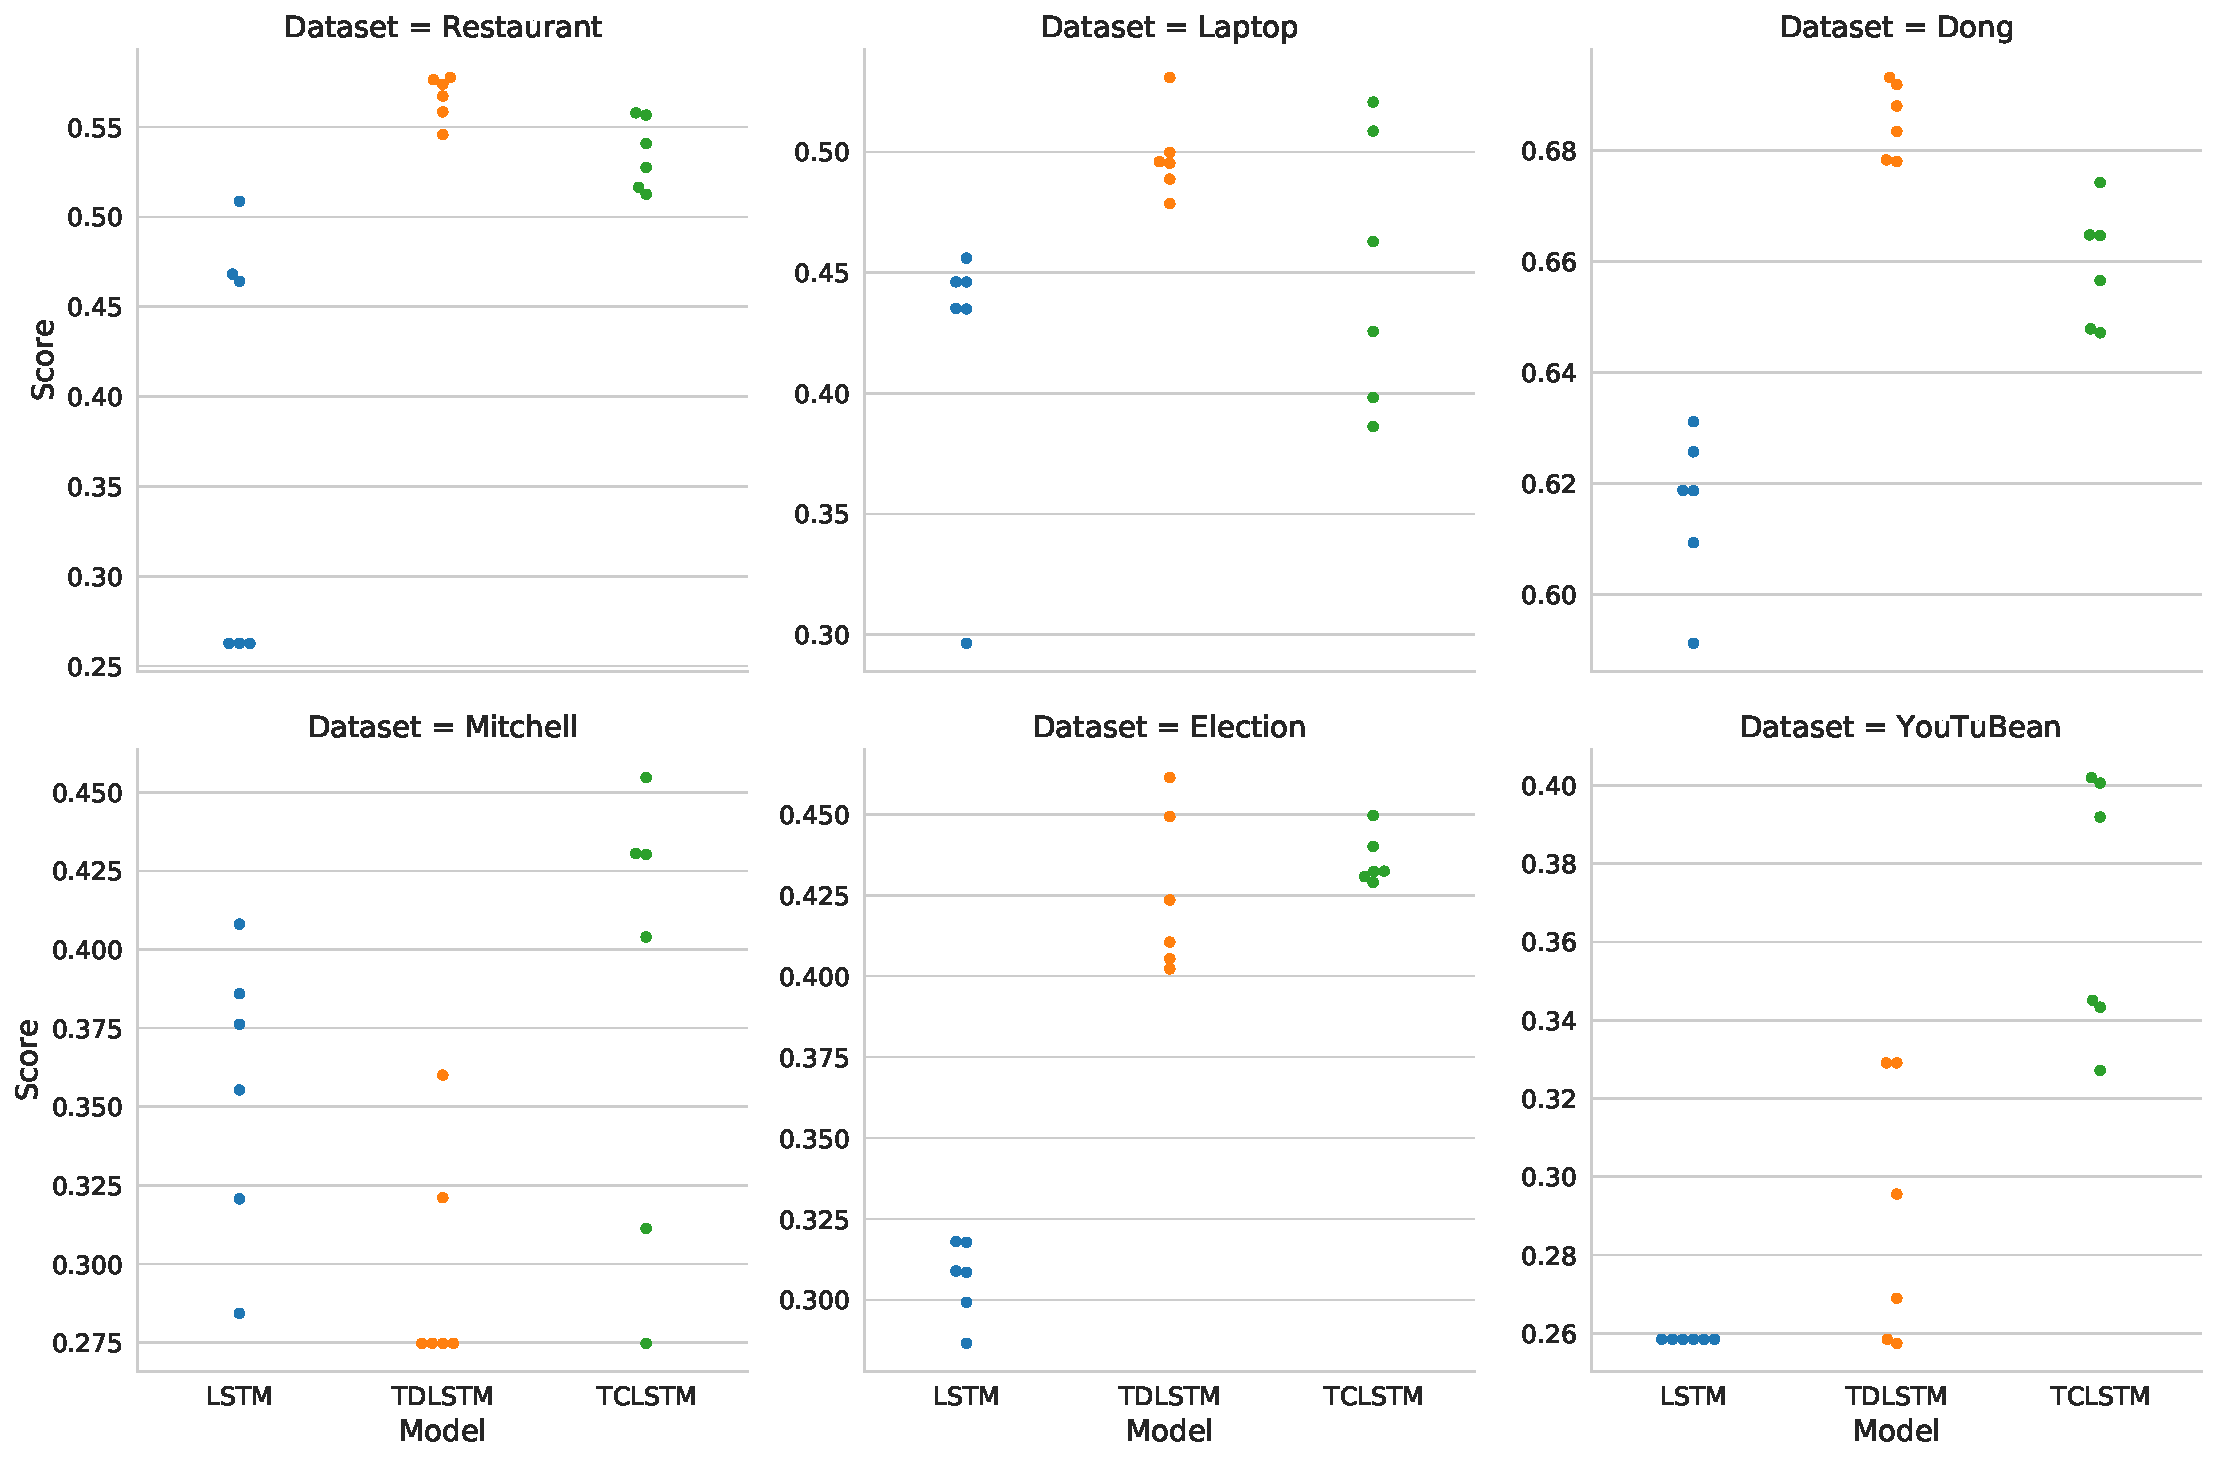
\includegraphics[scale=0.3]{images/reproducibility/LSTM_Test_F1.pdf}
    \caption{Distribution of macro F1 scores from the six runs for each LSTM method and test dataset.}
    \label{figure:repro_LSTM_TEST_F1}
\end{figure}

% Stating that the variation in datasets, that it would appear that the methods are more affected by size, DS, and class distribution rather than type, medium, and domain
From a performance perspective in general the hardest dataset, according to accuracy, is the Election one, even though it is the largest by a large margin. The reason for its difficulty is believed to stem from the fact it has a large distribution of samples in $DS_2$ and $DS_3$, as \citet{wang-etal-2017-tdparse} suggest that $DS_3$ is the most difficult scenario. It also appears that the methods are less affected by the type, domain, or medium that dataset has come from but rather the size, \textit{DS} distribution, and sentiment class distribution. This is observed as methods that do incorporate type specific features e.g. a Twitter based dependency parser perform worse in rank terms on the social media type datasets some of the time than on the non-social media type datasets. For example, TDParse performs worse on Dong but better on Laptop compared to TD.

% Showing that by using a better seed value the LSTM methods are stil worse.
It is worth noting that to a large extent the NP methods have an advantage over the LSTM methods as the C-value which is significant has been tuned for each dataset and method, where as the LSTM methods have had no tuning. However some of the NP methods still perform better than the TDLSTM results for the Restaurant dataset from prior work, as shown by table \ref{table:repro_tang_authors_differences}. This is highlighted as these other prior works may have tuned the TDLSTM or found a better seed value than in the evaluation performed here. To give the LSTM methods an increased advantage over the NP methods, due to the NP methods having their C-values tuned, the LSTM methods have been recompared to the NP whereby the best performing run/seed value is used. Figures \ref{figure:repro_mass_eval_max_acc_test_sig_results} and \ref{figure:repro_mass_eval_max_f1_test_sig_results} show the number of datasets that the methods are significantly better on using the best performing run based on the accuracy and macro F1 metric. However with this increased advantage for the LSTM methods it can be seen that the NP methods are still significantly better and the change in the heatmap compared to figure \ref{figure:repro_mass_eval_test_sig_results} is minimal. 

\begin{figure}[!h]
    \centering
    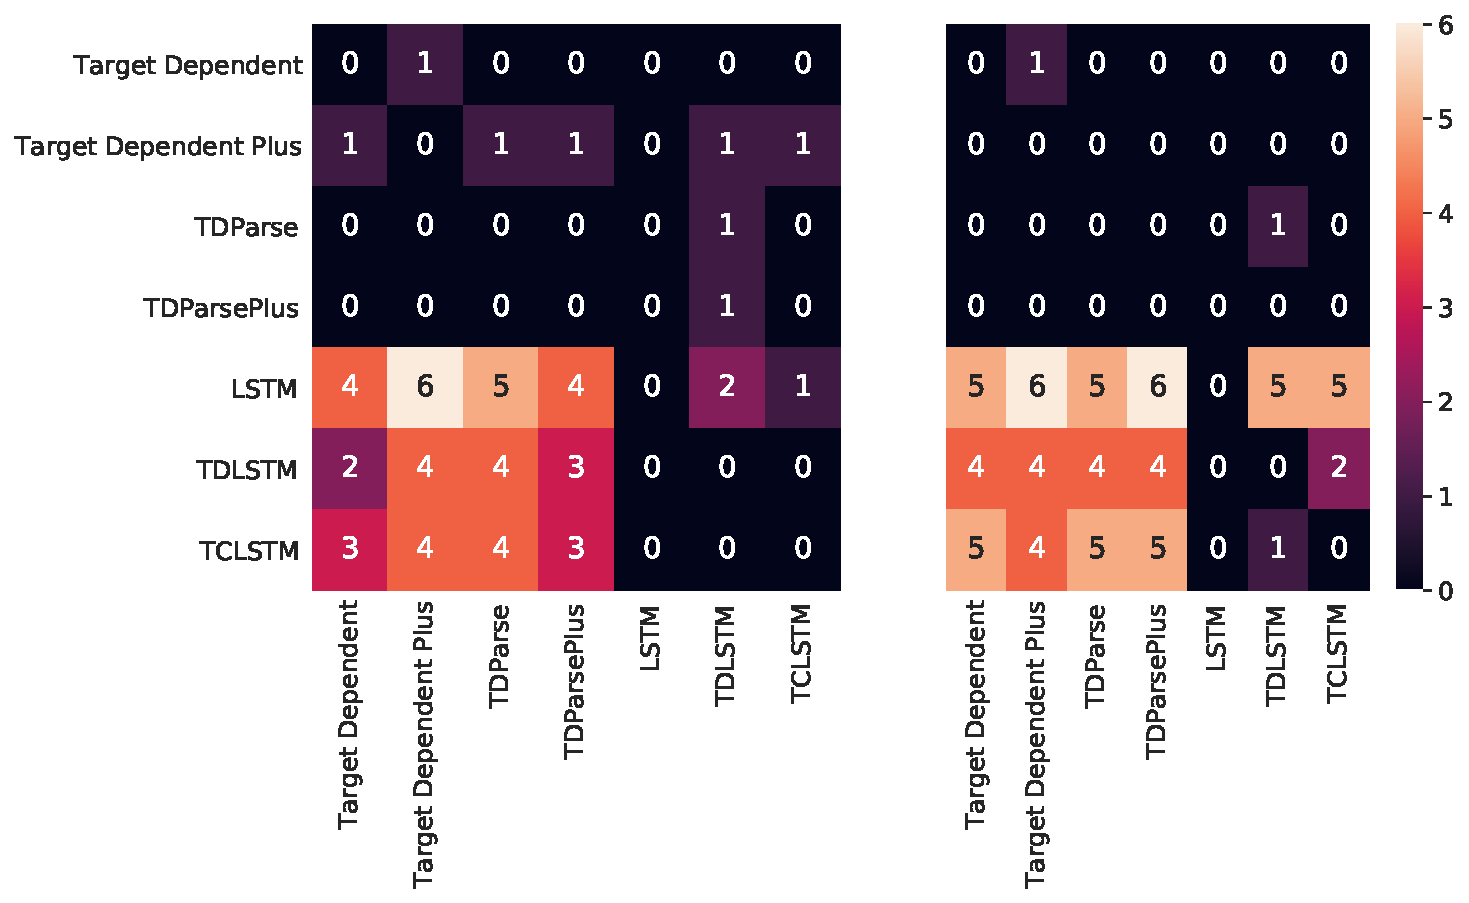
\includegraphics[scale=0.4]{images/reproducibility/Sig_Max_Acc_Test.pdf}
    \caption{The number of datasets where the column methods are statistically significantly better than the row methods, corrected using Bonferroni. The left and right heatmaps represent the accuracy and macro F1 scores. This is using the best performing run based on the \textbf{accuracy metric} for the LSTM methods.}
    \label{figure:repro_mass_eval_max_acc_test_sig_results}
\end{figure}

\begin{figure}[!h]
    \centering
    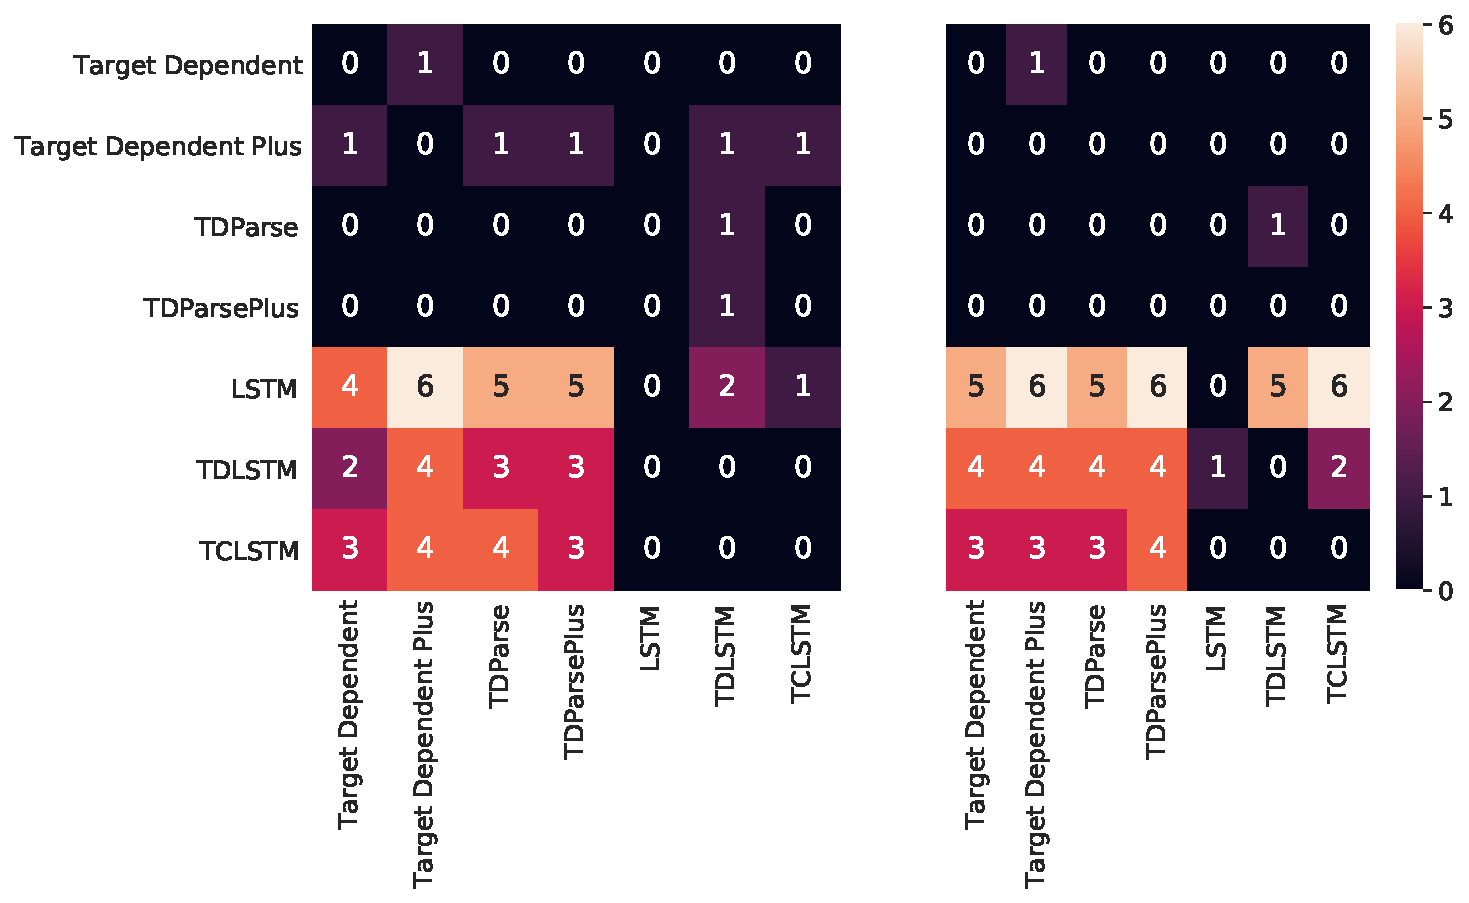
\includegraphics[scale=0.4]{images/reproducibility/Sig_Max_F1_Test.pdf}
    \caption{The number of datasets where the column methods are statistically significantly better than the row methods, corrected using Bonferroni. The left and right heatmaps represent the accuracy and macro F1 scores. This is using the best performing run based on the \textbf{macro F1 metric} for the LSTM methods.}
    \label{figure:repro_mass_eval_max_f1_test_sig_results}
\end{figure}

As stated earlier, the LSTM methods tend to perform worse on smaller datasets. Thus to test how this low resource setting affects LSTM and NP methods on a larger scale all of the datasets training set sizes have been reduced to the same size as YouTuBean training set size, which is the smallest dataset within the evaluated datasets\footnote{For the \citet{dong-etal-2014-adaptive} Twitter dataset instead of training the NP methods using the median pooled approach due to the `same target multiple appearance' issue \citet{wang-etal-2017-tdparse}. All methods including the NP methods will use the first appearance of the target in the text. This was done due to compatibility reason between the NP and LSTM methods after splitting the training dataset.}. Further for the LSTM based methods this new reduced training set size also means that 20\% of that training set is used as a validation set for early stopping. All methods are retrained using the same settings. As the YouTuBean dataset has already been evaluated and would not be affected by this new size reduction it will not be included in the analysis of these experiments. The accuracy and macro F1 results on the test sets for these datasets can be seen in tables \ref{table:repro_small_mass_eval_acc} and \ref{table:repro_small_mass_eval_macro_f1}. The statistically significant results comparing each method can be seen for both metrics in figure \ref{figure:repro_mass_eval_small_test_sig_results}, for the LSTM methods the median best performing run based on the accuracy metric is used to compare to all other methods.

% It can be seen in this more low resourced setting that the sentiment lexicons do appear to be beneifical within the review domain. This is probably because the Hu and Liu sentiments are form the review type

\begin{table}[!h]
    \centering
    \begin{tabular}{|c|c|c|c|c|c|c|}
\hline
Method  &   D &  E &  L &  M &  R  &   Mean \\
\hline
LSTM &  \underline{50.00} &     \underline{46.20} &   53.11 &     \underline{70.11} &       \underline{65.00} &  \underline{56.88} \\
\hline  
TDLSTM &  50.02 &     49.00 &   52.25 &     \underline{70.11} &       \underline{65.00} &  57.28 \\
\hline  
TCLSTM &  51.01 &     49.91 &   \underline{50.89} &     \underline{70.11} &       \underline{65.00} &  57.39 \\
\hline   
TD &  65.75 &     \textbf{51.59} &   60.82 &     \textbf{72.75} &       72.50 &  64.68 \\
\hline    
TD+ &  \textbf{66.62} &     49.08 &   \textbf{64.58} &     72.64 &       74.29 &  65.44 \\
\hline    
TDParse &  65.61 &     \textbf{51.59} &   60.82 &     72.44 &       74.11 &  64.91 \\
\hline    
TDParse+ &  65.75 &     50.45 &   64.26 &     71.94 &       \textbf{74.91} &  \textbf{65.46} \\
\hline
Mean &  59.25 &     49.69 &   58.10 &     71.44 &       70.11 &  - \\
\hline
\multicolumn{7}{|p{9.5cm}|}{\centering D=Dong, E=Election, L=Laptop, M=Mitchell, R=Restaurant, Y=YouTuBean}\\
\hline
\end{tabular}
    \caption{Using the smaller training datasets, the accuracy results on the test sets of each dataset. For the LSTM based methods this is the mean accuracy result. The mean accuracy across all datasets for each method is in the right most column. Where the \textbf{bold} and \underline{underlined} values indicate the best and worst methods for each dataset and the overall mean accuracy, respectively. The mean accuracy score for each dataset is in the last row.}
    \label{table:repro_small_mass_eval_acc}
\end{table}

\begin{table}[!h]
    \centering
    \begin{tabular}{|c|c|c|c|c|c|c|}
\hline
Method  &   D &  E &  L &  M &  R  &   Mean \\
\hline
LSTM &  \underline{22.22} &     27.15 &   \underline{23.47} &     \underline{27.48} &       \underline{26.26} &  \underline{25.32} \\
\hline
TDLSTM &  22.29 &     \underline{26.14} &   29.12 &     \underline{27.48} &       \underline{26.26} &  26.26 \\
\hline
TCLSTM &  27.65 &     32.46 &   32.59 &     \underline{27.48} &       \underline{26.26} &  29.29 \\
\hline
TD &  \textbf{62.48} &     39.18 &   52.11 &     \textbf{45.73} &       54.66 &  50.83 \\
\hline
TD+ &  62.44 &     39.34 &   \textbf{57.71} &     41.41 &       58.65 &  51.91 \\
\hline
TDParse &  62.43 &     \textbf{39.39} &   51.69 &     44.14 &       57.77 &  51.08 \\
\hline
TDParse+ &  61.36 &     38.25 &   56.86 &     44.58 &       \textbf{60.14} &  \textbf{52.24} \\
\hline
Mean &  45.84 &     34.56 &   43.36 &     36.90 &       44.29 &  - \\
\hline
\multicolumn{7}{|p{9.5cm}|}{\centering D=Dong, E=Election, L=Laptop, M=Mitchell, R=Restaurant, Y=YouTuBean}\\
\hline
\end{tabular}
    \caption{Using the smaller training datasets, the macro F1 results on the test sets of each dataset. For the LSTM based methods this is the mean macro F1 result. The mean macro F1 across all datasets for each method is in the right most column. Where the \textbf{bold} and \underline{underlined} values indicate the best and worst methods for each dataset and the overall mean macro F1, respectively. The mean macro F1 score for each dataset is in the last row.}
    \label{table:repro_small_mass_eval_macro_f1}
\end{table}

\begin{figure}[!h]
    \centering
    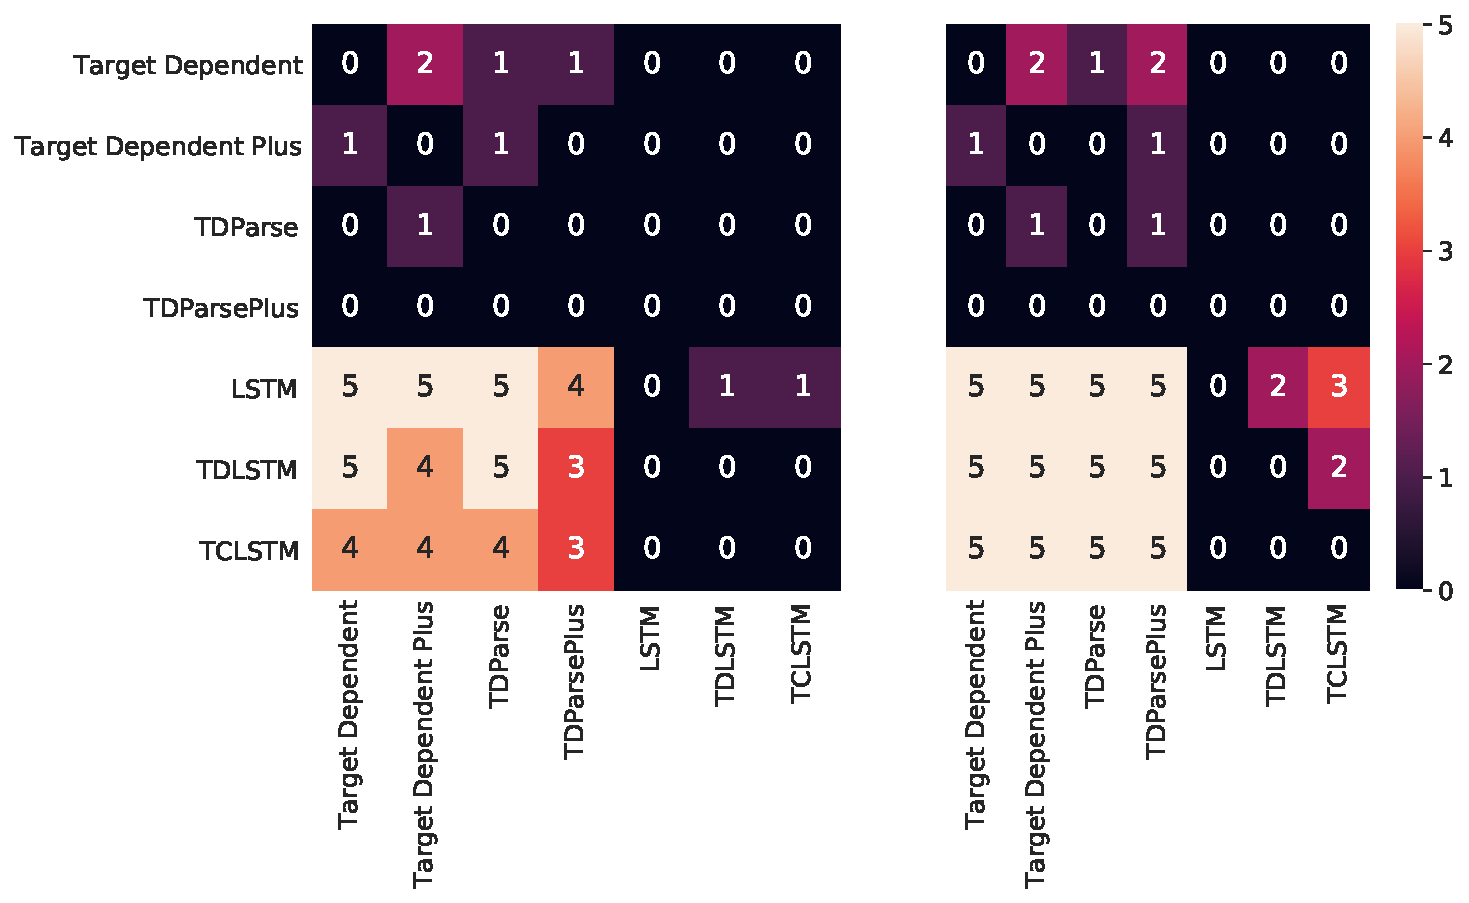
\includegraphics[scale=0.4]{images/reproducibility/Small_Sig_Test.pdf}
    \caption{Using the smaller training datasets, the values represent number of datasets the column methods are statistically significantly better than the row methods, corrected using Bonferroni. The left and right heatmap represent the accuracy and macro F1 scores. This is using the median performing run based on the accuracy metric for the LSTM methods.}
    \label{figure:repro_mass_eval_small_test_sig_results}
\end{figure}

% In the low resource setting it is more clear that the NP methods perform a lot better. Furthermore they do not overfit to only one sentiment class. Also it is more clear that the sentiment lexicons are more affective in the low resource setting if the lexicon used is close to the dataset applied on.
From the results it is clear that the NP methods perform the best in this low resource setting. The datasets that the LSTM methods did perform better on (Dong and Election), they are now worse on. The target specific LSTM methods (TDLSTM and TCLSTM) now have very similar performance to the sentence level LSTM method, which was not the case for all of the results in the normal resource setting. Furthermore the LSTM methods have exceptionally poor performance on the macro F1 results, so much so that all NP methods are significantly better on all datasets compared to all of the LSTM methods. The macro F1 results are broken down into F1 scores for each of the sentiment classes positive, neutral, and negative which can be see in tables \ref{table:repro_small_mass_eval_pos_f1}, \ref{table:repro_small_mass_eval_neu_f1}, and \ref{table:repro_small_mass_eval_neg_f1}. From these results it is clear that for the datasets that are most un-balanced, the LSTM methods can only predict the majority class correctly e.g neutral for Mitchell and positive for Restaurant. In comparison the NP methods are much less affected by the un-balanced datasets and can predict at least one sample correctly for all sentiment classes for all datasets, which only the TCLSTM method can do for the Laptop and Dong dataset. 

In the low resource setting for NP methods, it is still clear that the addition of a dependency parser (TDParse and TDParse+)  does not make a large significance difference. In comparison it is more clear that for the dataset from the written medium and coming from the review domain (Laptop and Restaurant) that using sentiment lexicons makes a large difference for both the accuracy and macro F1 metrics. This result is most likely due to the limited data and thus the sentiment lexicon act as a good inductive bias. The reason why the lexicon based methods perform well only on these datasets is most likely due to one of the lexicons coming from that medium and type, \citet{hu2004mining} sentiment lexicon, where as the other lexicons used are more general. This shows that in a low resource setting sentiment lexicons are useful, only if they come from the same type and medium, as the YouTuBean which comes from the review type but not written medium does not benefit from the sentiment lexicons as shown in table \ref{table:repro_mass_eval_acc} and \ref{table:repro_mass_eval_macro_f1}\footnote{For the TDParse method there is an increase for both the accuracy and macro F1 metric when adding sentiment lexicon. This is not the case for the TD method whereby adding sentiment lexicons harms the performance for both accuracy and macro F1.}.

\begin{table}[!h]
    \centering
    \begin{tabular}{|c|c|c|c|c|c|c|}
\hline
Method  &   D &  E &  L &  M &  R  &   Mean \\
\hline
LSTM &   \underline{0.00} &      \underline{0.00} &   \underline{69.43} &      \underline{0.00} &       \underline{78.79} &  \underline{29.64} \\
\hline
TDLSTM &   \underline{0.00} &      \underline{0.00} &   70.53 &      \underline{0.00} &       \underline{78.79} &  29.86 \\
\hline
TCLSTM &  10.40 &      \underline{0.00} &   70.28 &      \underline{0.00} &       \underline{78.79} &  31.89 \\
\hline
TD &  57.88 &      6.38 &   76.73 &     \textbf{41.40} &       84.00 &  \textbf{53.28} \\
\hline
TD+ &  54.23 &     \textbf{12.43} &   78.79 &     31.40 &       84.96 &  52.36 \\
\hline
TDParse &  \textbf{58.20} &      6.83 &   76.82 &     38.30 &       84.57 &  52.94 \\
\hline
TDParse+ &  52.63 &      5.87 &   \textbf{79.31} &     38.35 &       \textbf{85.17} &  52.27 \\
\hline
\end{tabular}
    \caption{Using the smaller training datasets, the F1 results for the \textbf{positive class} on the test sets of each dataset. For the LSTM based methods this is the mean F1 result. The mean F1 across all datasets for each method is in the right most column. Where the \textbf{bold} and \underline{underlined} values indicate the best and worst methods for each dataset and the overall mean F1, respectively.}
    \label{table:repro_small_mass_eval_pos_f1}
\end{table}

\begin{table}[!h]
    \centering
    \begin{tabular}{|c|c|c|c|c|c|c|}
\hline
Method  &   D &  E &  L &  M &  R  &   Mean \\
\hline
LSTM &  \underline{66.67} &     20.71 &    \underline{0.00} &     \underline{82.43} &        \underline{0.00} &  33.96 \\
\hline
TDLSTM &  66.69 &     \underline{13.70} &   \underline{0.00} &     \underline{82.43} &        \underline{0.00} &  \underline{32.56} \\
\hline
TCLSTM &  67.02 &     34.57 &    0.39 &     \underline{82.43} &        \underline{0.00} &  36.88 \\
\hline
TD &  72.87 &     52.06 &   33.62 &     83.68 &       31.91 &  54.83 \\
\hline
TD+ &  \textbf{73.99} &     48.45 &   \textbf{42.80} &     \textbf{83.74} &       37.54 &  \textbf{57.31} \\
\hline
TDParse &  72.41 &     \textbf{52.79} &   31.62 &     83.38 &       33.21 &  54.68 \\
\hline
TDParse+ &  73.37 &     50.98 &   41.11 &     83.15 &       \textbf{37.67} &  57.26 \\
\hline
\end{tabular}
    \caption{Using the smaller training datasets, the F1 results for the \textbf{neutral class} on the test sets of each dataset. For the LSTM based methods this is the mean F1 result. The mean F1 across all datasets for each method is in the right most column. Where the \textbf{bold} and \underline{underlined} values indicate the best and worst methods for each dataset and the overall mean F1, respectively.}
    \label{table:repro_small_mass_eval_neu_f1}
\end{table}

\begin{table}[!h]
    \centering
    \begin{tabular}{|c|c|c|c|c|c|c|}
\hline
Method  &   D &  E &  L &  M &  R  &   Mean \\
\hline
LSTM &   \underline{0.00} &     60.75 &    \underline{1.00} &      \underline{0.00} &        0.00 &  \underline{12.35} \\
\hline
TDLSTM &   0.19 &     \textbf{64.72} &   16.82 &      \underline{0.00} &        \underline{0.00} &  16.34 \\
\hline
TCLSTM &   5.54 &     62.81 &   27.09 &      \underline{0.00} &        \underline{0.00} &  19.09 \\
\hline
TD &  56.70 &     59.11 &   45.97 &     12.12 &       48.05 &  44.39 \\
\hline
TD+ &  \textbf{59.09} &     \underline{57.14} &   \textbf{51.53} &      9.09 &       53.46 &  46.06 \\
\hline
TDParse &  56.68 &     58.54 &   46.63 &     10.75 &       55.52 &  45.62 \\
\hline
TDParse+ &  58.09 &     57.90 &   50.15 &     \textbf{12.24} &       \textbf{57.58} &  \textbf{47.19} \\
\hline
\end{tabular}
    \caption{Using the smaller training datasets, the F1 results for the \textbf{negative class} on the test sets of each dataset. For the LSTM based methods this is the mean F1 result. The mean F1 across all datasets for each method is in the right most column. Where the \textbf{bold} and \underline{underlined} values indicate the best and worst methods for each dataset and the overall mean F1, respectively.}
    \label{table:repro_small_mass_eval_neg_f1}
\end{table}

\section{Conclusion}
Within this chapter, the reproduction studies have found, for the first time, that for NP methods within TDSA both scaling features and C-values within SVMs are statistically significant factors. Furthermore it is recommended that these factors are reported within a structured format like that suggested by \citet{dodge-etal-2019-show} within Appendix B-D with all other relevant information about the method. For TDSA LSTM based methods it has been shown for at least one metric (macro F1) that they can be statistically significantly affected by random seeds for the first time, this has been shown previously by \citet{reimers-gurevych-2017-reporting} for neural sequence labelling methods. Thus it is recommended to follow \citet{reimers-gurevych-2017-reporting} advice on reporting and comparing distribution of scores that are generated from the LSTM methods by different random seeds. 

Additionally the reproduction studies found that for NP the larger general embedding (300 dimension GloVe) can perform as well as the type and/or task specific embeddings that the original method used \citep{vo2015target}. This implies that from an energy saving perspective it can be useful to train smaller more relevant embeddings for NP methods. While the LSTM methods preferred the larger general embedding, suggesting there is no requirement to train smaller more relevant embeddings. However these findings have only been tested on NP and LSTM methods on one Twitter dataset (Dong \citep{dong-etal-2014-adaptive}), it would be beneficial to broaden the experiment to more datasets. These findings so far in the conclusion have allowed us to answer \rqref{rq:lessons} `what lesson can be learned from reproducing a method within TDSA?’.

The following findings help to answer \rqref{rq:generalisable} `how generalisable are existing methods within TDSA?'. It is found that in general the NP methods are better than the LSTM, but the LSTM methods can perform better in general on larger datasets. Thus showing to some degree that there is no one winning method. While testing methods across various datasets that have different domains, types, and mediums it is found that on the standard datasets sizes these factors do not differentiate the methods. Rather, testing methods on datasets that vary by size, sentiment class distribution, and Distinct Sentiment (\textit{DS}) distribution are the most influential factors. From these factors it is shown that in general all methods perform badly when the dataset contains a large distribution of samples from $DS_3$ and $DS_2$. Further the LSTM methods are badly affected when the datasets are highly un-balanced and/or small, in these cases the NP methods are highly recommend. It was found in the low resource setting, that the inductive bias of sentiment lexicons in NP methods is useful, only if the sentiment lexicon comes from the same type and medium. Neither, the use of sentiment lexicons nor the features from a dependency parser are of significant use in the higher resource setting. Lastly it was found in some cases the target specific methods (TDLSTM and TCLSTM) were no better than the baseline (LSTM) method. This was not found in the original paper \citep{tang-etal-2016-effective}, as the datasets this was found on was not used by the original paper, demonstrating the need to test methods across varying datasets. From these findings it is recommended that future work investigates how to improve TDSA methods within the low resource and/or unbalanced setting especially for NN/LSTM based methods. \citet{he-etal-2018-exploiting} has already shown that transfer learning from document level sentiment analysis can improve LSTM based methods performance on unbalanced TDSA datasets. Thus transfer learning and or multi-task learning could be a good future direction. 

There are some caveats with the research presented so far on `how generalisable are methods within TDSA?’. Even though it was found that LSTM based methods did not perform as well as the NP methods on small or smaller datasets, this does not mean another different LSTM based method could not perform better. For instance the LSTM methods used did not have any regularisation applied\footnote{This decision was made as the LSTM methods used followed the original design of the LSTM methods \citep{tang-etal-2016-effective}, where the original design did not use regularisation.}, where regularisation methods such as variational dropout \citep{gal2016theoretically} and label smoothing \citep{szegedy2016rethinking} have been shown to enhance the performance of neural network based methods \citep{gal2016theoretically, song2019attentional}. Furthermore, it should be noted that all findings here are constrained to the English language, thus the findings here are language dependent\footnote{This is highlighted following what has been known as the \#BenderRule \citep{bender2019rule}, which re-iterated a point made in prior work \citep{bender2011achieving}, that not stating the language (normally English) the data has come from misleads the reader into thinking the work is language independent.}.\langcorrections{I think this can now be removed as I state this in the introduction.}

% Future work
%As found the LSTM methods perform badly within the low resource setting, to the extent that on highly un-balanced datasets they can only correctly predict one sentiment class. This is in comparison to NP linear based methods that perform much better within the low resource setting. It has been shown previosly that LSTM methods can be grealty improved with respect to highly un-balanced datasets through transfer learning from document sentiment analysis \citep{he-etal-2018-exploiting}. Additionally it has also been shown transfer learning from language modelling can greatly improves results within the low resource setting \citep{howard-ruder-2018-universal}. Thus future work should look at how to improve methods in the low resource and highly un-balanced class settings, of which transfer learning could be a potential solution. 

